\documentclass{article}
\usepackage[english]{babel}
\usepackage[a4paper,margin=1in,top=3cm]{geometry}
\usepackage[bookmarks,psdextra]{hyperref}
% \newcommand\pdfmath[1]{\texorpdfstring{$#1$}{#1}}
\usepackage{xcolor}
\definecolor{orange}{HTML}{ff7f0e}
\definecolor{blue}{HTML}{1f77b4}
\hypersetup{
  colorlinks,
  linkcolor={red!50!black},
  citecolor={blue!50!black},
  % urlcolor={blue!80!black}
  urlcolor={black}
  }
\usepackage{amsmath}
\usepackage{amssymb}
\usepackage{mathtools}
\usepackage{nicefrac}
\usepackage{enumerate}
\usepackage{graphicx}
\usepackage{setspace}
\usepackage{natbib}
\usepackage{booktabs}
\usepackage{subcaption}
\usepackage{authblk}
\usepackage{cancel}
\let\olddiv\div
\usepackage{physics}
\usepackage{wrapfig}
\usepackage{fancyhdr}
\pagestyle{fancy}
\fancyhf{}
\renewcommand{\headrulewidth}{0.4pt}
\fancyhead[R]{\thepage}
\fancyhead[L]{\rightmark}
\renewcommand{\sectionmark}[1]{\markright{\thesection\ #1}}
% \renewcommand{\subsectionmark}[1]{\markright{#1}}
\renewcommand{\subsectionmark}[1]{\markright{\thesubsection\ #1}}
% \numberwithin{equation}{subsection}

\makeatletter
\newcommand{\customtag}[1]{%
  \refstepcounter{equation} 
  \tag*{(#1) (\theequation)}
}

\newcommand{\customlabel}[1]{%
  \edef\@currentlabel{\theequation}%
  \ltx@label{#1}
}
\makeatother

\onehalfspacing
\allowdisplaybreaks

\setlength{\parindent}{0pt}
\setlength{\parskip}{5.5pt}

\newcommand\ci{\perp\!\!\!\perp}
% \newcommand*{\dd}{\mathop{\diffdchar\!}}
\DeclareMathOperator*{\argmin}{arg\,min}
\DeclareMathOperator*{\argmax}{arg\,max}

\usepackage{tikz}
\usetikzlibrary{bayesnet, calc, arrows.meta, bending}
\usetikzlibrary{decorations.pathreplacing,angles,quotes,shapes.multipart, calligraphy}

\title{Demystifying Variational Diffusion Models\vspace*{1cm}}

\author[1]{\textbf{Fabio De Sousa Ribeiro}}
\author[1]{\textbf{Ben Glocker}}
\affil[1]{Department of Computing, Imperial College London, UK \authorcr {\small \texttt{\{fdesousa,b.glocker\}@imperial.ac.uk}
}}

\date{\normalsize \today}

\begin{document}
\maketitle
\thispagestyle{empty}

\begin{abstract}
    Despite the growing popularity of diffusion models, gaining a deep understanding of the model class remains somewhat elusive for the uninitiated in non-equilibrium statistical physics. With that in mind, we present what we believe is a more straightforward introduction to diffusion models using directed graphical modelling and variational Bayesian principles, which imposes relatively fewer prerequisites on the average reader. Our exposition constitutes a comprehensive technical review spanning from foundational concepts like deep latent variable models to recent advances in continuous-time diffusion-based modelling, highlighting theoretical connections between model classes along the way. We provide additional mathematical insights that were omitted in the seminal works whenever possible to aid in understanding, while avoiding the introduction of new notation. We envision this article serving as a useful educational supplement for both researchers and practitioners in the area, and we welcome feedback and contributions from the community.\footnote{\url{https://github.com/biomedia-mira/demystifying-diffusion}}
\end{abstract}

\newpage
{\hypersetup{hidelinks}
\tableofcontents
}

\newpage
\section*{Notation}
\addcontentsline{toc}{section}{\protect\numberline{0}Notation}
\begin{table}[!h]
    \centering
    \begin{tabular}{rll}
        &\textbf{Description} & \textbf{Section} \\[8pt]
        % \midrule
        $\mathbf{x}$ & Observed datapoint, e.g. input image & \S\ref{sec: introduction} \\[5pt]
        $t$ & Time variable $t \in \{1,\dots,T\}$, or $t \in [0,1]$ for continuous-time & \S\ref{subsec: Hierarchical VAE},~\S\ref{subsec: Gaussian Diffusion Process: Forward Time} \\[5pt]
        $\mathbf{z}_t$ & Latent variable at time $t$
        % , given by $\mathbf{z}_t = \alpha_t\mathbf{x} + \sigma_t \boldsymbol{\epsilon}_t$, $\boldsymbol{\epsilon}_t \sim \mathcal{N}(0, \mathbf{I})$ 
        & \S\ref{subsec: Hierarchical VAE} \\[5pt]
        $\mathbf{z}_{1:T}$ & Finite set of latent variables $\mathbf{z}_1, \mathbf{z}_2,\dots,\mathbf{z}_T$ & \S\ref{subsec: Hierarchical VAE} \\[5pt]
        $\mathbf{z}_{0:1}$ & Set of latent variables in continuous-time from $t{=}0$ to $t{=}1$ & \S\ref{subsec: Gaussian Diffusion Process: Forward Time} \\[5pt]
        $\alpha_t$ & Noise schedule coefficient $\alpha_t \in (0, 1)$ & \S\ref{subsec: Gaussian Diffusion Process: Forward Time} \\[5pt]
        $\sigma^2_t$ & Noise schedule variance $\sigma^2_t \in (0, 1)$ & \S\ref{subsec: Gaussian Diffusion Process: Forward Time} \\[5pt]
        $\boldsymbol{\epsilon}_t$ & Isotropic random noise, $\boldsymbol{\epsilon}_t \sim \mathcal{N}(0,\mathbf{I})$ & \S\ref{sec: introduction}, \S\ref{subsec: Gaussian Diffusion Process: Forward Time}\\[5pt]
        $\mathrm{SNR}(t)$ & Signal-to-noise ratio function, defined as $\alpha^2_t / \sigma^2_t$ & \S\ref{subsubsec: Noise Schedule}\\[5pt]
        $q(\mathbf{z}_t \mid \mathbf{x})$ & Latent variable distribution & \S\ref{subsec: Gaussian Diffusion Process: Forward Time} \\[5pt]
        $q(\mathbf{z}_t \mid \mathbf{z}_s)$ & Transition distribution from time $s$ to time $t$, where $s < t$ & \S\ref{subsubsec: lgt} \\[5pt]
        $\alpha_{t|s}$ & Transition coefficient from time $s$ to $t$ & \S\ref{subsubsec: lgt} \\[5pt]
        $\sigma^2_{t|s}$ & Variance of transition distribution & \S\ref{subsubsec: lgt} \\[5pt]
        $q(\mathbf{z}_s \mid \mathbf{z}_t, \mathbf{x})$ & Top-down posterior distribution at time $s < t$ & \S\ref{subsec: Top-down Inference Model}, \S\ref{subsubsec: qzs} \\[5pt]
        $\boldsymbol{\mu}_Q(\mathbf{z}_t, \mathbf{x};s,t)$ & Mean of top-down posterior distribution at time $s$; $\boldsymbol{\mu}_Q$ for short & \S\ref{subsubsec: qzs} \\[5pt]
        $\sigma^2_Q(s,t)$ & Variance of top-down posterior distribution; $\sigma^2_Q$ for short & \S\ref{subsubsec: qzs} \\[5pt]
        $p(\mathbf{z}_s \mid \mathbf{z}_t)$ & Generative transition distribution defined as $q(\mathbf{z}_s \mid \mathbf{z}_t, \mathbf{x}=\hat{\mathbf{x}}_{\boldsymbol{\theta}}(\mathbf{z}_t, t))$ & \S\ref{subsec: Discrete-time Generative Model} \\[5pt]
        $p(\mathbf{x} \mid \mathbf{z}_0)$ & Image likelihood, equiv. $p(\mathbf{x} \mid \mathbf{z}_1)$ in discrete-time & \S\ref{subsec: Discrete-time Generative Model}, \S\ref{subsec: Hierarchical VAE} \\[5pt]
        $\boldsymbol{\phi}$ & Variational parameters pertaining to $q_{\boldsymbol{\phi}}$ & \S\ref{sec: introduction} 
        \\[5pt]
        $\boldsymbol{\theta}$ & Model parameters pertaining to $p_{\boldsymbol{\theta}}$ & \S\ref{sec: introduction}, \S\ref{subsec: Discrete-time Generative Model} \\[5pt]
        $\hat{\mathbf{x}}_{\boldsymbol{\theta}}(\mathbf{z}_t, t)$ & Denoising model for mapping any $\mathbf{z}_t$ to $\mathbf{x}$ & \S\ref{subsubsec: Deriving p} \\[5pt]
        $\hat{\boldsymbol{\epsilon}}_{\boldsymbol{\theta}}(\mathbf{z}_t, t)$ & Noise prediction model, approximates $\nabla_{\mathbf{z}_t} \log q(\mathbf{z}_t)$ & \S\ref{subsubsec: Deriving p} \\[5pt]
        $\hat{\mathbf{s}}_{\boldsymbol{\theta}}(\mathbf{z}_t, t)$ & Score model, equal to $-\hat{\boldsymbol{\epsilon}}_{\boldsymbol{\theta}}(\mathbf{z}_t, t) / \sigma_t$ & \S\ref{subsubsec: Deriving p} \\[5pt]
        $\boldsymbol{\mu}_{\boldsymbol{\theta}}(\mathbf{z}_t;s,t)$ & Predicted posterior mean at time $s$; $\boldsymbol{\mu}_{\boldsymbol{\theta}}$ for short & \S\ref{subsubsec: Deriving p} \\[5pt]
        $\mathrm{VLB}(\mathbf{x})$ & Single-datapoint variational lower bound; equiv. $\mathrm{ELBO}(\mathbf{x})$ & \S\ref{sec: introduction}, \S\ref{subsubsec: Variational Lower Bound: Top-down HVAE} \\[5pt]
        $\mathcal{L}_T(\mathbf{x})$ & Discrete-time diffusion loss & \S\ref{subsubsec: Variational Lower Bound: Top-down HVAE} \\[5pt]
        $\mathcal{L}_{\infty}(\mathbf{x})$ & Continuous-time diffusion loss & \S\ref{subsubsec: on infinite depth}, \S\ref{subsubsec: Monte Carlo Estimator of linfty} \\[5pt]
        $\mathcal{L}_w(\mathbf{x})$ & Weighted diffusion loss; also $\mathcal{L}_{\infty}(\mathbf{x}, w)$ & \S\ref{subsubsec: weighted diffusion loss}, \S\ref{subsubsec: noise schedule density} \\[5pt]
        $\boldsymbol{\gamma}_{\boldsymbol{\eta}}(t)$ & Neural network with parameters $\boldsymbol{\eta}$ for learning the noise schedule & \S\ref{subsubsec: Noise Schedule} \\[5pt]
        $w(\cdot)$ & Noise level weighting function & \S\ref{subsubsec: weighted diffusion loss} \\[5pt]
        $\lambda$ & Logarithm of the signal-to-noise ratio $\mathrm{SNR}(t)$; also $\lambda_t$ & \S\ref{subsubsec: noise schedule density} \\[5pt]
        $\lambda_{\mathrm{min}}$ & Lowest log signal-to-noise ratio given by $f_\lambda(t=1)$ & \S\ref{subsubsec: noise schedule density} \\[5pt]
        $\lambda_{\mathrm{max}}$ & Highest log signal-to-noise ratio given by $f_\lambda(t=0)$ & \S\ref{subsubsec: noise schedule density} \\[5pt]
        $p(\lambda)$ & Density over noise levels & \S\ref{subsubsec: noise schedule density} \\[5pt]
        $f_\lambda(t)$ & Noise schedule function, mapping $t$ to $\lambda$ & \S\ref{subsubsec: noise schedule density} \\[5pt]
        $\mathcal{L}(t;\mathbf{x})$ & Joint KL divergence up to time $t$ & \S\ref{subsubsec: elbo with data aug} \\[5pt]
        $p_w(t)$ & Data augmentation kernel specified by $w(\cdot)$ & \S\ref{subsubsec: elbo with data aug}
    \end{tabular}
\end{table}
\newpage
\section{Introduction}
\label{sec: introduction}
%
The basic setup of generative modelling involves using a dataset of observations of $\mathbf{x}$ to estimate the marginal distribution $p(\mathbf{x})$. Estimating $p(\mathbf{x})$ accurately enables various useful things such as: (i) sample generation; (ii) density estimation; (iii) compression; (iv) data imputation; (v) model selection, etc. Since $p(\mathbf{x})$ is unknown, we must approximate it with a model $p_{\boldsymbol{\theta}}(\mathbf{x}) \approx p(\mathbf{x})$, by optimizing some parameters $\boldsymbol{\theta}$. There are many ways to estimate $p(\mathbf{x})$; we focus on Variational Diffusion Models (VDMs)~\citep{kingma2021variational,kingma2023understanding}, which are a family of diffusion-based generative models~\citep{sohl2015deep}. Despite the growing popularity of diffusion models, gaining a deep understanding of the model class remains somewhat elusive for the uninitiated in non-equilibrium statistical physics. Hence, we present a more straightforward introduction to diffusion models using directed graphical modelling and variational inference principles, which imposes relatively fewer prerequisites on the average reader.

With that in mind, the goal of this paper is to provide a thorough introduction to VDMs, without overlooking mathematical details or introducing new notation relative to the seminal works. We start by reviewing the basic fundamental principles and motivations behind Variational Autoencoders (VAEs)~\citep{kingma2013auto,rezende2014stochastic}, and their hierarchical counterparts~\citep{salimans2015markov,sonderby2016ladder,kingma2016improved}. We then introduce diffusion probabilistic models as a natural extension of discrete-time hierarchical VAEs with a particular choice of inference and generative model, before delving into continuous-time variants which represent infinitely deep VAEs.

Variational perspectives on diffusion have also been studied by~\cite{tzen2019neural,huang2021variational,vahdat2021score}; we focus on VDMs since they represent the smoothest transition from VAEs to diffusion models. Our work is complementary to~\cite{luo2022understanding}, as they too provide an introduction to diffusion models. However, our exposition is far more comprehensive, up-to-date, and mathematically consistent with the seminal works on VDMs~\citep{kingma2021variational,kingma2023understanding}. Furthermore, we cover recent material on VDMs\texttt{++}~\citep{kingma2023understanding} and provide additional instructive insights which we hope will contribute to the dissemination and understanding of this model class.
%
\subsection{Variational Autoencoder}
%
Variational autoencoder models assume that data $\mathbf{x} \in \mathcal{X}^D$ are generated by some random process involving an unobserved random variable $\mathbf{z} \in \mathcal{Z}^K$. The marginal distribution of $\mathbf{x}$ is: $p(\mathbf{x}) = \int p(\mathbf{x}, \mathbf{z})\mathop{\mathrm{d}\mathbf{z}}$. 

The generative process is straightforward: (i) sample a latent variable from a prior distribution $\mathbf{z} \sim p(\mathbf{z})$; (ii) sample an observation from a conditional distribution $\mathbf{x}\sim p(\mathbf{x} \mid \mathbf{z})$. If we choose $\mathbf{z}$ to be a discrete random variable and $p(\mathbf{x} \mid \mathbf{z})$ to be a Gaussian distribution, then $p(\mathbf{x})$ is a Gaussian mixture. If we instead choose $\mathbf{z}$ to be a continuous random variable, then $p(\mathbf{x})$ represents an \textit{infinite} mixture of Gaussians.
% Judicious choices for the parametric form of these distributions depend on the data domain, e.g. Gaussian for continuous variables.

% Inference in Bayesian models amounts to computing the posterior over the latent variables $p(\mathbf{z} \mid \mathbf{x}) = p(\mathbf{x}, \mathbf{z}) / \int p(\mathbf{x}, \mathbf{z}) \mathop{\mathrm{d}\mathbf{z}}$. 
For complicated non-linear likelihood functions where $p(\mathbf{x} \mid \mathbf{z})$ is parameterized by a deep neural network, integrating out the latent variable $\mathbf{z}$ to compute $p(\mathbf{x})$ has no analytic solution, so we must rely on approximations. A straightforward Monte Carlo approximation of $p(\mathbf{x})$ is certainly possible: 
%
\begin{align}
&p(\mathbf{x}) = \mathbb{E}_{\mathbf{z} \sim p(\mathbf{z})} \left[p(\mathbf{x} \mid \mathbf{z})\right] \approx
\frac{1}{N}\sum_{i=1}^N p(\mathbf{x} \mid \mathbf{z}_i), &\mathbf{z}_1,\dots,\mathbf{z}_N \mathop{\sim}\limits^{\mathrm{iid}} p(\mathbf{z}), &
\end{align}
%
but is subject to the \textit{curse of dimensionality}, since the number of samples needed to properly cover the latent space grows exponentially with the dimensionality of the latent variable $\mathbf{z}$.

Alternatively, we can turn to variational methods, which pose probabilistic inference as an optimization problem~\citep{jordan1999introduction}. The first thing to note is that the intractability of $p(\mathbf{x})$ is related to the intractability of the true posterior over the latent variable $p(\mathbf{z} \mid \mathbf{x})$ through a basic identity:
%
\begin{align}
    &&p(\mathbf{x}) = \frac{p(\mathbf{x} \mid \mathbf{z})p(\mathbf{z})}{p(\mathbf{z} \mid \mathbf{x})},
    &&
    \mathrm{where}
    &&p(\mathbf{z} 
    \mid \mathbf{x}) = \frac{p(\mathbf{x} \mid \mathbf{z})p(\mathbf{z})}{\int p(\mathbf{x} \mid \mathbf{z})p(\mathbf{z})\mathop{\mathrm{d}\mathbf{z}}}.&&
\end{align}
%
Using a complicated neural network-based likelihood renders the integral on the RHS intractable. To estimate $p(\mathbf{x})$ we can approximate the true posterior $p(\mathbf{z} \mid \mathbf{x})$ via a parametric inference model $q(\mathbf{z} \mid \mathbf{x})$ of our choice, such that $q(\mathbf{z} \mid \mathbf{x}) \approx p(\mathbf{z} \mid \mathbf{x})$. Learning a single function with shared variational parameters $\boldsymbol{\phi}$ to map each datapoint $\mathbf{x}$ to a posterior distribution $q(\mathbf{z} \mid \mathbf{x})$ is known as \textit{amortized inference}. 
% Alternatively, optimizing distinct variational parameters for each individual datapoint $\mathbf{x}$ is equally valid, more expressive, but much less efficient, as it typically involves a per-datapoint optimization loop known as \textit{coordinate-ascent} variational inference.

We may optionally write $q_{\boldsymbol{\phi}}(\mathbf{z} \mid \mathbf{x})$ and $p_{\boldsymbol{\theta}}(\mathbf{x} \mid \mathbf{z})$ to explicitly state that these are parametric distributions realized by an encoder-decoder setup with variational parameters $\boldsymbol{\phi}$ and model parameters $\boldsymbol{\theta}$. The typical VAE setup specifies a prior $p(\mathbf{z})$ with no learnable parameters, and it is often chosen to be standard Gaussian: $p(\mathbf{z}) = \mathcal{N}(\mathbf{z}; 0, \mathbf{I})$. It is important to note that unlike the latent variable(s) $\mathbf{z}$ which are \textit{local}, the parameters $\{\boldsymbol{\phi}, \boldsymbol{\theta}\}$ are \textit{global} since they are shared for all datapoints. To improve our approximation, we'd like to minimize the Kullback-Leibler (KL) divergence $\argmin_{q(\mathbf{z} \mid \mathbf{x})} D_{\mathrm{KL}} \left(q(\mathbf{z} \mid \mathbf{x}) \parallel p(\mathbf{z} \mid \mathbf{x}) \right)$, but it is not possible do so directly as we do not have access to the true posterior $p(\mathbf{z} \mid \mathbf{x})$ for evaluation.

VAEs maximise the Variational Lower Bound (VLB) of $\log p(\mathbf{x})$:
%
\begin{align}
    D_{\mathrm{KL}} \left(q(\mathbf{z} \mid \mathbf{x}) \parallel p(\mathbf{z} \mid \mathbf{x}) \right) &=  \int q(\mathbf{z} \mid \mathbf{x})  \log \frac{q(\mathbf{z} \mid \mathbf{x})}{p(\mathbf{z} \mid \mathbf{x})} \mathop{\mathrm{d}\mathbf{z}} 
    \\[5pt] &= \mathbb{E}_{q(\mathbf{z} \mid \mathbf{x})} \left[  \log q(\mathbf{z} \mid \mathbf{x}) - \log \frac{p(\mathbf{x}, \mathbf{z})}{p(\mathbf{x})}\right]
    \\[5pt] &= \mathbb{E}_{q(\mathbf{z} \mid \mathbf{x})} \left[  \log q(\mathbf{z} \mid \mathbf{x}) - \log p(\mathbf{x}, \mathbf{z}) \right] + \log p(\mathbf{x})
    \\[5pt] &= -\mathrm{VLB}(\mathbf{x}) + \log p(\mathbf{x}),
\end{align}
%
adding $\mathrm{VLB}(\mathbf{x})$ to both sides reveals:
%
\begin{align}
    D_{\mathrm{KL}} \left(q(\mathbf{z} \mid \mathbf{x}) \parallel p(\mathbf{z} \mid \mathbf{x}) \right) + \mathrm{VLB}(\mathbf{x}) = \log p(\mathbf{x}) \implies \log p(\mathbf{x}) \geq \mathrm{VLB}(\mathbf{x}),
\end{align}
as $D_{\mathrm{KL}} \left(q(\mathbf{z} \mid \mathbf{x}) \parallel p(\mathbf{z} \mid \mathbf{x}) \right) \geq 0$ by Gibbs' inequality. Hence, maximizing the VLB implicitly minimizes the KL divergence of $q(\mathbf{z} \mid \mathbf{x})$ from the true posterior $p(\mathbf{z} \mid \mathbf{x})$ as desired. The VLB is also known as the Evidence Lower BOund (ELBO) since $p(\mathbf{x})$ is called the \textit{evidence}. The VLB optimized by VAEs is:
%
\begin{align}
    \mathrm{VLB}(\mathbf{x}) &= \mathbb{E}_{q(\mathbf{z} \mid \mathbf{x})} \left[\log \frac{p(\mathbf{x}, \mathbf{z})}{q(\mathbf{z} \mid \mathbf{x})}\right]
    \\[5pt] &= \mathbb{E}_{q(\mathbf{z} \mid \mathbf{x})} \left[\log p(\mathbf{x} \mid \mathbf{z})\right]
    + \mathbb{E}_{q(\mathbf{z} \mid \mathbf{x})} \left[\log \frac{p(\mathbf{z})}{q(\mathbf{z} \mid \mathbf{x})} \right]
    \\[5pt] &= \mathbb{E}_{q(\mathbf{z} \mid \mathbf{x})} \left[\log p(\mathbf{x} \mid \mathbf{z})\right] - D_{\mathrm{KL}} \left(q(\mathbf{z} \mid \mathbf{x}) \parallel p(\mathbf{z}) \right),
\end{align}
%
which amounts to an expected likelihood objective regularized by the KL of the posterior from the prior.
% Optimizing this objective amounts to maximizing the expected likelihood $p(\mathbf{x} \mid \mathbf{z})$ of observing $\mathbf{x}$ under our approximate posterior $q(\mathbf{z} \mid \mathbf{x})$, regularized by the KL divergence of $q(\mathbf{z} \mid \mathbf{x})$ from the prior $p(\mathbf{z})$. 
If we let $\mathcal{D}$ be a dataset of i.i.d. data, then $\mathrm{VLB}(\mathcal{D}) = \sum_{\mathbf{x} \in \mathcal{D}}\mathrm{VLB}(\mathbf{x})$. We can use stochastic variational inference~\citep{hoffman2013stochastic} and the \textit{reparameterization trick}~\citep{kingma2013auto,rezende2014stochastic} to \textit{jointly} optimize the VLB w.r.t. the model parameters $\boldsymbol{\theta}$, and variational parameters $\boldsymbol{\phi}$. For more details on this procedure, the reader may refer to~\cite{kingma2019introduction} and \cite{blei2017variational}.
%

\begin{figure}[!t]
    \centering
    \hfill
    \begin{subfigure}{.32\columnwidth}
        \centering       
        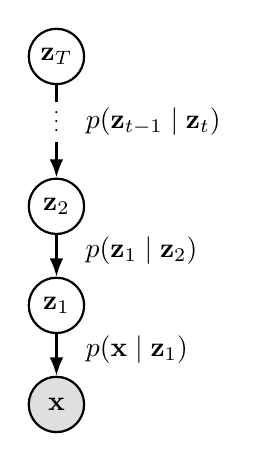
\begin{tikzpicture}[thick,scale=1, every node/.style={scale=1}]
            \node[latent] (zt) {$\mathbf{z}_T$};
            \draw node[draw=none, scale=0.75, below=6pt of zt] (z3) {\hspace{0.5pt}\rotatebox{90}{$\mathbf{\cdots}$}};
            \node[latent, below=13pt of z3] (z2) {$\mathbf{z}_2$};
            \node[latent, below=15pt of z2] (z1) {$\mathbf{z}_1$};
            \node[obs, below=15pt of z1] (x) {$\mathbf{x}$};
            \edge[-]{zt}{z3}
            \edge[-{Latex[scale=1.0]}]{z3}{z2}
            \edge[-{Latex[scale=1.0]}]{z2}{z1}
            \edge[-{Latex[scale=1.0]}]{z1}{x}
            \node[latent, draw=none, right=-2pt of z2, yshift=-16pt] (eq2) {$p(\mathbf{z}_1 \mid \mathbf{z}_2)$};
            \node[latent, draw=none, right=-2pt of z1, yshift=-16pt] (eq1) {$p(\mathbf{x} \mid \mathbf{z}_1)$};
            \node[latent, draw=none, right=-2pt of z3, xshift=6pt, yshift=-0pt] (eq3) {$p(\mathbf{z}_{t-1} \mid \mathbf{z}_t)$};
        \end{tikzpicture}
        \caption{Hierarchical Generative Model}
    \end{subfigure}
    \hfill
    \begin{subfigure}{.32\columnwidth}
        \centering
        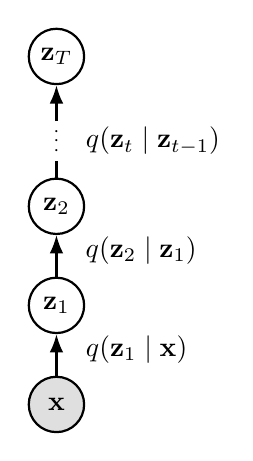
\begin{tikzpicture}[thick,scale=1, every node/.style={scale=1}]
            \node[latent] (zt) {$\mathbf{z}_T$};
            \draw node[draw=none, scale=0.75, below=13pt of zt] (z3) {\hspace{0.5pt}\rotatebox{90}{$\mathbf{\cdots}$}};
            \node[latent, below=6pt of z3] (z2) {$\mathbf{z}_2$};
            \node[latent, below=15pt of z2] (z1) {$\mathbf{z}_1$};
            \node[obs, below=15pt of z1] (x) {$\mathbf{x}$};
            \edge[-{Latex[scale=1.0]}]{z3}{zt}
            \edge[-]{z2}{z3}
            \edge[-{Latex[scale=1.0]}]{z1}{z2}
            \edge[-{Latex[scale=1.0]}]{x}{z1}
            \node[latent, draw=none, right=-2pt of z2, yshift=-16pt] (eq2) {$q(\mathbf{z}_2 \mid \mathbf{z}_1)$};
            \node[latent, draw=none, right=-2pt of z1, yshift=-16pt] (eq1) {$q(\mathbf{z}_1 \mid \mathbf{x})$};
            \node[latent, draw=none, right=-2pt of z3, xshift=6pt, yshift=-0pt] (eq3) {$q(\mathbf{z}_{t} \mid \mathbf{z}_{t-1})$};
        \end{tikzpicture}
        \caption{Bottom-up Inference Model}
    \end{subfigure}
    \hfill
    \begin{subfigure}{.32\columnwidth}
        \centering
        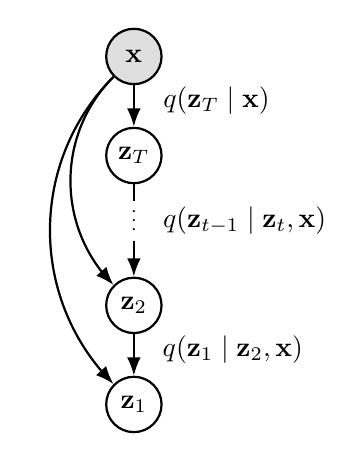
\begin{tikzpicture}[thick,scale=1, every node/.style={scale=1}]
            \node[obs] (x) {$\mathbf{x}$};
            \node[latent, below=15pt of x] (zt) {$\mathbf{z}_T$};
            \draw node[draw=none, scale=0.75, below=6pt of zt] (z3) {\hspace{0.5pt}\rotatebox{90}{$\mathbf{\cdots}$}};
            \node[latent, below=13pt of z3] (z2) {$\mathbf{z}_2$};
            \node[latent, below=15pt of z2] (z1) {$\mathbf{z}_1$};
            \edge[-{Latex[scale=1.0]}]{x}{zt}
            \edge[-]{zt}{z3}
            \edge[-{Latex[scale=1.0]}]{z3}{z2}
            \edge[-{Latex[scale=1.0]}]{z2}{z1}
            \draw [-{Latex[scale=1.0]}] (x) to [out=225,in=135] (z2);
            \draw [-{Latex[scale=1.0]}] (x) to [out=225,in=135] (z1);
            \node[latent, draw=none, right=-2pt of x, yshift=-16pt] (eq1) {$q(\mathbf{z}_T \mid \mathbf{x})$};
            \node[latent, draw=none, right=-2pt of z2, yshift=-16pt] (eq2) {$q(\mathbf{z}_1 \mid \mathbf{z}_2, \mathbf{x})$};
            \node[latent, draw=none, right=-2pt of z3, xshift=6pt, yshift=-0pt] (eq3) {$q(\mathbf{z}_{t-1} \mid \mathbf{z}_{t}, \mathbf{x})$};
        \end{tikzpicture}
        \caption{Top-down Inference Model}
    \end{subfigure}
    \hfill
    \caption{Hierarchical latent variable graphical models. (a) The generative model $p(\mathbf{x}, \mathbf{z}_{1:T})$ of a hierarchical VAE with $T$ latent variables is a Markov chain. (b) The standard \textit{bottom-up} inference model $q(\mathbf{z}_{1:T} \mid \mathbf{x})$ of a hierarchical VAE is a Markov chain in the reverse direction. (c) The \textit{top-down} inference model follows the same topological ordering of the latent variables as the generative model. This top-down structure is used to specify diffusion models. In diffusion models the posterior $q(\mathbf{z}_{1:T} \mid \mathbf{x})$ is tractable due to Gaussian conjugacy, which enables us to specify the \textit{generative} model transitions as $p(\mathbf{z}_{t-1} \mid \mathbf{z}_{t}) = q(\mathbf{z}_{t-1} \mid \mathbf{z}_{t}, \mathbf{x} = \hat{\mathbf{x}}_{\boldsymbol{\theta}}(\mathbf{z}_t; t))$,  where the data $\mathbf{x}$ is replaced by a denoising model $\hat{\mathbf{x}}_{\boldsymbol{\theta}}(\mathbf{z}_t; t)$.
    }
    \label{fig: hvae}
\end{figure}

\subsection{Hierarchical VAE}
\label{subsec: Hierarchical VAE}
A hierarchical VAE is a deep latent variable model comprised of a hierarchy of latent variables $\mathbf{z}_1,\mathbf{z}_2 \dots, \mathbf{z}_T$. Introducing additional (auxiliary) latent variables significantly improves the flexibility of both inference and generative models~\citep{salimans2015markov,ranganath2016hierarchical,maaloe2016auxiliary}.

The joint distribution $p(\mathbf{x}, \mathbf{z}_{1:T})$ specifying a generative model of $\mathbf{x}$ is a variational Markov chain \newline $\mathbf{z}_T \to \mathbf{z}_{T-1} \to \cdots \to \mathbf{z}_1 \to \mathbf{x}$:
%
\begin{align}
    p(\mathbf{x}, \mathbf{z}_{1:T}) &= p(\mathbf{z}_T)p(\mathbf{z}_{T-1} \mid \mathbf{z}_T) \cdots p(\mathbf{z}_1 \mid \mathbf{z}_2) p(\mathbf{x} \mid \mathbf{z}_1)
    \\[5pt] & 
    = p(\mathbf{z}_T) \left[\prod_{t=2}^{T}p(\mathbf{z}_{t-1} \mid \mathbf{z}_t)\right]p(\mathbf{x} \mid \mathbf{z}_1). \label{eq: hvae_gen}
\end{align}
%
The approximate posterior $q(\mathbf{z}_{1:T} \mid \mathbf{x})$ is a Markov chain in the reverse (bottom-up) direction \newline $\mathbf{z}_T \leftarrow \mathbf{z}_{T-1} \leftarrow \cdots \leftarrow \mathbf{z}_1 \leftarrow \mathbf{x}$:
%
\begin{align}
    q(\mathbf{z}_{1:T} \mid \mathbf{x}) &= q(\mathbf{z}_1 \mid \mathbf{x})q(\mathbf{z}_2 \mid \mathbf{z}_1)q(\mathbf{z}_3 \mid \mathbf{z}_2) \cdots q(\mathbf{z}_T \mid \mathbf{z}_{T-1})
    \\[5pt] & 
    = q(\mathbf{z}_1 \mid \mathbf{x}) \prod_{t=2}^{T}q(\mathbf{z}_{t} \mid \mathbf{z}_{t-1}). \label{eq: hvae_inf}
\end{align}
%
The marginal likelihood $p(\mathbf{x})$ is obtained by marginalizing out the latent variables:
%
\begin{align}
    && p(\mathbf{x}) 
    = \int p(\mathbf{x} \mid  \mathbf{z}_{1})p(\mathbf{z}_1) \mathop{\mathrm{d}\mathbf{z}_{1}},
    &&
    % \mathrm{where}&&
    p(\mathbf{z}_t) 
    = \int p(\mathbf{z}_t \mid  \mathbf{z}_{t+1})p(\mathbf{z}_{t+1}) \mathop{\mathrm{d}\mathbf{z}_{t+1}},&&t = 1,2,\dots,T-1,&&
\end{align}
%
and the model is fit by maximizing the VLB of $\log p(\mathbf{x})$:
%
\begin{align}
    \log p(\mathbf{x}) \geq \mathbb{E}_{q(\mathbf{z}_{1:T} \mid \mathbf{x})} \left[ \log \frac{p(\mathbf{x}, \mathbf{z}_{1:T})}{q(\mathbf{z}_{1:T} \mid \mathbf{x})} \right] \eqqcolon \mathrm{VLB}(\mathbf{x}).
\end{align}
%
\subsection{Generative Feedback}
\label{subsec: Generative Feedback}
%
\begin{wrapfigure}[21]{r}{0.4\textwidth}
    \centering
    \vspace{-28pt}
    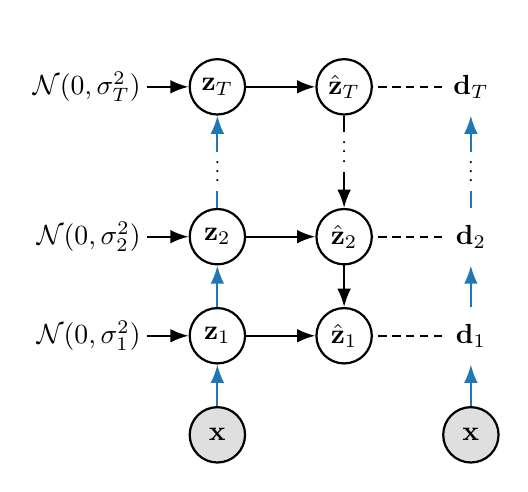
\begin{tikzpicture}[thick,scale=1, every node/.style={scale=1}]
        \node[latent] (zt) {$\hat{\mathbf{z}}_T$};
        \draw node[draw=none, scale=0.75, below=6pt of zt] (z3) {\hspace{0.5pt}\rotatebox{90}{$\mathbf{\cdots}$}};
        \node[latent, below=13pt of z3] (z2) {$\hat{\mathbf{z}}_2$};
        \node[latent, below=15pt of z2] (z1) {$\hat{\mathbf{z}}_1$};
        \edge[-]{zt}{z3}
        \edge[-{Latex[scale=1.0]}]{z3}{z2}
        \edge[-{Latex[scale=1.0]}]{z2}{z1}

        \node[latent, left=25pt of zt] (zzt) {$\mathbf{z}_T$};
        \draw node[draw=none, scale=0.75, below=13pt of zzt] (zz3) {\hspace{0.5pt}\rotatebox{90}{$\mathbf{\cdots}$}};
        \node[latent, left=25pt of z2] (zz2) {$\mathbf{z}_2$};
        \node[latent, left=25pt of z1] (zz1) {$\mathbf{z}_1$};
        \node[obs, below=15pt of zz1] (xx) {$\mathbf{x}$};

        \node[latent, draw=none, left=15pt of zzt] (st) {$\mathcal{N}(0,\sigma_T^2)$};
        \edge[-{Latex[scale=1.0]}]{st}{zzt}
        \node[latent, draw=none, left=15pt of zz2] (s2) {$\mathcal{N}(0,\sigma_2^2)$};
        \edge[-{Latex[scale=1.0]}]{s2}{zz2}
        \node[latent, draw=none, left=15pt of zz1] (s1) {$\mathcal{N}(0,\sigma_1^2)$};
        \edge[-{Latex[scale=1.0]}]{s1}{zz1}

        \node[latent, draw=none, right=25pt of zt] (dt) {$\mathbf{d}_T$};
        \draw node[draw=none, scale=0.75, below=13pt of dt] (d3) {\hspace{0.5pt}\rotatebox{90}{$\mathbf{\cdots}$}};
        \node[latent, draw=none, right=25pt of z2] (d2) {$\mathbf{d}_2$};
        \node[latent, draw=none, right=25pt of z1] (d1) {$\mathbf{d}_1$};
        \node[obs, below=15pt of d1] (x) {$\mathbf{x}$};
        
        \edge[blue, -{Latex[scale=1.0]}]{d3}{dt}
        \edge[blue, -]{d2}{d3}
        \edge[blue, -{Latex[scale=1.0]}]{d1}{d2}
        \edge[blue, -{Latex[scale=1.0]}]{x}{d1}
        \edge[densely dashed,-]{dt}{zt}
        \edge[densely dashed,-]{d2}{z2}
        \edge[densely dashed,-]{d1}{z1}
        \edge[blue,-{Latex[scale=1.0]}]{xx}{zz1}
        \edge[blue,-{Latex[scale=1.0]}]{zz1}{zz2}
        \edge[blue,-]{zz2}{zz3}
        \edge[blue,-{Latex[scale=1.0]}]{zz3}{zzt}
        \edge[-{Latex[scale=1.0]}]{zzt}{zt}
        \edge[-{Latex[scale=1.0]}]{zz2}{z2}
        \edge[-{Latex[scale=1.0]}]{zz1}{z1}
    \end{tikzpicture}
    \caption{A Ladder Network. The latent variables $\mathbf{z}_1, \mathbf{z}_2, \dots, \mathbf{z}_T$ are noisy representations of $\mathbf{x}$, and $\mathbf{d}_1, \mathbf{d}_2, \dots, \mathbf{d}_T$ are clean representations; both sets are produced by a shared encoder (blue arrows). The variables $\hat{\mathbf{z}}_1, \hat{\mathbf{z}}_2, \dots, \hat{\mathbf{z}}_T$ are outputs of denoising functions where $\hat{\mathbf{z}}_t = g_t(\mathbf{z}_t, \hat{\mathbf{z}}_{t+1})$. Notice how $g_t(\cdot)$ receives both bottom-up and top-down information. The dashed horizontal lines denote local cost functions used to minimize  $\|\hat{\mathbf{z}}_t - \mathbf{d}_t \|^2_2$. The main difference compared to denoising diffusion models is that here the denoising targets $\mathbf{d}_t$ are learned representations of $\mathbf{x}$.
    }
    \label{fig: ladder}
\end{wrapfigure}
%
The trouble with hierarchical latent variable models with bottom-up inference is bottom-up inference.~\cite{burda2015importance} and~\cite{sonderby2016ladder} both found hierarchical models with purely bottom-up inference are typically not capable of utilizing more than two layers of latent variables. This often manifests as \textit{posterior collapse}, whereby the posterior distribution (of the top-most layer, say) collapses to a standard Gaussian prior, failing to learn meaningful representations and effectively deactivating latent variables.

To understand why bottom-up inference is challenging for even modestly deep hierarchies, we start by noting the asymmetry between the associated generative and inference models in Equations~\ref{eq: hvae_gen} and~\ref{eq: hvae_inf} respectively.~\cite{burda2015importance,sohl2015deep} point this out as a source of difficulty in training the inference model efficiently, since there is no way to express each term in the VLB as an expectation under a distribution over a single latent variable.~\cite{luo2022understanding} present a similar efficiency-based argument against using bottom-up inference in hierarchical latent variable models.

We claim that efficiency arguments paint an incomplete picture; the main reason one should avoid bottom-up inference is the lack of direct \textit{feedback} from the generative model.
To show why generative feedback is important, we stress that the purpose of the inference model is to perform \textit{Bayesian inference} at any given layer in the hierarchy. That is, to compute the posterior distribution $q(\mathbf{z}_t \mid \mathbf{x})$ over each latent variable $\mathbf{z}_t$:
%
\begin{align}
    & q(\mathbf{z}_t \mid \mathbf{x}) = \frac{p(\mathbf{x} \mid \mathbf{z}_t)p(\mathbf{z}_t)}{p(\mathbf{x})}
    \propto p(\mathbf{x} \mid \mathbf{z}_t) \int p(\mathbf{z}_t \mid  \mathbf{z}_{t+1})p(\mathbf{z}_{t+1}) \mathop{\mathrm{d}\mathbf{z}_{t+1}}, \label{eq: qzx_bayes}
\end{align}
%
which clearly shows that the posterior is not only proportional to the current layer's prior $p(\mathbf{z}_t)$ but also to the layer above's $p(\mathbf{z}_{t+1})$, and so on, following the reverse of the generative Markov chain (Equation~\ref{eq: hvae_gen}). 

It therefore stands to reason that interleaving feedback from each transition in the generative model into each respective transition in the inference model can only make the inference network more accurate. To that end, we can take Equation~\ref{eq: qzx_bayes} and rewrite the posterior distribution over each $\mathbf{z}_t$ such that it contains a more explicit dependency on the preceding latent variables as prescribed:
%
\begin{align}
    & q(\mathbf{z}_t \mid \mathbf{x}) = \int q(\mathbf{z}_t \mid \mathbf{z}_{t+1}, \mathbf{x}) \mathop{\mathrm{d}\mathbf{z}_{t+1}} 
    % \\[5pt] & 
    \propto \int p(\mathbf{x} \mid \mathbf{z}_t) p(\mathbf{z}_t \mid  \mathbf{z}_{t+1})p(\mathbf{z}_{t+1})\mathop{\mathrm{d}\mathbf{z}_{t+1}}
    \\[5pt] \implies \ & q(\mathbf{z}_{t-1} \mid \mathbf{z}_{t}, \mathbf{x}) \propto p(\mathbf{x} \mid \mathbf{z}_{t-1}) p(\mathbf{z}_{t-1} \mid  \mathbf{z}_{t})p(\mathbf{z}_{t}).
\end{align}
%
The posterior $q(\mathbf{z}_{t-1} \mid \mathbf{z}_{t}, \mathbf{x})$ now follows the same topological ordering of the latent variables as the prior $p(\mathbf{z}_{t-1} \mid \mathbf{z}_t)$, and it coincides with the \textit{top-down} inference model in HVAEs~\citep{sonderby2016ladder,kingma2016improved}. Figure~\ref{fig: hvae} shows how this top-down structure compares to the bottom-up approach. An added benefit of the top-down approach is that the generative model can also receive data-dependent feedback from the inference procedure, which~\cite{sonderby2016ladder} found to be beneficial in practice. 

\cite{valpola2015neural,rasmus2015semi} were the first to introduce such lateral feedback connections between the inference and generative paths in hierarchical latent variable models. They called their denoising autoencoder a \textit{ladder network} (see Figure~\ref{fig: ladder}), which later inspired the ladder VAE~\citep{sonderby2016ladder}.~\cite{valpola2015neural} argue that incorporating lateral feedback connections enables the higher layers to learn abstract invariant representations as they no longer have to retain all the details about the input. Concretely, as depicted in Figure~\ref{fig: ladder}, each denoised variable $\hat{\mathbf{z}}_t \coloneqq g_t(\mathbf{z}_t, \hat{\mathbf{z}}_{t+1})$ is computed using a denoising function $g_t(\cdot)$ which receives bottom-up feedback from $\mathbf{z}_t$ and top-down feedback from $\hat{\mathbf{z}}_{t+1}$.
%
\subsection{Top-down Inference}
\label{subsec: Top-down Inference Model}
%
The joint approximate posterior $q(\mathbf{z}_{1:T} \mid \mathbf{x})$ can be alternatively factorized into the \textit{top-down} inference model~\citep{sonderby2016ladder,kingma2016improved}. As mentioned in Section~\ref{subsec: Generative Feedback}, the top-down inference model follows the same topological ordering of the latent variables as the generative model, that is:
%
\begin{align}
    q(\mathbf{z}_{1:T} \mid \mathbf{x}) & = q(\mathbf{z}_T \mid \mathbf{x}) q(\mathbf{z}_{T-1} \mid \mathbf{z}_{T}, \mathbf{x}) \cdots q(\mathbf{z}_2 \mid \mathbf{z}_3, \mathbf{x})q(\mathbf{z}_1 \mid \mathbf{z}_2, \mathbf{x})
    \\[5pt] & 
    = q(\mathbf{z}_T \mid \mathbf{x}) \prod_{t=2}^{T} q(\mathbf{z}_{t-1} \mid \mathbf{z}_t, \mathbf{x}).
\end{align}
%
Variants of the top-down inference model have featured in much deeper state-of-the-art HVAEs for sample generation~\citep{maaloe2019biva,vahdat2020nvae,child2020very,shu2022bit} and approximate counterfactual inference~\citep{pmlr-v202-de-sousa-ribeiro23a,monteiro2022measuring}. As we will explain later, the top-down hierarchical latent variable model serves as the basis for parameterizing denoising diffusion models~\citep{sohl2015deep,ho2020denoising,kingma2021variational}. 

For now, we derive the corresponding VLB to obtain a concrete optimization objective:
%
\begin{align}
    \mathrm{VLB}(\mathbf{x}) & = \mathbb{E}_{q(\mathbf{z}_{1:T} \mid \mathbf{x})} \left[ \log \frac{p(\mathbf{x}, \mathbf{z}_{1:T})}{q(\mathbf{z}_{1:T} \mid \mathbf{x})} \right]
    \\[5pt] & = \mathbb{E}_{q(\mathbf{z}_{1:T} \mid \mathbf{x})} \left[ \log \frac{p(\mathbf{z}_T) p(\mathbf{x} \mid \mathbf{z}_1) \prod_{t=2}^{T}p(\mathbf{z}_{t-1} \mid \mathbf{z}_t)}{q(\mathbf{z}_T \mid \mathbf{x}) \prod_{t=2}^{T} q(\mathbf{z}_{t-1} \mid \mathbf{z}_t, \mathbf{x})} \right] \customtag{factor the joint}
    \\[5pt] & = \mathbb{E}_{q(\mathbf{z}_{1:T} \mid \mathbf{x})}\left[\log p(\mathbf{x} \mid \mathbf{z}_{1}) + \log \frac{p(\mathbf{z}_T)}{ q(\mathbf{z}_T \mid \mathbf{x})}\right] + \mathbb{E}_{q(\mathbf{z}_{1:T} \mid \mathbf{x})}\left[\sum_{t=2}^T \log  \frac{p(\mathbf{z}_{t-1} \mid \mathbf{z}_t)}{q(\mathbf{z}_{t-1} \mid \mathbf{z}_t, \mathbf{x})} \right]
    \\[5pt] & = \mathbb{E}_{q(\mathbf{z}_{1} \mid  \mathbf{x})}\left[\log p(\mathbf{x} \mid \mathbf{z}_{1})\right] + \mathbb{E}_{q(\mathbf{z}_{T} \mid \mathbf{x})}\left[\log \frac{p(\mathbf{z}_T)}{ q(\mathbf{z}_T \mid \mathbf{x})}\right] \nonumber \\[2pt] & \qquad\qquad\qquad\qquad\qquad\qquad\qquad + \sum_{t=2}^T \mathbb{E}_{q(\mathbf{z}_{t-1}, \mathbf{z}_{t} \mid \mathbf{x})} \left[\log \frac{p(\mathbf{z}_{t-1} \mid \mathbf{z}_t)}{q(\mathbf{z}_{t-1} \mid \mathbf{z}_t, \mathbf{x})} \right]
    \\[5pt] & = \mathbb{E}_{q(\mathbf{z}_{1} \mid  \mathbf{x})}\left[\log p(\mathbf{x} \mid \mathbf{z}_{1})\right] + \mathbb{E}_{q(\mathbf{z}_{T} \mid \mathbf{x})}\left[\log \frac{p(\mathbf{z}_T)}{ q(\mathbf{z}_T \mid \mathbf{x})}\right] \nonumber \\[2pt] & \qquad\qquad\qquad\qquad\qquad\qquad\qquad + \sum_{t=2}^T \mathbb{E}_{q(\mathbf{z}_{t} \mid \mathbf{x})} \left[\mathbb{E}_{q(\mathbf{z}_{t-1} \mid \mathbf{z}_{t}, \mathbf{x})} \left[ \log \frac{p(\mathbf{z}_{t-1} \mid \mathbf{z}_t)}{q(\mathbf{z}_{t-1} \mid \mathbf{z}_t, \mathbf{x})} \right]\right]
    \\[5pt] & = \mathbb{E}_{q(\mathbf{z}_{1} \mid \mathbf{x})}\left[\log p(\mathbf{x} \mid \mathbf{z}_{1})\right] - D_{\mathrm{KL}}(q(\mathbf{z}_{T} \mid \mathbf{x}) \parallel p(\mathbf{z}_{T})) \nonumber \\[2pt] & \qquad\qquad\qquad\qquad\qquad\qquad\qquad - \sum_{t=2}^T \mathbb{E}_{q(\mathbf{z}_{t} \mid \mathbf{x})} \left[D_{\mathrm{KL}}(q(\mathbf{z}_{t-1} \mid \mathbf{z}_{t}, \mathbf{x}) \parallel p(\mathbf{z}_{t-1} \mid \mathbf{z}_{t}))\right]. \label{eq: hvae_elbo}
\end{align}
%
It is well worth dedicating some time to understanding the details of the above derivation and the resulting expression, as it is the \textit{exact} objective optimized by diffusion models as well.

One thing to notice is that it comprises the familiar trade-off between minimizing input reconstruction error and keeping the (hierarchical) approximate posterior $q(\mathbf{z}_{1:T} \mid \mathbf{x})$ close to the prior $p(\mathbf{z}_{1:T})$. In contrast to standard VAEs, the prior in HVAEs is learned from data rather than being fixed, as this affords greater flexibility~\citep{kingma2016improved,hoffman2016elbo,tomczak2018vae}.

%
\begin{figure}
    \centering
    \begin{subfigure}{\columnwidth}
    \centering  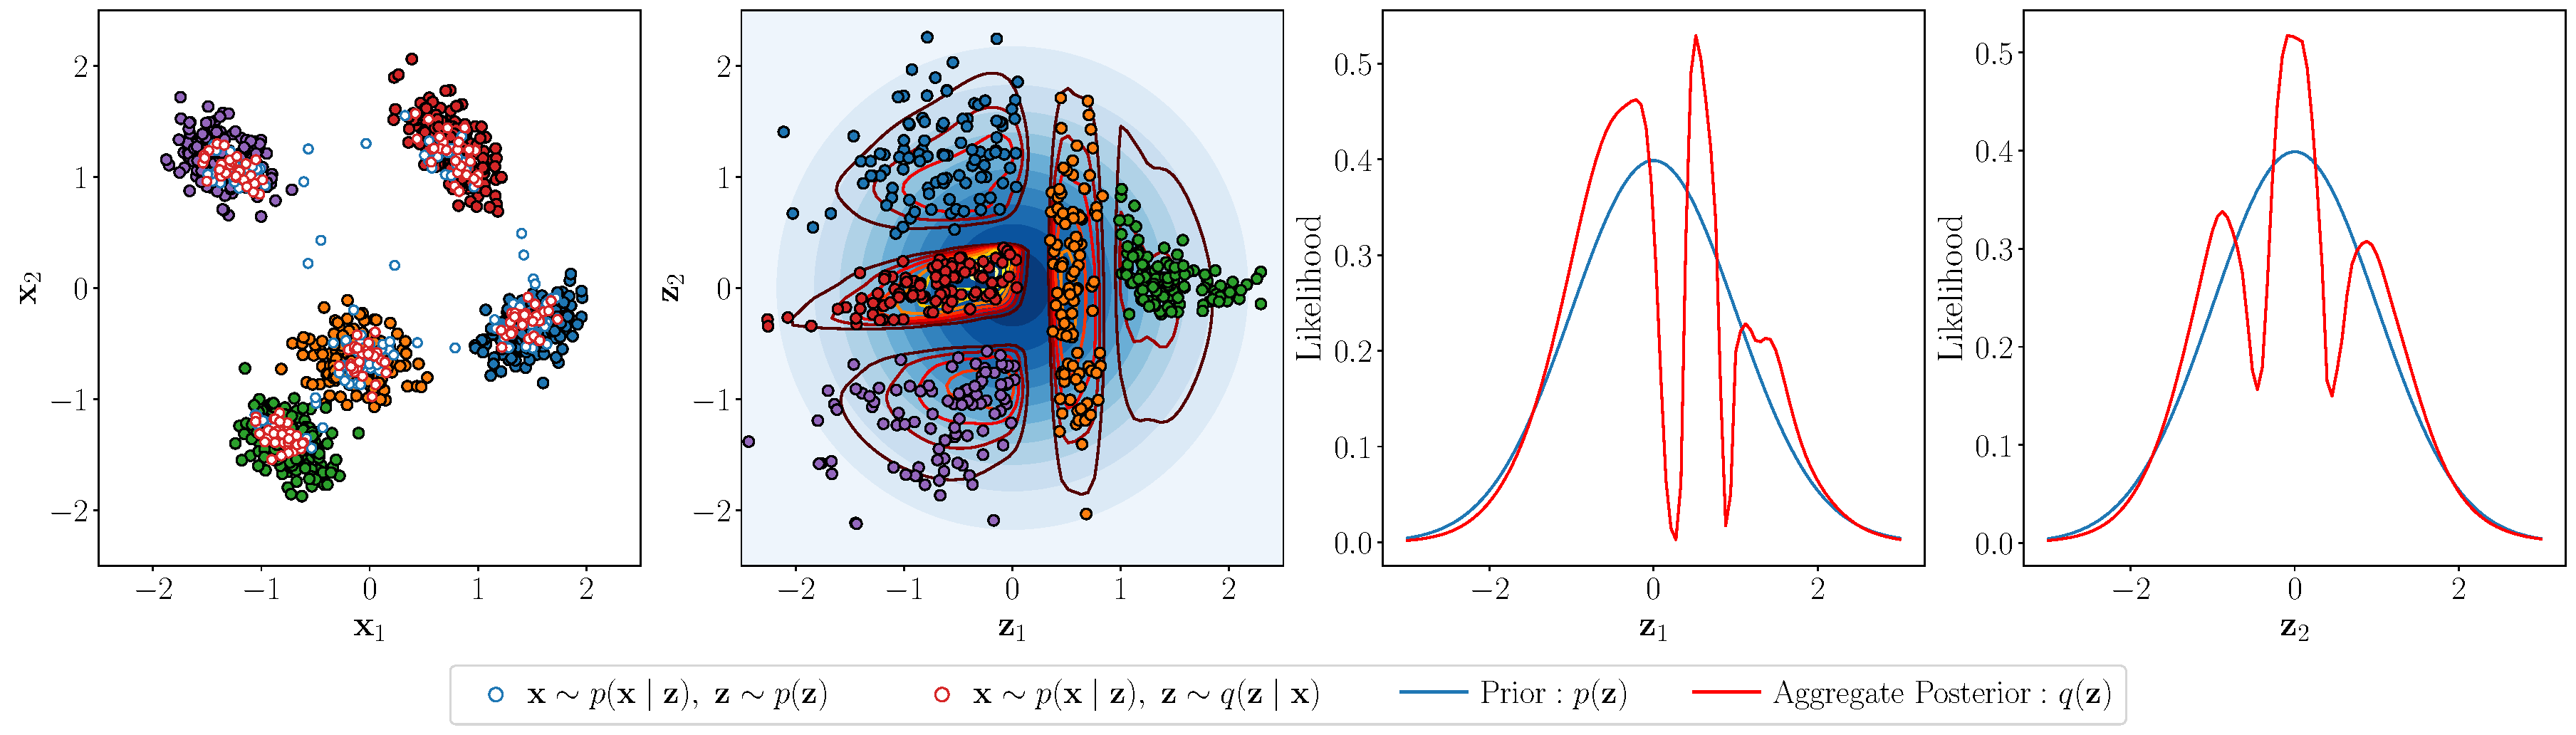
\includegraphics[trim=0 50 0 0, clip, width=\textwidth]{figures/hole2.pdf}
    \end{subfigure}
    \begin{subfigure}{\columnwidth}
    \centering    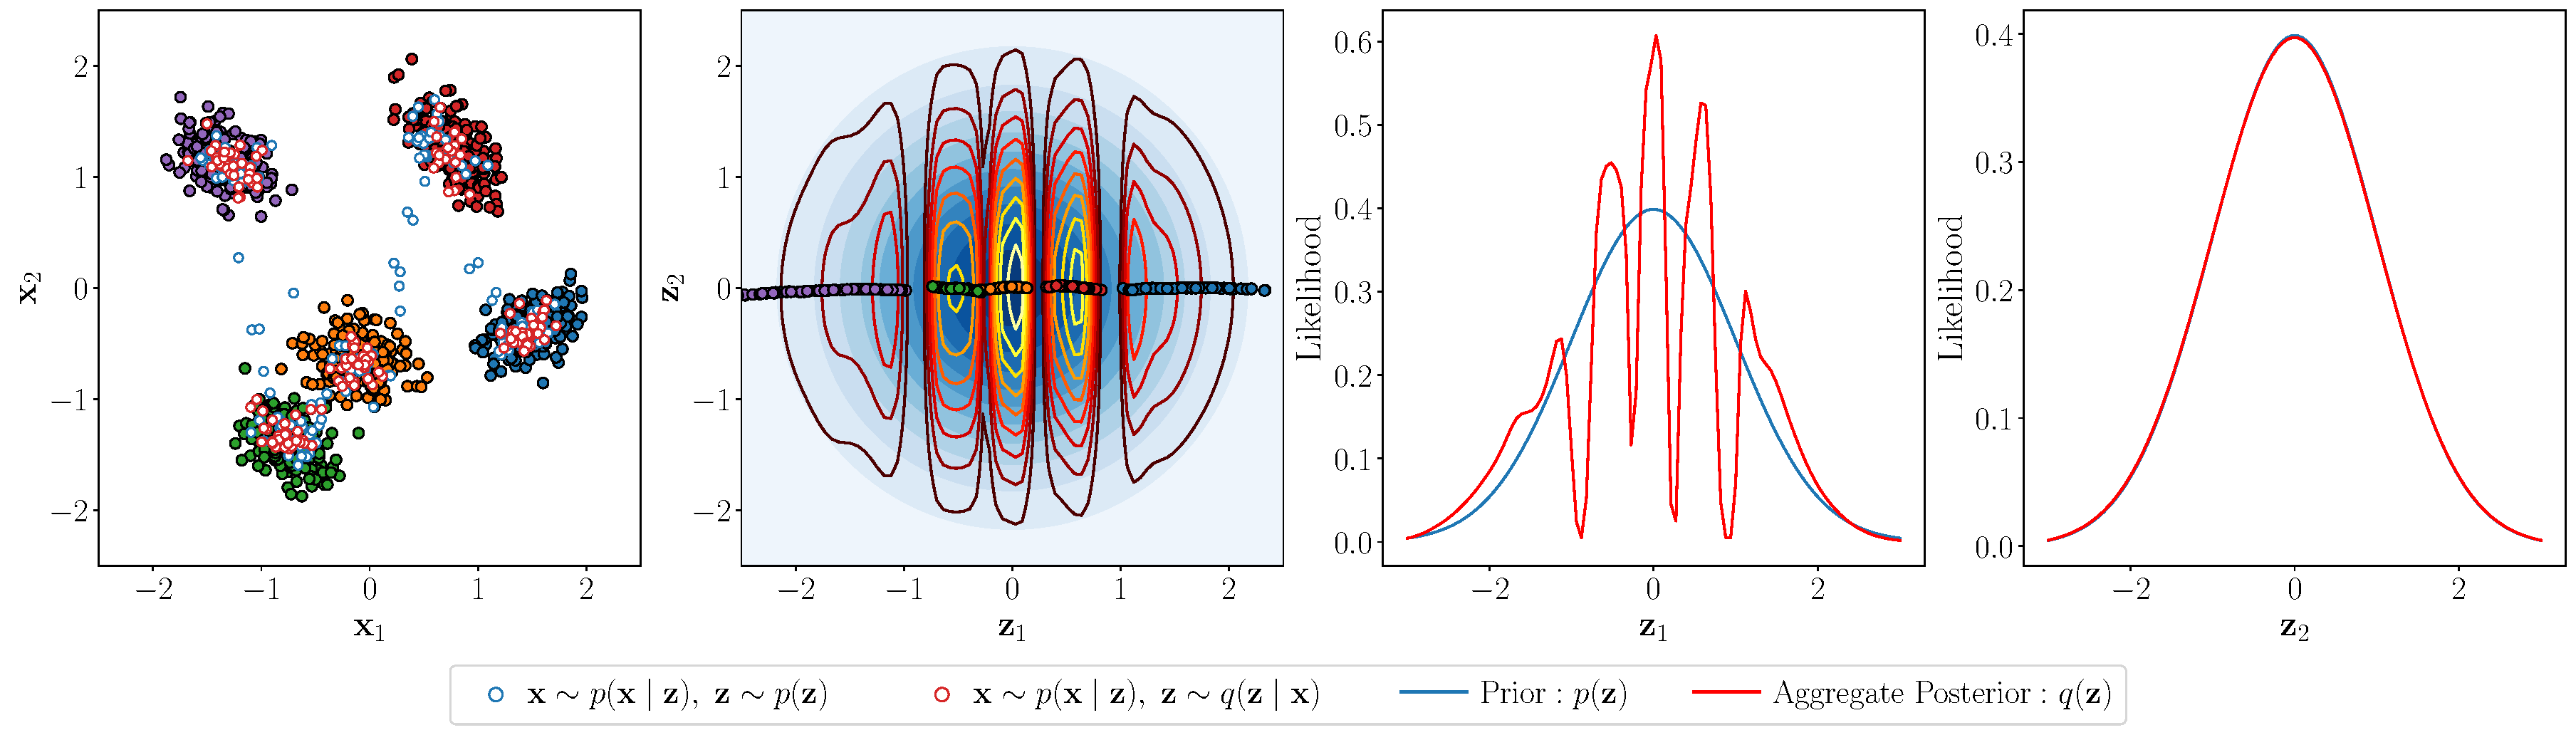
\includegraphics[width=\textwidth]{figures/hole.pdf}
    \end{subfigure}
    \caption{Demonstration of the \textit{hole problem} in VAEs. Results are from a single stochastic layer VAE trained on a 2D toy dataset with five clusters. The latent variable $\mathbf{z}$ is also 2-dimensional for illustration purposes.
    The leftmost column shows the dataset, overlaid with reconstructed datapoints (red border) and random samples from the generative model (blue border). The remaining columns show the assumed prior $p(\mathbf{z}) = \mathcal{N}(\mathbf{z};0, \mathbf{I})$ (blue contours) overlaid with the aggregate posterior $q(\mathbf{z}) = \sum_{i=1}^N q(\mathbf{z} \mid \mathbf{x}_i) / N$. As shown, there are regions with high density under the prior which are assigned low density under the aggregate posterior. This affects the quality of the random samples since we are likely to sample from regions in $p(\mathbf{z})$ not covered by the data. Further, the bottom row shows a common occurrence in VAEs where latent variable(s) are not activated/used at all by the model, in this case, $\mathbf{z}_2$ was not used.
    }
    \label{fig: hole}
\end{figure}
%
\paragraph{The Problem with VAEs.}
%
A primary issue with VAEs is the \textit{hole problem}~\citep{rezende2018taming}. The hole problem refers to the mismatch between the so-called aggregate posterior $q(\mathbf{z})$ and the prior $p(\mathbf{z})$ over the latent variables~\citep{makhzani2015adversarial,hoffman2016elbo}. The aggregate posterior is simply the average posterior distribution over the dataset $\mathcal{D} = \{\mathbf{x}_i\}_{i=1}^N$, that is:
%
\begin{align}
    &&q(\mathbf{z}) = \int q(\mathbf{z} \mid \mathbf{x})p_\mathcal{D}(\mathbf{x}) \mathop{\mathrm{d}\mathbf{x}} 
    , && p_{\mathcal{D}}(\mathbf{x}) = \frac{1}{N}\sum_{i=1}^N \delta(\mathbf{x} - \mathbf{x}_i),&&
\end{align}
%
where $p_\mathcal{D}(\mathbf{x})$ is the \textit{empirical distribution}, constructed by a Dirac delta function $\delta(\cdot)$ centered on each training datapoint $\mathbf{x}_i$. As shown in Figure~\ref{fig: hole}, there can be regions with \textit{high} probability density under the prior which have \textit{low} density under the aggregate posterior. This affects the quality of generated samples when the decoder receives $\mathbf{z}$'s sampled from regions not covered by the data. As we will show, diffusion models circumvent this by defining the aggregate posterior to be equal to the prior by construction.
\newpage
\section{Variational Diffusion Models}
\label{sec: variational diffusion models}
%
\begin{figure}[!t]
    \centering
    \hfill
    \begin{subfigure}{.24\columnwidth}
        \centering
        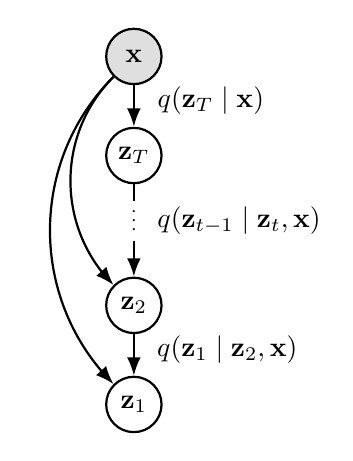
\begin{tikzpicture}[thick,scale=1, every node/.style={scale=1}]
            \node[obs] (x) {$\mathbf{x}$};
            \node[latent, below=15pt of x] (zt) {$\mathbf{z}_T$};
            \draw node[draw=none, scale=0.75, below=6pt of zt] (z3) {\hspace{0.5pt}\rotatebox{90}{$\mathbf{\cdots}$}};
            \node[latent, below=13pt of z3] (z2) {$\mathbf{z}_2$};
            \node[latent, below=15pt of z2] (z1) {$\mathbf{z}_1$};
            \edge[-{Latex[scale=1.0]}]{x}{zt}
            \edge[-]{zt}{z3}
            \edge[-{Latex[scale=1.0]}]{z3}{z2}
            \edge[-{Latex[scale=1.0]}]{z2}{z1}
            \draw [-{Latex[scale=1.0]}] (x) to [out=225,in=135] (z2);
            \draw [-{Latex[scale=1.0]}] (x) to [out=225,in=135] (z1);
            \node[latent, draw=none, right=-4pt of x, yshift=-16pt] (eq1) {$q(\mathbf{z}_T \mid \mathbf{x})$};
            \node[latent, draw=none, right=-4pt of z2, yshift=-16pt] (eq2) {$q(\mathbf{z}_1 \mid \mathbf{z}_2, \mathbf{x})$};
            \node[latent, draw=none, right=-4pt of z3, xshift=6pt, yshift=-0pt] (eq3) {$q(\mathbf{z}_{t-1} \mid \mathbf{z}_{t}, \mathbf{x})$};
        \end{tikzpicture}
        \caption{Top-down Hierarchy}
    \end{subfigure}
    \hfill
    \begin{subfigure}{.2\columnwidth}
        \centering
        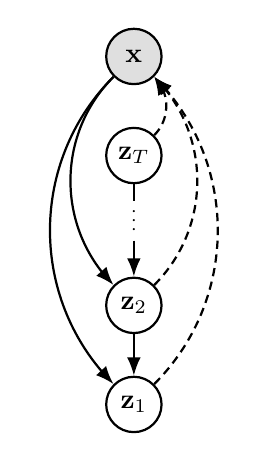
\begin{tikzpicture}[thick,scale=1, every node/.style={scale=1}]
            \node[obs] (x) {$\mathbf{x}$};
            \node[latent, below=15pt of x] (zt) {$\mathbf{z}_T$};
            \draw node[draw=none, scale=0.75, below=6pt of zt] (z3) {\hspace{0.5pt}\rotatebox{90}{$\mathbf{\cdots}$}};
            \node[latent, below=13pt of z3] (z2) {$\mathbf{z}_2$};
            \node[latent, below=15pt of z2] (z1) {$\mathbf{z}_1$};
            \edge[-]{zt}{z3}
            \edge[-{Latex[scale=1.0]}]{z3}{z2}
            \edge[-{Latex[scale=1.0]}]{z2}{z1}
            \draw [-{Latex[scale=1.0]}] (x) to [out=225,in=135] (z2);
            \draw [-{Latex[scale=1.0]}] (x) to [out=225,in=135] (z1);
            \draw [densely dashed, -{Latex[scale=1.0]}] (zt) to [out=45,in=-45] (x);
            \draw [densely dashed, -{Latex[scale=1.0]}] (z2) to [out=45,in=-45] (x);
            \draw [densely dashed, -{Latex[scale=1.0]}] (z1) to [out=45,in=-45] (x);
        \end{tikzpicture}
        \caption{Diffusion Model}
    \end{subfigure}
    \hfill
    \begin{subfigure}{.26\columnwidth}
        \centering       
        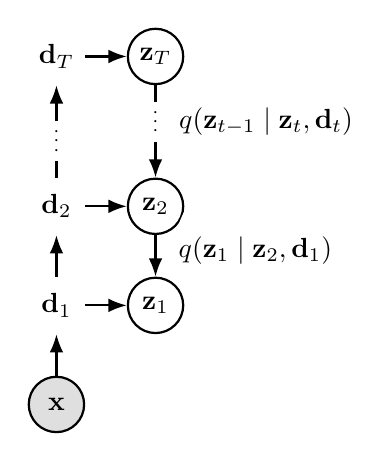
\begin{tikzpicture}[thick,scale=1, every node/.style={scale=1}]
            \node[latent] (zt) {$\mathbf{z}_T$};
            \draw node[draw=none, scale=0.75, below=6pt of zt] (z3) {\hspace{0.5pt}\rotatebox{90}{$\mathbf{\cdots}$}};
            \node[latent, below=13pt of z3] (z2) {$\mathbf{z}_2$};
            \node[latent, below=15pt of z2] (z1) {$\mathbf{z}_1$};
            \edge[-]{zt}{z3}
            \edge[-{Latex[scale=1.0]}]{z3}{z2}
            \edge[-{Latex[scale=1.0]}]{z2}{z1}
            \node[latent, draw=none, right=-4pt of z2, yshift=-16pt] (eq2) {$q(\mathbf{z}_1 \mid \mathbf{z}_2, \mathbf{d}_1)$};
            \node[latent, draw=none, right=-4pt of z3, xshift=6pt, yshift=-0pt] (eq3) {$q(\mathbf{z}_{t-1} \mid \mathbf{z}_t, \mathbf{d}_t)$};

            \node[latent, draw=none, left=15pt of zt] (dt) {$\mathbf{d}_T$};
            \draw node[draw=none, scale=0.75, below=13pt of dt] (d3) {\hspace{0.5pt}\rotatebox{90}{$\mathbf{\cdots}$}};
            \node[latent, draw=none, left=15pt of z2] (d2) {$\mathbf{d}_2$};
            \node[latent, draw=none, left=15pt of z1] (d1) {$\mathbf{d}_1$};
            \node[obs, below=15pt of d1] (x) {$\mathbf{x}$};
            
            \edge[-{Latex[scale=1.0]}]{d3}{dt}
            \edge[-]{d2}{d3}
            \edge[-{Latex[scale=1.0]}]{d1}{d2}
            \edge[-{Latex[scale=1.0]}]{x}{d1}
            \edge[-{Latex[scale=1.0]}]{dt}{zt}
            \edge[-{Latex[scale=1.0]}]{d2}{z2}
            \edge[-{Latex[scale=1.0]}]{d1}{z1}
        \end{tikzpicture}
        \caption{HVAE Inference Model}
    \end{subfigure}
    \hfill
    \begin{subfigure}{.26\columnwidth}
        \centering
        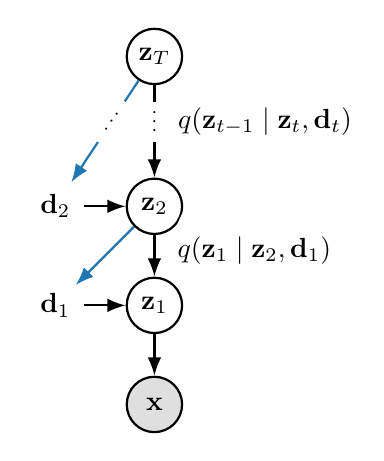
\begin{tikzpicture}[thick,scale=1, every node/.style={scale=1}]
            \node[latent, below] (zt) {$\mathbf{z}_T$};
            \draw node[draw=none, scale=0.75, below=6pt of zt] (z3) {\hspace{0.5pt}\rotatebox{90}{$\mathbf{\cdots}$}};
            \node[latent, below=13pt of z3] (z2) {$\mathbf{z}_2$};
            \node[latent, below=15pt of z2] (z1) {$\mathbf{z}_1$};
            \node[obs, below=15pt of z1] (x) {$\mathbf{x}$};
            \node[latent, draw=none, left=15pt of z1] (d1) {${\mathbf{d}}_1$};
            \node[latent, draw=none, left=15pt of z2] (d2) {${\mathbf{d}}_2$};

            \draw node[draw=none, scale=0.75, left=4pt of z3] (d3) {\hspace{0.5pt}\rotatebox{55}{$\mathbf{\cdots}$}};
            
            \edge[-]{zt}{z3}
            \edge[blue,-]{zt}{d3}
            \edge[blue,-{Latex[scale=1.0]}]{d3}{d2}
            \edge[blue, -{Latex[scale=1.0]}]{z2}{d1}
        
            \edge[-{Latex[scale=1.0]}]{z3}{z2}
            \edge[-{Latex[scale=1.0]}]{z2}{z1}
            \edge[-{Latex[scale=1.0]}]{z1}{x}
            \edge[-{Latex[scale=1.0]}]{d1}{z1}
            \edge[-{Latex[scale=1.0]}]{d2}{z2}

            \node[latent, draw=none, right=-4pt of z2, yshift=-16pt] (eq2) {$q(\mathbf{z}_1 \mid \mathbf{z}_2, \mathbf{d}_1)$};
            \node[latent, draw=none, right=-4pt of z3, xshift=6pt, yshift=-0pt] (eq3) {$q(\mathbf{z}_{t-1} \mid \mathbf{z}_{t}, \mathbf{d}_t)$};
        \end{tikzpicture}
        \caption{Reverse Process}
    \end{subfigure}
    \hfill
    \caption{Probabilistic graphical models of HVAEs and diffusion models. \textbf{(a)} The general top-down hierarchical latent variable model. \textbf{(b)} The top-down model used to specify diffusion models, where $q(\mathbf{z}_T \mid \mathbf{x}) = q(\mathbf{z}_T)$ by construction. Here the posterior $q(\mathbf{z}_{1:T} \mid \mathbf{x})$ is a fixed noising process, so the modelling task is bottom-up prediction of $\mathbf{x}$ from each $\mathbf{z}_t$, i.e. denoising (dashed lines). \textbf{(c)} The top-down model used for posterior inference in HVAEs. It consists of a deterministic bottom-up pass to compute $\mathbf{d}_1,\dots,\mathbf{d}_T$, followed a stochastic top-down pass to compute $\mathbf{z}_T,\dots,\mathbf{z}_1$. \textbf{(d)} The reverse process of a diffusion model, i.e. the generative model. The main differences compared to (c) are that here the deterministic variables $\mathbf{d}_{T-1},\dots,\mathbf{d}_1$ do not depend on $\mathbf{x}$ nor have their own hierarchical dependencies. Further, the {\color{blue}blue} lines represent a denoising model $\hat{\mathbf{x}}_{\boldsymbol{\theta}} :\mathbf{z}_t \to \mathbf{d}_t$ which is \textit{shared} across the hierarchy.
    }
    \label{fig: hvae2}
\end{figure}
%
A diffusion probabilistic model~\citep{sohl2015deep} can be understood as a hierarchical VAE with a particular choice of inference and generative model. Like HVAEs, diffusion models are deep latent variable models that maximize the variational lower bound of the log-likelihood of the data (i.e. the ELBO). Diffusion models were largely inspired by ideas from statistical physics rather than variational Bayesian methods, so they come with a different set of modelling choices and advantages. The general idea behind diffusion models is to define a \textit{fixed} forward (inference) diffusion process that converts any complex data distribution into a tractable distribution, and then learn a generative model that reverses this diffusion process. Figure~\ref{fig: hvae2} compares diffusion models with (top-down inference) HVAEs.

Diffusion probabilistic models have the following distinctive properties:
\begin{enumerate}[(i)]
    \item The joint posterior $q(\mathbf{z}_{1:T} \mid \mathbf{x})$ is fixed rather than learned from observed data. This amounts to having a fixed encoder defining a \textit{Gaussian diffusion process} of the data;
    \item Each latent variable $\mathbf{z}_t$ has the same dimensionality as the input data $\mathbf{x}$;
    \item The aggregate posterior $q(\mathbf{z}_T)$ is equal to the prior $p(\mathbf{z}_T)$ by construction;
    \item The functional form of the inference model is identical to that of the generative model. This corresponds exactly to the top-down inference model structure used in HVAEs;
    \item A single neural network is shared across all levels of the latent variable hierarchy, and each layer can be trained without having to compute the preceding ones;
    \item They maximize a particular \textit{weighted} objective which seems to better align with human perception by suppressing modelling effort on imperceptible details.
\end{enumerate}
%
\begin{figure}[!t]
    \hfill
    \begin{subfigure}{.32\columnwidth}
        \centering
        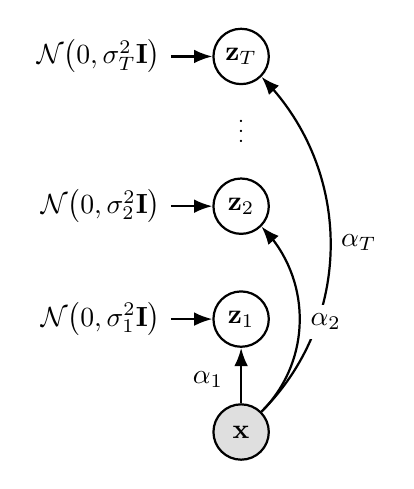
\begin{tikzpicture}[thick,scale=1, every node/.style={scale=1}]
            \node[obs] (x) {$\mathbf{x}$};
            \node[latent, above=20pt of x] (z1) {$\mathbf{z}_1$};
            \node[latent, above=20pt of z1] (z2) {$\mathbf{z}_{2}$};
            \draw node[draw=none, scale=0.8, above=9pt of z2] (z3) {\hspace{0.5pt}\rotatebox{90}{$\mathbf{\cdots}$}};
            \draw [-{Latex[scale=1.0]}] (x) to [out=45,in=-45] (z2);
            \node[latent, above=9pt of z3] (zt) {$\mathbf{z}_T$};
            \edge[-{Latex[scale=1.0]}]{x}{z1}
            \node[rectangle, draw=none, fill=white, scale=1, above=2pt of x, xshift=-12pt] (eq1) {$\alpha_1$};
            \draw [-{Latex[scale=1.0]}] (x) to [out=45,in=-45] (zt);
            \node[rectangle, draw=none, fill=white, scale=1, right=22pt of z2, yshift=-13pt] (eq2) {$\alpha_T$};
            \node[rectangle, draw=none, scale=1, left=15pt of zt] (nt) {$\mathcal{N}\big(0, \sigma^2_T\mathbf{I}\big)$};
            \node[rectangle, draw=none, scale=1, left=15pt of z2] (n2) {$\mathcal{N}\big(0, \sigma^2_2\mathbf{I}\big)$};
            \node[rectangle, draw=none, scale=1, left=15pt of z1] (n1) {$\mathcal{N}\big(0, \sigma^2_1\mathbf{I}\big)$};
            \edge[-{Latex[scale=1.0]}]{nt}{zt}
            \edge[-{Latex[scale=1.0]}]{n2}{z2}
            \edge[-{Latex[scale=1.0]}]{n1}{z1}
            \node[rectangle, draw=none, fill=white, scale=1, right=11pt of z1, yshift=-1pt] (eq2) {$\alpha_2$};
        \end{tikzpicture}
        \caption{Gaussian Diffusion}
        \label{fig: gd}
    \end{subfigure}
    \hfill
    \begin{subfigure}{.32\columnwidth}
        \centering
        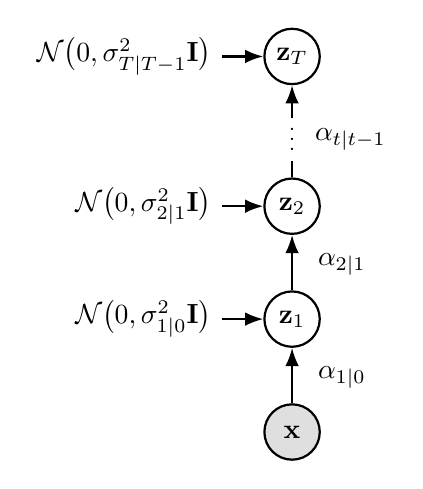
\begin{tikzpicture}[thick,scale=1, every node/.style={scale=1}]
            \node[obs] (x) {$\mathbf{x}$};
            \node[latent, above=20pt of x] (z1) {$\mathbf{z}_1$};
            \node[latent, above=20pt of z1] (z2) {$\mathbf{z}_{2}$};
            \draw node[draw=none, scale=0.8, above=6pt of z2] (z3) {\hspace{0.5pt}\rotatebox{90}{$\mathbf{\cdots}$}};
            \node[latent, above=12pt of z3] (zt) {$\mathbf{z}_T$};
            \edge[-{Latex[scale=1.0]}]{x}{z1}
            \node[rectangle, draw=none, fill=white, scale=1, above=1.5pt of x, xshift=18pt] (eq1) {$\alpha_{1|0}$};
            \node[rectangle, draw=none, fill=white, scale=1, above=1.5pt of z1, xshift=18pt] (eq2) {$\alpha_{2|1}$};
            \node[rectangle, draw=none, fill=white, scale=1, right=-0.4pt of z3] (eq3) {$\alpha_{t|t-1}$};
            
            \edge[-{Latex[scale=1.0]}]{z1}{z2}
            \node[rectangle, draw=none, scale=1, left=15pt of zt] (nt) {$\mathcal{N}\big(0, \sigma^2_{T|T-1}\mathbf{I}\big)$};
            \node[rectangle, draw=none, scale=1, left=15pt of z2] (n2) {$\mathcal{N}\big(0, \sigma^2_{2|1}\mathbf{I}\big)$};
            \node[rectangle, draw=none, scale=1, left=15pt of z1] (n1) {$\mathcal{N}\big(0, \sigma^2_{1|0}\mathbf{I}\big)$};
            \edge[-{Latex[scale=1.0]}]{nt}{zt}
            \edge[-{Latex[scale=1.0]}]{n2}{z2}
            \edge[-{Latex[scale=1.0]}]{n1}{z1}

            \edge[-]{z2}{z3}
            \edge[-{Latex[scale=1.0]}]{z3}{zt}
        \end{tikzpicture}
        \caption{Markovian Transitions}
        \label{fig: mt}
    \end{subfigure}
    \hfill
    \begin{subfigure}{.34\columnwidth}
        \centering
        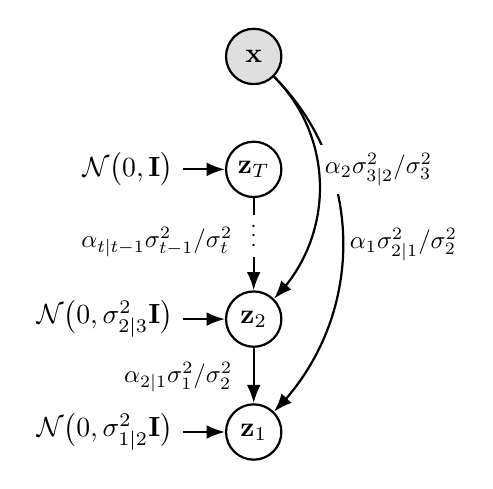
\begin{tikzpicture}[thick,scale=1, every node/.style={scale=1}]
            \node[obs] (x) {$\mathbf{x}$};
            \node[latent, below=20pt of x] (zt) {$\mathbf{z}_T$};
            \draw node[draw=none, scale=0.8, below=6pt of zt] (z3) {\hspace{0.5pt}\rotatebox{90}{$\mathbf{\cdots}$}};
            \node[latent, below=12pt of z3] (z2) {$\mathbf{z}_2$};
            \node[latent, below=20pt of z2] (z1) {$\mathbf{z}_1$};
            \edge[-]{zt}{z3}
            \edge[-{Latex[scale=1.0]}]{z3}{z2}
            \edge[-{Latex[scale=1.0]}]{z2}{z1}
            \node[rectangle, draw=none, fill=white, scale=0.9, right=21pt of z2, yshift=30pt] (eq5) {$\alpha_{1}\sigma^2_{2|1}/\sigma^{2}_{2}$};
            \draw [-{Latex[scale=1.0]}] (x) to [out=-45,in=45] (z1);
            \node[rectangle, draw=none, fill=white, scale=0.9, right=12pt of zt] (eq6) {$\alpha_{2}\sigma^2_{3|2}/\sigma^{2}_{3}$};
            \draw [-{Latex[scale=1.0]}] (x) to [out=-45,in=45] (z2);
            \node[rectangle, draw=none, scale=1, left=15pt of zt] (nt) {$\mathcal{N}\big(0, \mathbf{I}\big)$};
            \node[rectangle, draw=none, scale=1, left=15pt of z2] (n2) {$\mathcal{N}\big(0, \sigma^2_{2|3}\mathbf{I}\big)$};
            \node[rectangle, draw=none, scale=1, left=15pt of z1] (n1) {$\mathcal{N}\big(0, \sigma^2_{1|2}\mathbf{I}\big)$};
            \edge[-{Latex[scale=1.0]}]{nt}{zt}
            \edge[-{Latex[scale=1.0]}]{n2}{z2}
            \edge[-{Latex[scale=1.0]}]{n1}{z1}
            \node[rectangle, draw=none, fill=white, scale=0.9, left=-6pt of z1, yshift=22pt] (eq3) {$\alpha_{2|1}\sigma^2_{1}/\sigma^{2}_{2}$};
            \node[rectangle, draw=none, fill=white, scale=0.9, left=-6pt of z2, yshift=31pt] (eq4) {$\alpha_{t|t-1}\sigma^2_{t-1}/\sigma^{2}_{t}$};
        \end{tikzpicture}
        \caption{Top-down Posterior}
        \label{fig: tdp}
    \end{subfigure}
    \caption{Graphical model(s) describing a discrete-time Gaussian diffusion process ($T$ timesteps in total). \textbf{(a)} Parameterization of the forward process in terms of the conditionals $q(\mathbf{z}_t \mid \mathbf{x})$ (ref. Section~\ref{subsec: Gaussian Diffusion Process: Forward Time}). Each latent variable $\mathbf{z}_t$ is a noisy version of $\mathbf{x}$ given by: $\mathbf{z}_t = \alpha_t \mathbf{x} + \sigma_t \boldsymbol{\epsilon}_t$, and $\boldsymbol{\epsilon}_t \sim \mathcal{N}(0, \mathbf{I})$. \textbf{(b)} Markov chain formed by a sequence of transition distributions $q(\mathbf{z}_t \mid \mathbf{z}_{t-1})$ (ref. Section~\ref{subsubsec: lgt}). Each latent variable is given by: $\mathbf{z}_t = \alpha_{t|t-1} \mathbf{z}_{t-1} + \sigma_{t|t-1} \boldsymbol{\epsilon}_t$, with parameters $\alpha_{t|t-1} \coloneqq \alpha_{t} / \alpha_{t-1}$ and $\sigma^2_{t|t-1} \coloneqq \sigma^2_{t} - \alpha^2_{t|t-1}\sigma^2_{t-1}$. \textbf{(c)} The top-down posterior is tractable due to Gaussian conjugacy: $q(\mathbf{z}_{t-1} \mid \mathbf{z}_t, \mathbf{x}) \propto q(\mathbf{z}_{t} \mid \mathbf{z}_{t-1})q(\mathbf{z}_{t-1} \mid \mathbf{x})$ (ref. Section~\ref{subsubsec: qzs}), where $q(\mathbf{z}_{t-1} \mid \mathbf{x})$ acts as a Gaussian prior and $q(\mathbf{z}_{t} \mid \mathbf{z}_{t-1})$ as a Gaussian likelihood.  
    This top-down posterior is used to specify the \textit{generative} model transitions as $p(\mathbf{z}_{t-1} \mid \mathbf{z}_{t}) = q(\mathbf{z}_{t-1} \mid \mathbf{z}_{t}, \mathbf{x} = \hat{\mathbf{x}}_{\boldsymbol{\theta}}(\mathbf{z}_t; t))$, where the data $\mathbf{x}$ is replaced by a learnable denoising model $\hat{\mathbf{x}}_{\boldsymbol{\theta}}(\mathbf{z}_t; t)$. 
    }
    \label{fig: diffusion_process}
    \hfill
\end{figure}

\newpage
Recent model innovations~\citep{ho2020denoising} -- along with insights from stochastic processes~\citep{anderson1982reverse} and score-based generative modelling~\citep{hyvarinen2005estimation,vincent2011connection,song2019generative,song2021scorebased} -- have yielded a myriad of impressive synthesis results at scale~\citep{nichol2021improved,dhariwal2021diffusion,nichol2022glide,ho2022cascaded,rombach2022high,saharia2022photorealistic,hoogeboom2022equivariant}. 
%

\cite{kingma2021variational,kingma2023understanding} introduced a family of diffusion-based generative models they call Variational Diffusion Models (VDMs), and showed us that: 
%
\begin{enumerate}[(i)]
    \item The latent hierarchy can be made infinitely deep\footnote{This notion was concurrently explored by~\cite{song2021scorebased,huang2021variational,vahdat2021score}.} via a continuous-time model where $T \to \infty$; 
    \item The continuous-time VLB is invariant to the noise schedule\footnote{Except for the signal-to-noise ratio at its endpoints (see Section~\ref{subsubsec: Invariance to the Noise Schedule}).}, meaning we can learn/adapt our noise schedule such that it minimizes the variance of the resulting Monte Carlo estimator of the loss;
    \item Although \textit{weighted} diffusion objectives \textit{appear} markedly different from regular maximum likelihood training, they all implicitly optimize some instance of the ELBO;
    \item VDMs are capable of state-of-the-art image synthesis, showing that standard maximum likelihood-based training objectives (i.e. the ELBO) are not inherently at odds with perceptual quality.
\end{enumerate}

One important distinction to make between HVAEs and diffusion probabilistic models at this stage is that the role of the latent variables $\mathbf{z}_{1:T}$ are very different from a \textit{representation learning} perspective. In HVAEs, the posterior latents $\mathbf{z}_{1:T}$ are useful learned representations of $\mathbf{x}$, which \textit{increase} in semantic informativeness w.r.t. $\mathbf{x}$ as we go from $\mathbf{z}_1$ to $\mathbf{z}_T$. In diffusion probabilistic models, the latent variables $\mathbf{z}_{1:T}$ generally have no semantic meaning, and they \textit{decrease} in informativeness w.r.t. $\mathbf{x}$ as we go from $\mathbf{z}_1$ to $\mathbf{z}_T$. This is because each $\mathbf{z}_t$ is simply a noisy version of $\mathbf{x}$ following a Gaussian diffusion process.
%
\newpage
%
\begin{figure}[!t]
    \begin{subfigure}{\textwidth}
        \centering 
        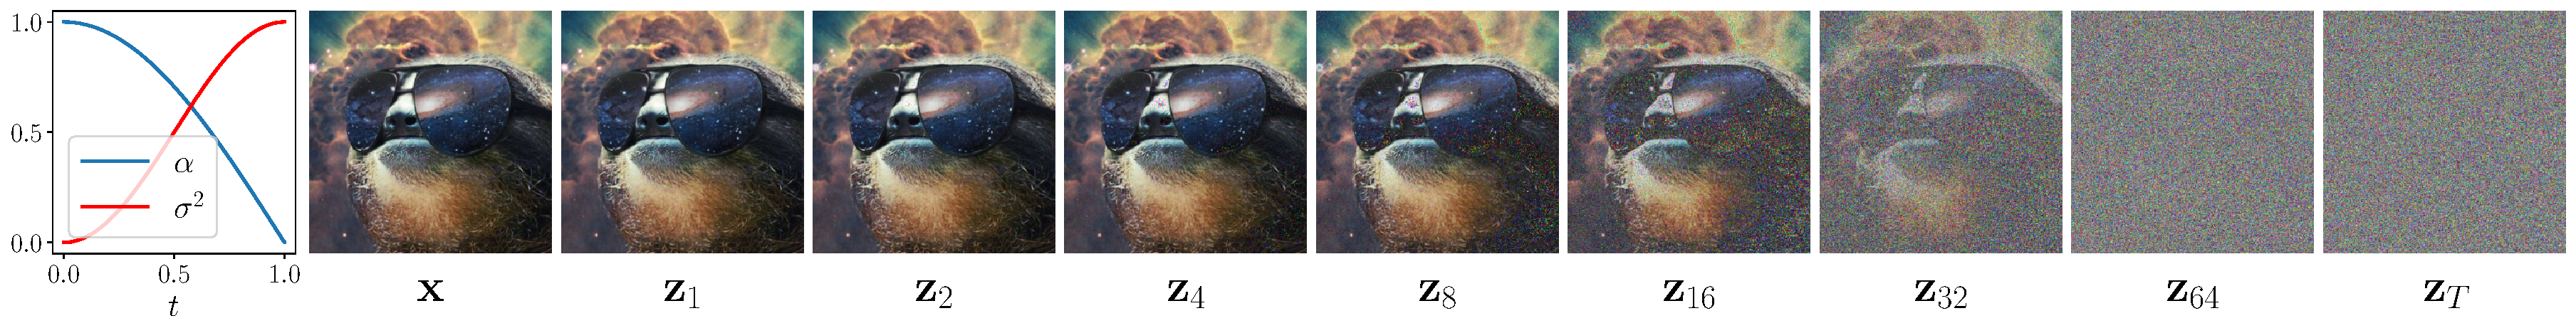
\includegraphics[trim=0 0 0 0,clip,width=\textwidth]{figures/cosine_sloth.pdf}
        \label{fig:cosine_sloth}
    \end{subfigure}
    \\[-8pt]
    \begin{subfigure}{\textwidth}
        \centering 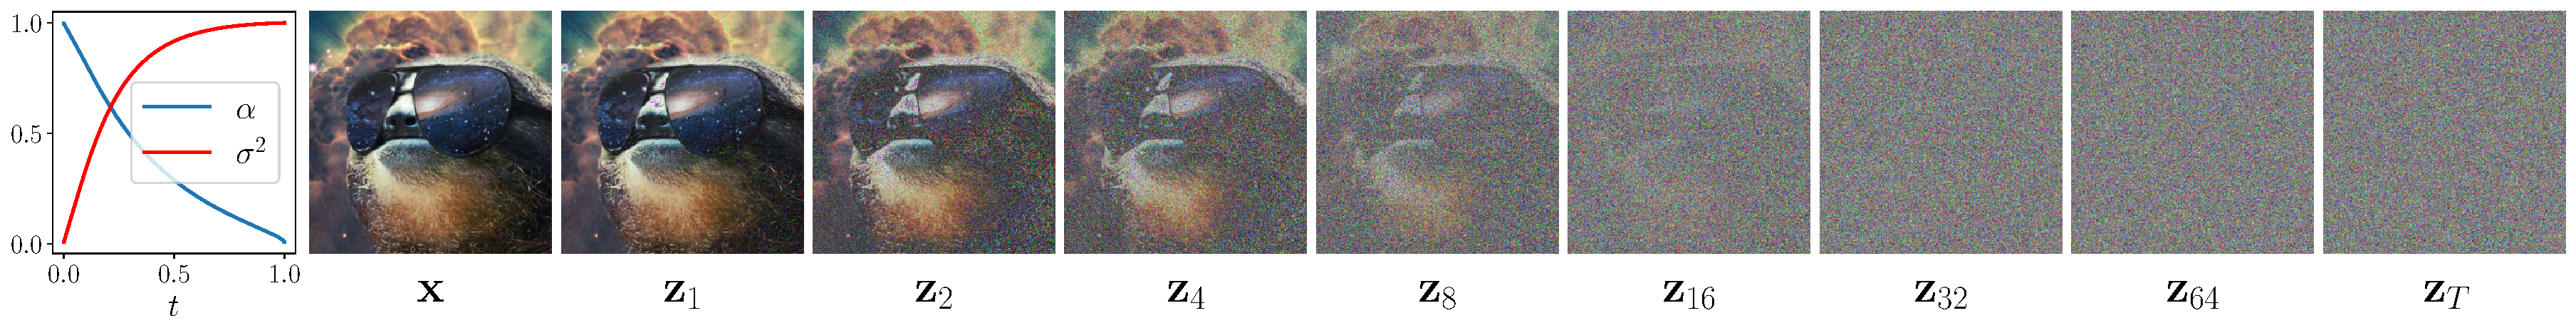
\includegraphics[trim=0 0 0 0,clip,width=\textwidth]{figures/edm_sloth.pdf}
        \label{fig:edm_sloth}
    \end{subfigure}
    \vspace{-20pt}
    \caption{Gaussian diffusion process ($T{=}100$). Showing two popular noise schedules in terms of $\alpha$, $\sigma^2$ as per Section~\ref{subsec: Gaussian Diffusion Process: Forward Time}: (top) cosine~\citep{nichol2021improved}; (bottom) EDM~\citep{karras2022elucidating}.}
    \label{fig: diff_sloth}
\end{figure}
%
\subsection{Forward Process: Gaussian Diffusion}
\label{subsec: Gaussian Diffusion Process: Forward Time}
%
A \textit{Gaussian diffusion process} gradually transforms data $\mathbf{x}$ into random noise by adding increasing amounts of Gaussian noise at each timestep $t=0,\dots,1$ resulting in a set of latent variables $\mathbf{z}_0,\dots,\mathbf{z}_1$.\footnote{For consistency with the continuous-time case where $T \to \infty$, we denote the latent variables as $\mathbf{z}_{0:1}$ rather than $\mathbf{z}_{1:T}$.}
Each latent variable $\mathbf{z}_t$ is simply a noisy version of $\mathbf{x}$, and its distribution conditional on $\mathbf{x}$ is given by:
%
\begin{align}
    && q(\mathbf{z}_t \mid \mathbf{x}) = \mathcal{N}\left(\mathbf{z}_t;\alpha_{t} \mathbf{x}, \sigma^2_{t} \mathbf{I}\right), && \mathbf{z}_t = \alpha_{t} \mathbf{x} + \sigma_{t}\boldsymbol{\epsilon}_t, && \boldsymbol{\epsilon}_t \sim \mathcal{N}\left(\boldsymbol{\epsilon}_t; 0, \mathbf{I}\right),&&
\end{align}
%
where $\alpha_{t} \in (0,1)$ and $\sigma^2_{t} \in (0,1)$ are chosen scalar valued functions of time $t \in [0,1]$. See Figures~\ref{fig: gd},~\ref{fig: diff_sloth}.

The key idea is to define the forward diffusion process such that the noisiest latent variable $\mathbf{z}_1$ at time $t=1$ is standard Gaussian distributed: $q(\mathbf{z}_1 \mid \mathbf{x}) = \mathcal{N}(\mathbf{z}_1; 0, \mathbf{I})$, thus $q(\mathbf{z}_1 \mid \mathbf{x}) = q(\mathbf{z}_1)$. To that end, the scaling coefficients $\alpha_{0} > \ldots > \alpha_{1}$ \textit{decrease} w.r.t. time $t$, whereas the noise variances $\sigma_{0}^2 < \ldots < \sigma_{1}^2$ \textit{increase} w.r.t. $t$. As we will show, this enables us to learn a generative Markov chain which starts from $\mathbf{z}_1 \sim q(\mathbf{z}_1)$ and reverses the forward diffusion process to obtain samples from the data distribution. The implications of this are profound; the \textit{aggregate} posterior $q(\mathbf{z}_1)$ is equal to the prior $p(\mathbf{z}_1)$ by construction, which circumvents the \textit{hole problem} in VAEs (see Figure~\ref{fig: hole}).~\cite{hoffman2016elbo} showed that the optimal prior is the aggregate posterior, as long as our posterior approximation is good enough.

A \textit{variance-preserving} process is achieved by solving for the value of $\alpha_t$ such that the variance of the respective latent variable $\mathbb{V}[\mathbf{z}_t]$ is equal to the variance of the input data $\mathbb{V}[\mathbf{x}]$. This can be important from a modelling perspective, as adding increasing amounts of noise to the input alters its statistics.

We can first apply some basic properties of \textit{variance} to simplify $\mathbb{V}[\mathbf{z}_t]$ as follows:
%
\begin{align}
    \mathbb{V}[\mathbf{z}_t] = \mathbb{V}[\alpha_{t} \mathbf{x} + \sigma_{t}\boldsymbol{\epsilon}_t] = \mathbb{V}[\alpha_{t} \mathbf{x}] + \mathbb{V}[\sigma_{t}\boldsymbol{\epsilon}_t] = \alpha_{t}^2\mathbb{V}[\mathbf{x}] + \sigma_{t}^2\mathbb{V}[\boldsymbol{\epsilon}_t] = \alpha_{t}^2\mathbb{V}[\mathbf{x}] + \sigma_{t}^2,
\end{align}
%
since $\mathbb{V}[\boldsymbol{\epsilon}_t] = 1$ by definition. Taking the result and solving for $\alpha_t$ yields
%
\begin{align}
    \alpha_{t}^2\mathbb{V}[\mathbf{x}] + \sigma_{t}^2 & = \mathbb{V}[\mathbf{x}] 
    \\[2pt] \alpha_{t}^2 & = \frac{\mathbb{V}[\mathbf{x}] - \sigma_{t}^2}{\mathbb{V}[\mathbf{x}]}
    \\[2pt] \implies \mathbb{V}[\mathbf{z}_t] & = \mathbb{V}[\mathbf{x}] \iff \alpha_{t}^2 = 1 - \frac{\sigma_{t}^2}{\mathbb{V}[\mathbf{x}]},
\end{align}
%
which further simplifies to $\alpha_t^2 = 1 - \sigma_t^2$ as long as our input data is standardized.
%
\newpage
\subsubsection{Linear Gaussian Transitions: $q(\mathbf{z}_t \mid \mathbf{z}_{s})$}
\label{subsubsec: lgt}
The conditional distribution of $\mathbf{z}_t$ given a preceding latent variable $\mathbf{z}_s$, for any timestep $s < t$, is:
%
\begin{align}
    &&q(\mathbf{z}_t \mid \mathbf{z}_{s}) = \mathcal{N}\left(\mathbf{z}_t;\alpha_{t|s}\mathbf{z}_s, \sigma_{t|s}^2 \mathbf{I} \right), && \mathbf{z}_t = \alpha_{t|s} \mathbf{z}_s + \sigma_{t|s}\boldsymbol{\epsilon}_t, && \boldsymbol{\epsilon}_t \sim \mathcal{N}\left(\boldsymbol{\epsilon}_t; 0, \mathbf{I}\right),&&
\end{align}
%
which forms a Markov chain: $\mathbf{z}_1 \leftarrow \mathbf{z}_{(T-1)/T} \leftarrow \mathbf{z}_{(T-2)/T} \leftarrow \cdots \leftarrow \mathbf{z}_0 \leftarrow \mathbf{x}$, see Figure~\ref{fig: mt} for an example. In the continuous-time case where $T \to \infty$, each transition is w.r.t. an infinitesimal change in time $\mathrm{d}t$.

The transition distribution $q(\mathbf{z}_t \mid \mathbf{z}_{s})$ is useful for computing closed-form expressions for the parameters of the posterior $q(\mathbf{z}_s \mid \mathbf{z}_t, \mathbf{x})$, which defines our \textit{reverse-process}, i.e. the generative model (ref. Section~\ref{subsubsec: qzs}).
% To remain consistent with prior work and simplify notation, we may use the same symbols to denote random variables and their outcomes whenever our intentions can be clearly understood from context.

Let's focus on deriving $\alpha_{t|s}$ first. By construction, we know that each $\mathbf{z}_t$ is given by:
%
\begin{align}
    \mathbf{z}_t = \alpha_{t} \mathbf{x} + \sigma_{t}\boldsymbol{\epsilon}_t = \alpha_{t} \left(\frac{\mathbf{z}_s - \sigma_s \boldsymbol{\epsilon}_s}{\alpha_s} \right) + \sigma_{t}\boldsymbol{\epsilon}_t,
\end{align}
%
since $\mathbf{x} = (\mathbf{z}_s - \sigma_s \boldsymbol{\epsilon}_s) / \alpha_s$ for any $s<t$. The conditional mean of $q(\mathbf{z}_t \mid \mathbf{z}_{s})$ is then readily given by:
\begin{align}
    \mathbb{E} \left[ \mathbf{z}_t \mid \mathbf{z}_s \right] &= \alpha_{t} \left(\frac{\mathbf{z}_s - \sigma_s \mathbb{E} \left[\boldsymbol{\epsilon}_s\right]}{\alpha_s} \right) + \sigma_{t}\mathbb{E} \left[\boldsymbol{\epsilon}_t\right] 
    \\[5pt] &
    = \frac{\alpha_t}{\alpha_s}\mathbf{z}_s \customtag{since $\mathbb{E}[\boldsymbol{\epsilon}_t] = 0, \ \forall t$}
    \\[5pt] & 
    \eqqcolon \alpha_{t|s}\mathbf{z}_s. \label{eq: cond_alpha}
\end{align}
%
To compute a closed-form expression for the variance $\sigma^2_{t|s}$ of the transition distribution $q(\mathbf{z}_t \mid \mathbf{z}_{s})$, we can start by rewriting the equation for $\mathbf{z}_t$ in terms of the preceding latent $\mathbf{z}_s$ as follows:
%
\begin{align}
    \mathbf{z}_t &= \alpha_{t|s} \mathbf{z}_s + \sigma_{t|s}\boldsymbol{\epsilon}_{t} 
    \\[5pt] &= \frac{\alpha_{t}}{\alpha_{s}} \left( \alpha_s \mathbf{x} + \sigma_s \boldsymbol{\epsilon}_s\right) + \sigma_{t|s}\boldsymbol{\epsilon}_{t} \customtag{substitute $\alpha_{t|s}$ and $\mathbf{z}_s$}
    \\[5pt] & = \alpha_t \mathbf{x} + \frac{\alpha_t}{\alpha_s} \sigma_s \boldsymbol{\epsilon}_s + \sigma_{t|s}\boldsymbol{\epsilon}_{t}    
    \\[5pt] \implies \sigma_t \boldsymbol{\epsilon}_{t} & = \frac{\alpha_t}{\alpha_s} \sigma_s \boldsymbol{\epsilon}_s + \sigma_{t|s}\boldsymbol{\epsilon}_{t}. \customtag{since $\mathbf{z}_t = \alpha_t \mathbf{x} + \sigma_t \boldsymbol{\epsilon}_t$}
\end{align}
%

The above implication allows us to compute the variance $\sigma_{t|s}^2$ straightforwardly. Firstly, recall that variance is invariant to changes in a location parameter, therefore: $\mathbb{V}\left[ cX \right] = c^2\mathbb{V}\left[ X \right]$ for some constant $c$ and random variable $X$. Secondly, the variance of a sum of $n$ independent random variables is simply the sum of their variances: $\mathbb{V}\left[\sum_{i=1}^n X_n\right] = \sum_{i=1}^n\mathbb{V}\left[ X_i\right]$. Using these two properties we can show that:
%
\begin{align}
    \mathbb{V}\left[\sigma_t \boldsymbol{\epsilon}_t\right] & = \mathbb{V}\left[\frac{\alpha_t}{\alpha_s} \sigma_s \boldsymbol{\epsilon}_s + \sigma_{t|s}\boldsymbol{\epsilon}_{t}\right]
    \\[5pt] \sigma^2_t\mathbb{V}\left[ \boldsymbol{\epsilon}_t\right] & = \left(\frac{\alpha_t}{\alpha_s}\right)^2 \sigma_s^2\mathbb{V}\left[ \boldsymbol{\epsilon}_s\right] + \sigma_{t|s}^2 \mathbb{V}\left[\boldsymbol{\epsilon}_{t}\right]
    \\[5pt] \sigma^2_t & = \left(\frac{\alpha_t}{\alpha_s}\right)^2 \sigma_s^2 + \sigma_{t|s}^2
    \\[5pt] \sigma_{t|s}^2 & = \sigma^2_t - \alpha_{t|s}^2 \sigma_s^2. \label{eq: post_var}
\end{align}
%
\subsubsection{Top-down Posterior: $q(\mathbf{z}_s \mid \mathbf{z}_{t}, \mathbf{x})$}
\label{subsubsec: qzs}
Since the forward process is a Markov chain, the joint distribution of any two latent variables $\mathbf{z}_t$ and $\mathbf{z}_s$ where $t > s$ factorizes as: $q(\mathbf{z}_s, \mathbf{z}_t \mid \mathbf{x}) =
q(\mathbf{z}_t \mid \mathbf{z}_s)q(\mathbf{z}_s \mid \mathbf{x})$. Using Bayes' theorem, it is then possible to derive closed-form expressions for the parameters of the posterior distribution $q(\mathbf{z}_s \mid \mathbf{z}_{t}, \mathbf{x})$, which is itself Gaussian due to conjugacy, where $q(\mathbf{z}_s \mid \mathbf{x})$ acts as a Gaussian prior and $q(\mathbf{z}_t \mid \mathbf{z}_s)$ a Gaussian likelihood:
%
\begin{align}
    &&q(\mathbf{z}_s \mid \mathbf{z}_{t}, \mathbf{x}) = \mathcal{N} \left(\mathbf{z}_s;\boldsymbol{\mu}_Q(\mathbf{z}_t, \mathbf{x}; s, t), \sigma^2_Q(s,t) \mathbf{I}\right), && \mathbf{z}_s = \boldsymbol{\mu}_Q(\mathbf{z}_t, \mathbf{x}; s, t) + \sigma_{Q}(s,t)\boldsymbol{\epsilon}_t, &&
\end{align}
%
with $\boldsymbol{\epsilon}_t \sim \mathcal{N}\left(\boldsymbol{\epsilon}_t; 0, \mathbf{I}\right)$. In the following, we will derive closed-form expressions for the posterior parameters $\boldsymbol{\mu}_Q(\mathbf{z}_t, \mathbf{x}; s, t)$ and $\sigma^2_Q(s,t)$ in detail. For a graphical model of the posterior see Figure~\ref{fig: tdp}.

Before proceeding, we note that this posterior distribution will be instrumental in defining our generative model (i.e. the reverse process) as explained later on in Section~\ref{subsec: Discrete-time Generative Model}. Furthermore, notice that the posterior $q(\mathbf{z}_s \mid \mathbf{z}_t, \mathbf{x})$ coincides with the \textit{top-down} inference model specification of a hierarchical VAE. 

For simplicity, let $D$ denote the dimensionality of $\mathbf{z}_t$, satisfying $\mathrm{dim}(\mathbf{z}_t) = \mathrm{dim}(\mathbf{x}), \forall t$. Furthermore, recall that our covariance matrix of choice is isotropic/spherical: $\sigma^2_Q \mathbf{I}$. The posterior is then given by
%
\begin{align}
    q(\mathbf{z}_s \mid \mathbf{z}_t, \mathbf{x}) &
    = \frac{q(\mathbf{z}_t \mid \mathbf{z}_s)q(\mathbf{z}_s \mid \mathbf{x})}{q(\mathbf{z}_t \mid \mathbf{x})} 
    \\ & \propto q(\mathbf{z}_t \mid \mathbf{z}_s)q(\mathbf{z}_s \mid \mathbf{x})
    \\[5pt] & 
    = \mathcal{N}\left(\mathbf{z}_t; \alpha_{t|s} \mathbf{z}_s, \sigma^2_{t|s}\mathbf{I}\right)\cdot \mathcal{N}\left(\mathbf{z}_s;\alpha_s\mathbf{x}, \sigma^2_s\mathbf{I} \right)
    \\[5pt] & = \prod_{i=1}^D \frac{1}{\sigma_{t|s}\sqrt{2\pi}}\exp\left\{-\frac{1}{2\sigma_{t|s}^2}\left(\mathbf{z}_{t,i} - \alpha_{t|s}\mathbf{z}_{s,i}\right)^2 \right\} \cdot \prod_{i=1}^D \frac{1}{\sigma_{s}\sqrt{2\pi}}\exp\left\{-\frac{1}{2\sigma^2_{s}}\left(\mathbf{z}_{s,i} - \alpha_{s}\mathbf{x}_i\right)^2 \right\} 
    \\[5pt] & \propto \prod_{i=1}^D \exp\left\{-\frac{1}{2\sigma_{t|s}^2}\left(\mathbf{z}_{t,i} - \alpha_{t|s}\mathbf{z}_{s,i}\right)^2 \right\} \cdot \prod_{i=1}^D \exp\left\{-\frac{1}{2\sigma^2_{s}}\left(\mathbf{z}_{s,i} - \alpha_{s}\mathbf{x}_i\right)^2 \right\}
    \\[5pt] & = \prod_{i=1}^D \exp\left\{-\frac{1}{2\sigma^2_{t|s}}\left(\mathbf{z}_{t,i}^2 - 2\mathbf{z}_{t,i}\alpha_{t|s}\mathbf{z}_{s,i} + \alpha_{t|s}^2\mathbf{z}_{s,i}^2\right) -\frac{1}{2\sigma^2_{s}}\left(\mathbf{z}_{s,i}^2 - 2\mathbf{z}_{s,i}\alpha_{s}\mathbf{x}_i + \alpha_{s}^2\mathbf{x}_i^2\right) \right\}
    \\[5pt] & = \prod_{i=1}^D \exp\left\{-\frac{1}{2}\left[\frac{\mathbf{z}_{t,i}^2 - 2\mathbf{z}_{t,i}\alpha_{t|s}\mathbf{z}_{s,i} + \alpha_{t|s}^2\mathbf{z}_{s,i}^2}{\sigma^2_{t|s}} + \frac{\mathbf{z}_{s,i}^2  -2\mathbf{z}_{s,i}\alpha_{s}\mathbf{x}_i + \alpha_{s}^2\mathbf{x}_i^2}{\sigma^2_{s}} \right]\right\}
    \\[5pt] & = \prod_{i=1}^D \exp\left\{-\frac{1}{2}\left[
    \mathbf{z}_{s,i}^2\left(\frac{\alpha_{t|s}^2}{\sigma_{t|s}^2} + \frac{1}{\sigma_s^2}\right) -2\mathbf{z}_{s,i}\left( \frac{\alpha_{t|s}\mathbf{z}_{t,i}}{\sigma_{t|s}^2}+\frac{\alpha_s\mathbf{x}_i}{\sigma_s^2}\right)
    +\frac{\mathbf{z}_{t,i}^2}{\sigma_{t|s}^2} + \frac{\alpha_s^2\mathbf{x}_i^2}{\sigma_{s}^2}
    \right]\right\}. 
    \label{eq:mm}
\end{align}
%

The next step is to `match the moments' from Equation~\eqref{eq:mm} with what we expect to see in a Gaussian distribution, i.e. something of the form: $\mathcal{N}\left(x;\mu, \sigma^2 \right)\propto \exp\left\{- \frac{x^2}{2\sigma^2} + \frac{\mu x}{\sigma^2} - \frac{\mu^2}{2\sigma_2}
 \right\}$. This exercise yields closed-form expressions for the parameters of the posterior distribution as desired. Without loss of generality, consider the $D=1$ dimensional case for brevity.
  
 Matching the first term in Eq.~\eqref{eq:mm} with $-\frac{x^2}{2\sigma^2}$ we can see that:
%
\begin{align}
    -\frac{\mathbf{z}_s^2}{2}\left(\frac{\alpha_{t|s}^2}{\sigma_{t|s}^2} + \frac{1}{\sigma_s^2}\right) \implies \frac{1}{\sigma^2_Q} = \frac{\alpha_{t|s}^2}{\sigma_{t|s}^2} + \frac{1}{\sigma_s^2},
\end{align}
%
where $\sigma^2_Q$ is the variance of the posterior $q(\mathbf{z}_s \mid \mathbf{z}_t, \mathbf{x})$. Matching the second term in Eq.~\eqref{eq:mm} with $\frac{\mu x}{\sigma^2}$ we get:
%
\begin{align}
    \mathbf{z}_s\left(\frac{\alpha_{t|s}\mathbf{z}_t}{\sigma_{t|s}^2} + \frac{\alpha_s\mathbf{x}}{\sigma_s^2}\right) \implies \frac{\boldsymbol{\mu}_Q}{\sigma^2_Q} = \frac{\alpha_{t|s}\mathbf{z}_t}{\sigma_{t|s}^2} + \frac{\alpha_s\mathbf{x}}{\sigma_s^2} \implies \boldsymbol{\mu}_Q = {\sigma^2_Q} \left(\frac{\alpha_{t|s}\mathbf{z}_t}{\sigma_{t|s}^2} + \frac{\alpha_s\mathbf{x}}{\sigma_s^2}\right),
\end{align}
where $\boldsymbol{\mu}_Q$ is the mean of the posterior $q(\mathbf{z}_s \mid \mathbf{z}_t, \mathbf{x})$. 

The closed-form expressions for $\boldsymbol{\mu}_Q$, $\sigma^2_Q$ simplify quite significantly:
\begin{align}
    \frac{1}{\sigma^2_Q} &= \frac{\sigma^2_s}{\sigma^2_s}\cdot
    \frac{\alpha_{t|s}^2}{\sigma_{t|s}^2} + \frac{\sigma^2_{t|s}}{\sigma^2_{t|s}} \cdot \frac{1}{\sigma_s^2} \\[5pt] & = \frac{\alpha_{t|s}^2 \sigma_s^2 + \sigma_{t|s}^2}{\sigma_{t|s}^2\sigma_s^2} \implies \sigma_Q^2 = \frac{\sigma_{t|s}^2\sigma_s^2}{\alpha_{t|s}^2 \sigma_s^2 + \sigma_{t|s}^2},
\end{align}
%
and for the posterior mean we then have:
\begin{align}
    \boldsymbol{\mu}_Q & = 
    {\sigma^2_Q} \left(\frac{\alpha_{t|s}\mathbf{z}_t}{\sigma_{t|s}^2} + \frac{\alpha_s\mathbf{x}}{\sigma_s^2}\right)
    \\[5pt] &= \frac{\sigma_{t|s}^2\sigma_s^2}{\alpha_{t|s}^2 \sigma_s^2 + \sigma_{t|s}^2} \cdot \frac{\sigma_s^2\alpha_{t|s}\mathbf{z}_t + \sigma_{t|s}^2\alpha_s\mathbf{x}}{\sigma_{t|s}^2\sigma_s^2} 
    \\[5pt] &
    = \frac{\sigma_s^2\alpha_{t|s}\mathbf{z}_t + \sigma_{t|s}^2\alpha_s\mathbf{x}}{\alpha_{t|s}^2 \sigma_s^2 + \sigma_{t|s}^2}
    \\[5pt] &= \frac{\alpha_{t|s}\sigma_s^2}{\alpha_{t|s}^2 \sigma_s^2 + \sigma_{t|s}^2}\mathbf{z}_t + \frac{\alpha_s \sigma^2_{t|s}}{\alpha_{t|s}^2 \sigma_s^2 + \sigma_{t|s}^2}\mathbf{x}.
\end{align}
%
Using the fact that $\sigma_{t|s}^2 = \sigma^2_t - \alpha_{t|s}^2 \sigma_s^2$ as in Equation~\ref{eq: post_var}, we get the final expression:
%
\begin{align}
    \boldsymbol{\mu}_Q(\mathbf{z}_t, \mathbf{x};s,t) = \frac{\alpha_{t|s}\sigma_s^2}{\sigma^2_{t}}\mathbf{z}_t + \frac{\alpha_s \sigma^2_{t|s}}{\sigma_{t}^2}\mathbf{x}, \label{eq: post_mu}
\end{align}
%
revealing that the posterior mean $\boldsymbol{\mu}_Q$, equivalently denoted as $\boldsymbol{\mu}_Q(\mathbf{z}_t, \mathbf{x};s,t)$ by~\cite{kingma2021variational}, is essentially a weighted average of the conditioning set $\{\mathbf{z}_t, \mathbf{x}\}$ of the posterior distribution $q(\mathbf{z}_s \mid \mathbf{z}_t, \mathbf{x})$.

In summary, the top-down posterior distribution is given by:
%
\begin{align}
    q(\mathbf{z}_s \mid \mathbf{z}_{t}, \mathbf{x}) & = \mathcal{N} \left(\mathbf{z}_s;\frac{\alpha_{t|s}\sigma_s^2}{\sigma^2_{t}}\mathbf{z}_t + \frac{\alpha_s \sigma^2_{t|s}}{\sigma_{t}^2}\mathbf{x}, \frac{\sigma_{t|s}^2\sigma_s^2}{\alpha_{t|s}^2 \sigma_s^2 + \sigma_{t|s}^2} \mathbf{I}\right)
    \\[5pt] & = \mathcal{N} \left(\mathbf{z}_s;\boldsymbol{\mu}_Q(\mathbf{z}_t, \mathbf{x}; s, t), \sigma^2_Q(s,t) \mathbf{I}\right).
\end{align}
%
To conclude, Table~\ref{tab: dist_params} provides a concise breakdown of all the distributions involved in defining a Gaussian diffusion, along with the respective closed-form expressions of their parameters.

%
\newpage
\begin{table}[!t]
    \centering
    \begin{tabular}{lll}
        \toprule
        Distribution & Mean & Covariance \\
        \midrule
        $q(\mathbf{z}_t \mid \mathbf{x})$ (\S\ref{subsec: Gaussian Diffusion Process: Forward Time})&  $\alpha_t \mathbf{x}$ &  $\sigma_t^2\mathbf{I}$ \\[2pt]
        $q(\mathbf{z}_t \mid \mathbf{z}_s)$ (\S\ref{subsubsec: lgt}) & $\alpha_{t|s} \mathbf{z}_s$ & $\sigma_{t|s}^2\mathbf{I}$ \\[2pt]
        $q(\mathbf{z}_s \mid \mathbf{z}_t, \mathbf{x})$ (\S\ref{subsubsec: qzs}) & $\boldsymbol{\mu}_Q(\mathbf{z}_t, \mathbf{x}; s, t)$ &  $\sigma^2_Q(s,t)\mathbf{I}$ \\[2pt]
        \bottomrule
    \end{tabular}
    \hspace{20pt}
    \begin{tabular}{ll}
        \toprule
        Parameter & Expression \\
        \midrule
        $\alpha_{t|s}$ & $\alpha_t / \alpha_s$ \\[5pt]
        $\sigma^2_{t|s}$ & $\sigma^2_t - \alpha_{t|s}^2 \sigma_s^2$ \\[5pt]
        $\boldsymbol{\mu}_Q(\mathbf{z}_t, \mathbf{x}; s, t)$ & $\displaystyle\frac{\alpha_{t|s}\sigma_s^2}{\sigma^2_{t}}\mathbf{z}_t + \frac{\alpha_s \sigma^2_{t|s}}{\sigma_{t}^2}\mathbf{x}$ \\[5pt]
        $\sigma^2_Q(s,t)$ & $\displaystyle \frac{\sigma_{t|s}^2\sigma_s^2}{\alpha_{t|s}^2 \sigma_s^2 + \sigma_{t|s}^2}$ \\[5pt]
        \bottomrule
    \end{tabular}
    \caption{Breakdown of the distributions involved in defining a typical Gaussian diffusion (LHS), along with closed-form expressions for their respective parameters (RHS). Note that $s$ denotes a preceding timestep relative to timestep $t$, i.e. $s < t$. The top-down posterior distribution $q(\mathbf{z}_s \mid \mathbf{z}_t, \mathbf{x})$ is tractable due to Gaussian conjugacy: $q(\mathbf{z}_s \mid \mathbf{z}_t, \mathbf{x}) \propto q(\mathbf{z}_t \mid \mathbf{z}_s) q(\mathbf{z}_s \mid \mathbf{x}) $, where $q(\mathbf{z}_s \mid \mathbf{x})$ plays the role of a conjugate (Gaussian) prior and $q(\mathbf{z}_t \mid \mathbf{z}_s)$ the plays the role of a Gaussian likelihood.}
    \label{tab: dist_params}
\end{table}
\subsubsection{Learning the Noise Schedule}
\label{subsubsec: Noise Schedule}
%
Perturbing data with multiple noise scales and choosing an appropriate \textit{noise schedule} is instrumental to the success of diffusion models. The noise schedule of the forward process is typically pre-specified and has no learnable parameters, however, VDMs learn the noise schedule via the parameterization:
%
\begin{align}
    \sigma_t^2 = \mathrm{sigmoid}\left(\gamma_{\boldsymbol{\eta}}(t)\right),
\end{align}
%
where $\gamma_{\boldsymbol{\eta}}(t)$ is a \textit{monotonic} neural network comprised of linear layers with weights $\boldsymbol{\eta}$ restricted to be positive. A monotonic function is a function defined on a subset of the real numbers which is either entirely non-increasing or entirely non-decreasing. As explained later, the noise schedule can be conveniently parameterized in terms of the signal-to-noise ratio. The signal-to-noise ratio (SNR) is defined as $\mathrm{SNR}(t) = \alpha_t^2 / \sigma_t^{2}$, and since $\mathbf{z}_t$ grow noisier over time we have that: $\mathrm{SNR}(t) < \mathrm{SNR}(s)$ for any $t > s$. 

For now, we provide some straightforward derivations of the expressions for $\alpha_t^2$ and $\mathrm{SNR}(t)$ as a function of $\gamma_{\boldsymbol{\eta}}(t)$. Recall that in a variance-preserving diffusion process $\alpha_t^2 = 1 - \sigma_t^2$, therefore:
%
\begin{align}
     \alpha_t^2 &= 1- \sigma_t^2 = 1 - \mathrm{sigmoid}\left(\gamma_{\boldsymbol{\eta}}(t)\right) \implies \alpha_t^2 = \mathrm{sigmoid}\left(-\gamma_{\boldsymbol{\eta}}(t)\right),
\end{align}
%
as for an input $x \in \mathbb{R}$ the following holds 
%
\begin{align}
     1 - \mathrm{sigmoid}\left(x\right) &= 1 - \frac{1}{1 + e^{-x}} = \frac{1 + e^{-x}}{1 + e^{-x}} - \frac{1}{1 + e^{-x}} = \frac{e^{-x}}{1 + e^{-x}} \cdot \frac{e^{x}}{e^{x}} 
     % \\[5pt] &
     = \mathrm{sigmoid}\left(-x\right).
\end{align}
%
To derive $\mathrm{SNR}(t)$ as a function of $\gamma_{\boldsymbol{\eta}}(t)$, we simply substitute in the above equations and simplify:
%
\begin{align}
    \mathrm{SNR}(t) &= \frac{\alpha_t^2}{\sigma_t^2} = \frac{\mathrm{sigmoid}\left(-\gamma_{\boldsymbol{\eta}}(t)\right)}{\mathrm{sigmoid}\left(\gamma_{\boldsymbol{\eta}}(t)\right)} \customtag{by definition}
    \\[5pt] &= \frac{(1+e^{\gamma_{\boldsymbol{\eta}}(t)})^{-1}}{(1+e^{-\gamma_{\boldsymbol{\eta}}(t)})^{-1}} = \frac{1+e^{-\gamma_{\boldsymbol{\eta}}(t)}}{1+e^{\gamma_{\boldsymbol{\eta}}(t)}} = \frac{\frac{e^{\gamma_{\boldsymbol{\eta}}(t)}}{e^{\gamma_{\boldsymbol{\eta}}(t)}}+\frac{1}{e^{\gamma_{\boldsymbol{\eta}}(t)}
    }}{1+e^{\gamma_{\boldsymbol{\eta}}(t)}} \cdot \frac{e^{\gamma_{\boldsymbol{\eta}}(t)}}{e^{\gamma_{\boldsymbol{\eta}}(t)}} = \frac{e^{\gamma_{\boldsymbol{\eta}}(t)}+1}{e^{\gamma_{\boldsymbol{\eta}}(t)}(1+e^{\gamma_{\boldsymbol{\eta}}(t)})}
    \\[5pt] &
    = \frac{1}{e^{\gamma_{\boldsymbol{\eta}}(t)}}, \label{eq: snrt}
\end{align}
%
which is equivalently expressed as $\mathrm{SNR}(t) = \mathrm{exp}(-\gamma_{\boldsymbol{\eta}}(t))$.
\newpage
\subsection{Reverse Process: Discrete-Time Generative Model}
\label{subsec: Discrete-time Generative Model}
%
The generative model in diffusion models inverts the Gaussian diffusion process outlined in Section~\ref{subsec: Gaussian Diffusion Process: Forward Time}. In other words, it estimates the \textit{reverse-time} variational Markov Chain relative to a corresponding \textit{forward-time} diffusion process. An interesting aspect of VDMs is that they admit continuous-time generative models ($T \to \infty$) in a principled manner, and these correspond to the infinitely deep limit of a hierarchical VAE with a fixed encoder. We describe the discrete-time model for finite $T$ first -- since it is more closely linked to the material we have already covered -- and describe the continuous-time version thereafter. 

\paragraph{Notation.} To unify the notation for both the discrete and continuous-time model versions, \cite{kingma2021variational} uniformly discretize time into $T$ segments of width $\tau = 1/T$. Each time segment corresponds to a level/step in the hierarchy of latent variables defined as follows: 
%
\begin{align}
    && t(i) = \frac{i}{T}, && s(i) = \frac{i-1}{T}, &&
\end{align}
%
where $s(i)$ precedes $t(i)$ in the timestep hierarchy, for an index $i$. For simplicity, we may sometimes use $s$ and $t$ as shorthand notation for $s(i)$ and $t(i)$ when our intentions are clear from context. 

As previously mentioned, the discrete-time generative model of a variational diffusion model is identical to the hierarchical VAE's generative model described in Section~\ref{subsec: Hierarchical VAE}. Using the new index notation defined above, we can re-express the discrete-time generative model as:
%
\begin{align}
    p(\mathbf{x}, \mathbf{z}_{0:1}) & = p(\mathbf{z}_1)p(\mathbf{z}_{(T-1)/T} \mid \mathbf{z}_T)
    p(\mathbf{z}_{(T-2)/T} \mid \mathbf{z}_{(T-1)/T})
    \cdots p(\mathbf{z}_0 \mid \mathbf{z}_{1/T})p(\mathbf{x} \mid \mathbf{z}_0) \\[5pt]& = \underbrace{p(\mathbf{z}_1)}_{\mathrm{prior}} \underbrace{p(\mathbf{x} \mid \mathbf{z}_0)}_{\mathrm{likelihood}} \prod_{i=1}^T \underbrace{p(\mathbf{z}_{s(i)} \mid \mathbf{z}_{t(i)})}_{\mathrm{transitions}}.
\end{align}
%
This corresponds to a Markov chain: $\mathbf{z}_1 \to \mathbf{z}_{(T-1)/T} \to \mathbf{z}_{(T-2)/T} \to \cdots \to \mathbf{z}_0 \to \mathbf{x}$, which is equivalent in principle to the hierarchical VAE's Markov chain: $\mathbf{z}_T \to \mathbf{z}_{T-1} \to \cdots \to \mathbf{z}_1 \to \mathbf{x}$, for equal $T$.

Each component of the discrete-time generative model is defined as follows:
%
\begin{enumerate}[(i)]
    \item The \textbf{prior} term can be safely set to $p(\mathbf{z}_1) = \mathcal{N}\left(0, \mathbf{I}\right)$ in a variance preserving diffusion process since -- for small enough $\mathrm{SNR}(t=1)$ -- the noisiest latent $\mathbf{z}_1$ holds almost no information about the input $\mathbf{x}$. In other words, this means that $q(\mathbf{z}_1 \mid \mathbf{x}) \approx \mathcal{N}\left(\mathbf{z}_1; 0, \mathbf{I}\right)$ by construction, and as such there exists a distribution $p(\mathbf{z}_1)$ such that $D_{\mathrm{KL}}\left(q(\mathbf{z}_1 \mid \mathbf{x}) \parallel p(\mathbf{z}_1) \right) \approx 0$.
    \item The \textbf{likelihood} term $p(\mathbf{x} \mid \mathbf{z}_0)$ factorizes over the number of elements $D$ (e.g. pixels) in $\mathbf{x}$, $\mathbf{z}_0$ as:
    \begin{align}
        p(\mathbf{x} \mid \mathbf{z}_0) = \prod_{i=1}^D p({x}^{(i)} \mid {z}_0^{(i)}),
    \end{align}
    such as a product of (potentially discretized) Gaussian distributions. This distribution could conceivably be modelled autoregressively, but there is little advantage in doing so, as $\mathbf{z}_0$ (the least noisy latent) is almost identical to $\mathbf{x}$ by construction. This means that $p(\mathbf{x} \mid \mathbf{z}_0) \approx q(\mathbf{x} \mid \mathbf{z}_0)$ for sufficiently large $\mathrm{SNR}(t=0)$. Intuitively, since $\mathbf{z}_0$ is almost equal to $\mathbf{x}$ by construction, modelling $p(\mathbf{z}_0)$ is practically equivalent to modelling $p(\mathbf{x})$, so the likelihood term $p(\mathbf{x} \mid \mathbf{z}_0)$ is typically omitted, as learning $p(\mathbf{z}_0 \mid \mathbf{z}_{1/T})$ has proven to be sufficient in practice. 
    \newpage
    \item The \textbf{transition} conditional distributions $p(\mathbf{z}_s \mid \mathbf{z}_t)$ are defined to be the same as the top-down posteriors $q(\mathbf{z}_s \mid \mathbf{z}_t, \mathbf{x})$ presented in Section~\ref{subsubsec: qzs}, but with the observed data $\mathbf{x}$ replaced by the output of a time-dependent \textit{denoising} model $\hat{\mathbf{x}}_{\boldsymbol{\theta}}(\mathbf{z}_t;t)$, that is:
    %
    \begin{align}
        p(\mathbf{z}_s \mid \mathbf{z}_t) = q(\mathbf{z}_s \mid \mathbf{z}_t, \mathbf{x} = \hat{\mathbf{x}}_{\boldsymbol{\theta}}(\mathbf{z}_t;t)).    
    \end{align}
    %
    The role of the denoising model is to predict $\mathbf{x}$ from each of its noisy versions $\mathbf{z}_t$ in turn. There are three different interpretations of this component of the generative model, as we describe next.
\end{enumerate}
%
\begin{table}[!t]
    \centering
    \begin{tabular}{lcccc}
        \toprule
        & Image Denoising & Noise Prediction & Score-based & Energy-based \\
        Model & $\hat{\mathbf{x}}_{\boldsymbol{\theta}}(\mathbf{z}_t;t)$ & $\hat{\boldsymbol{\epsilon}}_{\boldsymbol{\theta}}(\mathbf{z}_t;t)$ & $\mathbf{s}_{\boldsymbol{\theta}}(\mathbf{z}_t;t)$ & $E_{\boldsymbol{\theta}}(\mathbf{z}_t;t)$ 
        \\[2pt]
        \midrule
        \\[-8pt]
        $\boldsymbol{\mu}_{\boldsymbol{\theta}}(\mathbf{z}_t;s,t)$ & \scalebox{1.05}{$\frac{\alpha_{t|s}\sigma_s^2\mathbf{z}_t}{\sigma^2_{t}} + \frac{\alpha_s \sigma^2_{t|s}\hat{\mathbf{x}}_{\boldsymbol{\theta}}(\mathbf{z}_t;t)}{\sigma_{t}^2}$} & \scalebox{1.05}{$\frac{\alpha_{t|s}}{\mathbf{z}_t} - \frac{\sigma^2_{t|s} \hat{\boldsymbol{\epsilon}}_{\boldsymbol{\theta}}(\mathbf{z}_t;t)}{\alpha_{t|s}\sigma_{t}}$} & \scalebox{1.05}{$\frac{\alpha_{t|s}}{\mathbf{z}_t} + \frac{\sigma^2_{t|s}\mathbf{s}_{\boldsymbol{\theta}}(\mathbf{z}_t;t)}{\alpha_{t|s}}$} & \scalebox{1.05}{$\frac{\alpha_{t|s}}{\mathbf{z}_t} - \frac{\sigma^2_{t|s}\nabla_{\mathbf{z}_t} E_{\boldsymbol{\theta}}(\mathbf{z}_t;t)}{\alpha_{t|s}}$} \\[5pt]
        \bottomrule
    \end{tabular}
    \caption{Four ways of parameterizing a diffusion-based generative model (ref. Section~\ref{subsubsec: Deriving p}), where $\boldsymbol{\mu}_{\boldsymbol{\theta}}(\mathbf{z}_t;s,t)$ is our estimate of the true mean $\boldsymbol{\mu}_Q(\mathbf{z}_t, \mathbf{x};s,t)$ of the tractable top-down posterior $q(\mathbf{z}_s \mid \mathbf{z}_t, \mathbf{x})$.}
    \label{tab: equiv_param2}
\end{table}
%
\subsubsection{Generative Transitions: $p(\mathbf{z}_s \mid \mathbf{z}_t)$}
\label{subsubsec: Deriving p}
%
The conditional distributions of the generative model are given by:
%
\begin{align}
    p(\mathbf{z}_s \mid \mathbf{z}_t) = 
    \mathcal{N}\left(\mathbf{z}_s; \boldsymbol{\mu}_{\boldsymbol{\theta}}(\mathbf{z}_t; s, t), \sigma_Q^2(s,t)\mathbf{I} \right)
\end{align}
%
where $\sigma_Q^2(s,t)$ is the posterior variance we derived in Equation~\ref{eq: post_var}, and $\boldsymbol{\mu}_{\boldsymbol{\theta}}(\mathbf{z}_t; s, t)$ is analogous to the posterior mean we derived in Equation~\ref{eq: post_mu}, that is: 
%
\begin{align}
    q(\mathbf{z}_s \mid \mathbf{z}_t, \mathbf{x}) = \mathcal{N} \left(\mathbf{z}_s;\boldsymbol{\mu}_Q(\mathbf{z}_t, \mathbf{x};s,t), \sigma^2_Q(s,t) \mathbf{I}\right),
\end{align}
%
where the posterior mean is given by
%
\begin{align}
    \boldsymbol{\mu}_Q(\mathbf{z}_t, \mathbf{x};s,t) = \frac{\alpha_{t|s}\sigma_s^2}{\sigma^2_{t}}\mathbf{z}_t + \frac{\alpha_s \sigma^2_{t|s}}{\sigma_{t}^2}\mathbf{x}.
\end{align}
%
The crucial difference between $\boldsymbol{\mu}_Q(\mathbf{z}_t, \mathbf{x};s,t)$ and $\boldsymbol{\mu}_\theta(\mathbf{z}_t; s, t)$ is that, in the latter, the observed data $\mathbf{x}$ is replaced by our predictive model with parameters $\boldsymbol{\theta}$. There are four main (equivalently valid) ways of operationalizing this model as summarized in Table~\ref{tab: equiv_param} and derived in detail below:
%r
\begin{enumerate}[(i)]
    \item A \textbf{denoising} model $\hat{\mathbf{x}}_{\boldsymbol{\theta}}(\mathbf{z}_t;t)$:
    %
    \begin{align}
        \boldsymbol{\mu}_{\boldsymbol{\theta}}(\mathbf{z}_t;s,t) = \frac{\alpha_{t|s}\sigma_s^2}{\sigma^2_{t}}\mathbf{z}_t + \frac{\alpha_s \sigma^2_{t|s}}{\sigma_{t}^2}\hat{\mathbf{x}}_{\boldsymbol{\theta}}(\mathbf{z}_t;t),
    \end{align}
    %
    which as mentioned earlier, simply predicts $\mathbf{x}$ from its noisy versions $\mathbf{z}_t$, i.e. performs \textit{denoising}. 
    %
    \item A \textbf{noise prediction} model $\hat{\boldsymbol{\epsilon}}_{\boldsymbol{\theta}}(\mathbf{z}_t;t)$:
    %
    \begin{align}
        \boldsymbol{\mu}_{\boldsymbol{\theta}}(\mathbf{z}_t;s,t) = \frac{1}{\alpha_{t|s}}\mathbf{z}_t - \frac{\sigma^2_{t|s} }{\alpha_{t|s}\sigma_{t}}\hat{\boldsymbol{\epsilon}}_{\boldsymbol{\theta}}(\mathbf{z}_t;t),
    \end{align}
    %
    which we can derive in detail starting from the denoising model:
    %
    \begin{align}
        \boldsymbol{\mu}_{\boldsymbol{\theta}}(\mathbf{z}_t;s,t) &= \frac{\alpha_{t|s}\sigma_s^2}{\sigma^2_{t}}\mathbf{z}_t + \frac{\alpha_s \sigma^2_{t|s}}{\sigma_{t}^2}\hat{\mathbf{x}}_{\boldsymbol{\theta}}(\mathbf{z}_t;t)
        \\[5pt] &= \frac{\alpha_{t|s}\sigma_s^2\mathbf{z}_t}{\sigma_t^2} + \frac{\alpha_s \sigma^2_{t|s}\left(\frac{\mathbf{z}_t - \sigma_t \hat{\boldsymbol{\epsilon}}_{\boldsymbol{\theta}}(\mathbf{z}_t;t)}{\alpha_t}\right)}{\sigma_{t}^2} 
        \customtag{since $\mathbf{x}_t = (\mathbf{z}_t - \sigma_t \boldsymbol{\epsilon}_t) / \alpha_t$}
        \\[5pt] &= \frac{\alpha_{t|s}}{\alpha_{t|s}} \cdot \frac{\alpha_{t|s}\sigma_s^2\mathbf{z}_t + \frac{\alpha_s \sigma^2_{t|s}\mathbf{z}_t}{\alpha_t}-\frac{\alpha_s \sigma^2_{t|s}\sigma_t \hat{\boldsymbol{\epsilon}}_{\boldsymbol{\theta}}(\mathbf{z}_t;t)}{\alpha_t}}{\sigma_{t}^2} 
        \customtag{recall that $\alpha_{t|s} = \frac{\alpha_t}{\alpha_s}$}
        \\[5pt] &= \frac{\frac{\alpha_t}{\alpha_s}\Big(\alpha_{t|s}\sigma_s^2\mathbf{z}_t + \frac{\alpha_s \sigma^2_{t|s}\mathbf{z}_t}{\alpha_t}-\frac{\alpha_s \sigma^2_{t|s}\sigma_t \hat{\boldsymbol{\epsilon}}_{\boldsymbol{\theta}}(\mathbf{z}_t;t)}{\alpha_t}\Big)}{\alpha_{t|s}\sigma_{t}^2} 
        \customtag{cancel common factors}
        \\[5pt] &= \frac{\alpha_{t|s}^2\sigma_s^2\mathbf{z}_t + \sigma^2_{t|s}\mathbf{z}_t - \sigma^2_{t|s}\sigma_t \hat{\boldsymbol{\epsilon}}_{\boldsymbol{\theta}}(\mathbf{z}_t;t)}{\alpha_{t|s}\sigma_{t}^2}
        \\[5pt] &= \frac{\mathbf{z}_t\left(\sigma_{t|s}^2 + \alpha_{t|s}^2\sigma_s^2\right)}{\alpha_{t|s}\sigma_{t}^2} - \frac{\sigma^2_{t|s}\sigma_t \hat{\boldsymbol{\epsilon}}_{\boldsymbol{\theta}}(\mathbf{z}_t;t)}{\alpha_{t|s}\sigma_{t}^2} 
        \customtag{combine like terms}
        \\[5pt] &= \frac{\mathbf{z}_t\left(\sigma_{t}^2 - \alpha_{t|s}^2\sigma_s^2 + \alpha_{t|s}^2\sigma_s^2\right)}{\alpha_{t|s}\sigma_{t}^2} - \frac{\sigma^2_{t|s}\sigma_t \hat{\boldsymbol{\epsilon}}_{\boldsymbol{\theta}}(\mathbf{z}_t;t)}{\alpha_{t|s}\sigma_{t}^2}
        \customtag{recall that $\sigma_{t|s}^2 = \sigma_t^2 - \alpha_{t|s}^2\sigma_s^2$}
        \\[5pt] &= \frac{\mathbf{z}_t\sigma_{t}^2}{\alpha_{t|s}\sigma_{t}^2} - \frac{\sigma^2_{t|s} \hat{\boldsymbol{\epsilon}}_{\boldsymbol{\theta}}(\mathbf{z}_t;t)}{\alpha_{t|s}\sigma_{t}} 
        \\[5pt] &= \frac{1}{\alpha_{t|s}}\mathbf{z}_t - \frac{\sigma^2_{t|s}}{\alpha_{t|s}\sigma_{t}}\hat{\boldsymbol{\epsilon}}_{\boldsymbol{\theta}}(\mathbf{z}_t;t).
    \end{align}
    %
    \item A \textbf{score} model $\mathbf{s}_{\boldsymbol{\theta}}(\mathbf{z}_t;t)$:
    %
    \begin{align}
        \boldsymbol{\mu}_{\boldsymbol{\theta}}(\mathbf{z}_t;s,t) = \frac{1}{\alpha_{t|s}}\mathbf{z}_t + \frac{\sigma^2_{t|s}}{\alpha_{t|s}}\mathbf{s}_{\boldsymbol{\theta}}(\mathbf{z}_t;t),
        \label{eq: score_net_mu}
    \end{align}
    %
    which approximates $\nabla_{\mathbf{z}_t} \log q(\mathbf{z}_t)$, and is closely related to noise-prediction in the following way:
    \begin{align}
        \mathbf{s}_{\boldsymbol{\theta}}(\mathbf{z}_t;t) & \approx \nabla_{\mathbf{z}_t} \log q(\mathbf{z}_t) \\[5pt] & = \mathbb{E}_{q(\mathbf{x})}\left[\nabla_{\mathbf{z}_t} \log q(\mathbf{z}_t \mid \mathbf{x})\right] 
        \customtag{marginal of the data $q(\mathbf{x})$}
        \\[5pt] & = \mathbb{E}_{q(\mathbf{x})}\left[\nabla_{\mathbf{z}_t} \log \mathcal{N}\left(\mathbf{z}_t;\alpha_{t} \mathbf{x}, \sigma^2_{t} \mathbf{I}\right)\right]
        \\[5pt] & = \mathbb{E}_{q(\mathbf{x})}\left[\nabla_{\mathbf{z}_t} \log \left( \prod_{i=1}^D \frac{1}{\sigma_t \sqrt{2\pi} } \exp\left\{-\frac{1}{2\sigma_t^2}\left(\mathbf{z}_{t,i} - \alpha_t \mathbf{x}_i\right)^2\right\} \right)\right] 
        \customtag{isotropic covariance}
        \\[5pt] & = \mathbb{E}_{q(\mathbf{x})}\left[\nabla_{\mathbf{z}_t} \left(-\frac{D}{2}\log \left(2\pi\sigma^2_t\right) -\frac{1}{2\sigma_t^2}\sum_{i=1}^D\left(\mathbf{z}_{t,i} - \alpha_t \mathbf{x}_i\right)^2 \right)\right]
        \\[5pt] & = \mathbb{E}_{q(\mathbf{x})}\left[-\frac{1}{\sigma_t^2} \left(\mathbf{z}_{t} - \alpha_t \mathbf{x}\right)\right] 
        \customtag{expected gradient}
        \\[5pt] & = \mathbb{E}_{q(\mathbf{x})}\left[-\frac{1}{\sigma_t} \frac{\mathbf{z}_{t} - \alpha_t \mathbf{x}}{\sigma_t}\right]
        \\[5pt] & = \mathbb{E}_{q(\mathbf{x})}\left[-\frac{1}{\sigma_t} \hat{\boldsymbol{\epsilon}}_{\boldsymbol{\theta}}(\mathbf{z}_t;t)\right] 
        \customtag{due to $\boldsymbol{\epsilon} = (\mathbf{z}_t - \alpha_t \mathbf{x}) / \sigma_t$}
        \\[5pt] & = -\frac{1}{\sigma_t} \hat{\boldsymbol{\epsilon}}_{\boldsymbol{\theta}}(\mathbf{z}_t;t).
    \end{align}
    %   
    The optimal score model (with parameters $\boldsymbol{\theta}^*$) is equal to the gradient of the log-probability density w.r.t. the data at each noise scale, i.e. we have that: $\mathbf{s}_{\boldsymbol{\theta}^{*}}(\mathbf{z}_t;t) = \nabla_{\mathbf{z}_t}\log q(\mathbf{z}_t)$, for any $t$. This stems from a Score Matching with Langevin Dynamics (SMLD) perspective on generative modelling~\citep{song2019generative,song2021scorebased}. SMLD is closely related to probabilistic diffusion models~\citep{ho2020denoising}. For continuous state spaces, diffusion models implicitly compute the score at each noise scale, so the two approaches can be categorized jointly as \textit{Score-based Generative Models} or \textit{Gaussian Diffusion Processes}. For a more detailed discussion on score-based generative modelling the reader may refer to \cite{song2021scorebased}.
    \item An \textbf{energy-based} model $E_{\boldsymbol{\theta}}(\mathbf{z}_t;t)$:
    %
    \begin{align}
        \boldsymbol{\mu}_{\boldsymbol{\theta}}(\mathbf{z}_t;s,t) = \frac{1}{\alpha_{t|s}}\mathbf{z}_t - \frac{\sigma^2_{t|s}}{\alpha_{t|s}}\nabla_{\mathbf{z}_t} E_{\boldsymbol{\theta}}(\mathbf{z}_t;t),
        \label{eq: energy_net_mu}
    \end{align}
    %
    since the score model can be parameterized with the gradient of an energy-based model:
    %
    \begin{align}
        \mathbf{s}_{\boldsymbol{\theta}}(\mathbf{z}_t;t) & \approx \nabla_{\mathbf{z}_t} \log q(\mathbf{z}_t) 
        \\[5pt] & = \nabla_{\mathbf{z}_t} \log \left(\frac{1}{Z}\exp\left(-E_{\boldsymbol{\theta}}(\mathbf{z}_t;t)\right) \right) 
        \customtag{Boltzmann distribution}
        \\[5pt] & = \nabla_{\mathbf{z}_t} \Big(-E_{\boldsymbol{\theta}}(\mathbf{z}_t;t) - \log Z \Big) \customtag{$\nabla_{\mathbf{z}_t} \log Z = 0$}
        \\[5pt] & = -\nabla_{\mathbf{z}_t} E_{\boldsymbol{\theta}}(\mathbf{z}_t;t),
    \end{align}
    %
    which we can use to substitute $\mathbf{s}_{\boldsymbol{\theta}}(\mathbf{z}_t;t)$ in Equation~\ref{eq: score_net_mu} to get the new expression in Equation~\ref{eq: energy_net_mu}. For a detailed review of energy-based models and their relationship with score-based generative models refer to e.g.~\cite{song2021train} and \cite{salimans2021should}.
\end{enumerate}
%
\begin{table}[!t]
    \centering
    \begin{tabular}{cccc}
        \toprule
        & Image Denoising & Noise Prediction & Score-based \\
        Parameterization & $\hat{\mathbf{x}}_{\boldsymbol{\theta}}(\mathbf{z}_t;t)$ & $\hat{\boldsymbol{\epsilon}}_{\boldsymbol{\theta}}(\mathbf{z}_t;t)$ & ${\mathbf{s}}_{\boldsymbol{\theta}}(\mathbf{z}_t;t)$  
        \\[2pt]
        \midrule 
        \\[-10pt]
        $\hat{\mathbf{x}}_{\boldsymbol{\theta}}(\mathbf{z}_t;t)$ & - & $(\mathbf{z}_t - \sigma_t\hat{\boldsymbol{\epsilon}}_{\boldsymbol{\theta}}(\mathbf{z}_t;t)) / \alpha_t$ & $(\mathbf{z}_t + \sigma^2_t\mathbf{s}_{\boldsymbol{\theta}}(\mathbf{z}_t;t)) / \alpha_t$  
        \\[5pt]
        $\hat{\boldsymbol{\epsilon}}_{\boldsymbol{\theta}}(\mathbf{z}_t;t)$ & $(\mathbf{z}_t - \alpha_t\hat{\mathbf{x}}_{\boldsymbol{\theta}}(\mathbf{z}_t;t)) / \sigma_t$ & - & $-\sigma_t{\mathbf{s}}_{\boldsymbol{\theta}}(\mathbf{z}_t;t)$  
        \\[5pt]

        ${\mathbf{s}}_{\boldsymbol{\theta}}(\mathbf{z}_t;t)$ & $(\alpha_t\hat{\mathbf{x}}_{\boldsymbol{\theta}}(\mathbf{z}_t;t) - \mathbf{z}_t) / \sigma^2_t$ & $-\hat{\boldsymbol{\epsilon}}_{\boldsymbol{\theta}}(\mathbf{z}_t;t)) / \sigma_t$ & -  
        \\[5pt]
        \bottomrule
    \end{tabular}
    \caption{Translating between the three main equivalently valid ways to parameterize a diffusion model. All the operations are linear because $\mathbf{z}_t = \alpha_t\mathbf{x} + \sigma_t\boldsymbol{\epsilon}_t$ by the definition of the forward diffusion process.}
    \label{tab: equiv_param}
\end{table}
%
% In summary, all four interpretations above are equally valid and can/have been applied interchangeably. With that said, the noise prediction version seems to perform best in practice~\citep{ho2020denoising}.

Two other notable parameterizations not elaborated upon in this article but certainly worth learning about include $\mathbf{v}$-prediction \citep{salimans2022progressive}, and $\mathbf{F}$-prediction~\citep{karras2022elucidating}. There are also interesting links to Flow Matching~\citep{lipman2023flow}, specifically with the Optimal Transport (OT) flow path, which can be interpreted as a type of Gaussian diffusion.~\cite{kingma2023understanding} formalize this relation under what they call the $\mathbf{o}$-prediction parameterization -- for further details on this and more the reader may refer to appendix D.3 in~\cite{kingma2023understanding}.
%
\newpage
\paragraph{Simplifying $p(\mathbf{z}_s \mid \mathbf{z}_t)$.} The closed-form expressions for the mean and variance of $p(\mathbf{z}_s \mid \mathbf{z}_t)$ can be further simplified to include more numerically stable functions like $\mathrm{expm1}(\cdot) = \exp(\cdot) - 1$, which are available in standard numerical packages. The resulting simplified expressions -- which we derive in detail next -- enable more numerically stable implementations as highlighted by~\cite{kingma2021variational}.

Recall from Section~\ref{subsubsec: Noise Schedule} that: $\sigma_t^2 = \mathrm{sigmoid}(\gamma_{\boldsymbol{\eta}}(t))$, and $\alpha_t^2 = \mathrm{sigmoid}(-\gamma_{\boldsymbol{\eta}}(t))$, for any $t$. For brevity, let $s$ and $t$ be shorthand notation for $\gamma_{\boldsymbol{\eta}}(s)$ and $\gamma_{\boldsymbol{\eta}}(t)$ respectively. The posterior variance simplifies to:
%
\begin{align}
    \sigma_Q^2(s,t) & = \frac{\sigma_{t|s}^2\sigma_s^2}{\sigma^2_t} = \frac{\sigma_s^2\left(\sigma_{t}^2 - \frac{\alpha_t^2}{\alpha_s^2}\sigma_s^2\right)}{\sigma^2_t} \\[5pt] & = \frac{\frac{1}{1+e^{-s}} \cdot \left(\frac{1}{1+e^{-t}} - \frac{(1+e^{t})^{-1}}{(1+e^s)^{-1}}\cdot\frac{1}{1+e^{-s}}\right)}{\frac{1}{1+e^{-t}}} 
    \customtag{cancel denominator}
    % & \hfill \text{(cancel denominator)}
    \\[5pt] & = \left(1 + e^{-t}\right) \cdot \frac{1}{1+e^{-s}} \cdot \left(\frac{1}{1+e^{-t}} - \frac{1+e^s}{1+e^t}\cdot\frac{1}{1+e^{-s}}\right) 
    \customtag{distribute $1 + e^{-t}$} \customlabel{eq: distribute}
    \\[5pt] & = \frac{1}{1+e^{-s}} \cdot \left(1 - \frac{1+e^s}{1+e^t}\cdot\frac{1 + e^{-t}}{1+e^{-s}}\right)
    \\[5pt] & = \frac{1}{1+e^{-s}} \cdot \left(1 - \frac{e^s\left(1+e^{-s}\right)} {1+e^t}\cdot\frac{e^{-t}\left(1+e^{t}\right)}{1+e^{-s}}\right) 
    \customtag{cancel common factors}
    \\[5pt] & = \frac{1}{1+e^{-s}} \cdot \left(1 -e^{s-t}\right) \label{eq: 1me}
    \\[5pt] & = \sigma_s^2 \cdot \left( -\mathrm{expm1}\left(\gamma_{\boldsymbol{\eta}}(s) -\gamma_{\boldsymbol{\eta}}(t)\right)\right).
    \customtag{$\mathrm{expm1}(\cdot) = \exp(\cdot) - 1$}
\end{align}
%
The posterior mean -- under a noise-prediction model $\hat{\boldsymbol{\epsilon}}_{\boldsymbol{\theta}}(\mathbf{z}_t;t)$ -- simplifies in a similar fashion to:
%
\begin{align}
    \boldsymbol{\mu}_{\boldsymbol{\theta}}(\mathbf{z}_t;s,t) & = \frac{1}{\alpha_{t|s}}\mathbf{z}_t - \frac{\sigma^2_{t|s}}{\alpha_{t|s}\sigma_{t}}\hat{\boldsymbol{\epsilon}}_{\boldsymbol{\theta}}(\mathbf{z}_t;t)
    \\[5pt] & = \frac{\alpha_s}{\alpha_t} \left( \mathbf{z}_t - \frac{\sigma^2_{t|s}}{\sigma_t}\hat{\boldsymbol{\epsilon}}_{\boldsymbol{\theta}}(\mathbf{z}_t;t)\right)
    \\[5pt] & = \frac{\alpha_s}{\alpha_t} \left( \mathbf{z}_t - \frac{\sigma_t^2 - \frac{\alpha_t^2}{\alpha_s^2}\sigma_s^2}{\sigma_t}\hat{\boldsymbol{\epsilon}}_{\boldsymbol{\theta}}(\mathbf{z}_t;t)\right) 
    \customtag{substituting $\sigma_{t|s}^2 = \sigma_t^2 - \alpha_{t|s}^2\sigma_s^2$}
    \\[5pt] & = \frac{\alpha_s}{\alpha_t} \left( \mathbf{z}_t - \frac{\frac{1}{1+e^{-t}} - \frac{1+e^s}{1+e^t} \cdot \frac{1}{1+e^{-s}}}{\sqrt{\frac{1}{1+e^{-t}}}}\hat{\boldsymbol{\epsilon}}_{\boldsymbol{\theta}}(\mathbf{z}_t;t)\right)
    \\[5pt] & = \frac{\alpha_s}{\alpha_t} \left( \mathbf{z}_t - (1+e^{-t}) \cdot \sqrt{\frac{1}{1+e^{-t}}} \cdot  \left(\frac{1}{1+e^{-t}} - \frac{1+e^s}{1+e^t} \cdot \frac{1}{1+e^{-s}}\right)\hat{\boldsymbol{\epsilon}}_{\boldsymbol{\theta}}(\mathbf{z}_t;t)\right) \label{eq: big_eq}
    \\[5pt] & = \frac{\alpha_s}{\alpha_t} \left( \mathbf{z}_t - \sigma_t \left(1 - e^{s-t}\right)\hat{\boldsymbol{\epsilon}}_{\boldsymbol{\theta}}(\mathbf{z}_t;t)\right)
    \\[5pt] & = \frac{\alpha_s}{\alpha_t} \left( \mathbf{z}_t + \sigma_t \mathrm{expm1}\left(\gamma_{\boldsymbol{\eta}}(s) -\gamma_{\boldsymbol{\eta}}(t) \right)\hat{\boldsymbol{\epsilon}}_{\boldsymbol{\theta}}(\mathbf{z}_t;t)\right),
\end{align}
%
where Equation~\ref{eq: big_eq} simplifies significantly via the same logical steps in Equations~\ref{eq: distribute}-\ref{eq: 1me} above.

\paragraph{Ancestral Sampling.} To generate random samples from our generative model $p(\mathbf{x} \mid \mathbf{z}_0)\prod_{i=1}^T p(\mathbf{z}_{s(i)} \mid \mathbf{z}_{t(i)})$ we can perform what's known as \textit{ancestral sampling}, i.e starting from $\mathbf{z}_1 \sim \mathcal{N}\left(0, \mathbf{I}\right)$ and following the estimated reverse Markov Chain: $\mathbf{z}_1 \to \mathbf{z}_{(T-1)/T} \to \mathbf{z}_{(T-2)/T} \to \cdots \to \mathbf{z}_0 \to \mathbf{x}$, according to:
%
\begin{align}
    \mathbf{z}_s & = \frac{\alpha_s}{\alpha_t} \left( \mathbf{z}_t - \sigma_t c \hat{\boldsymbol{\epsilon}}_{\boldsymbol{\theta}}(\mathbf{z}_t;t)\right) + \sqrt{1-\alpha_s^2 c} \boldsymbol{\epsilon}
    \\[5pt] & = \boldsymbol{\mu}_{\boldsymbol{\theta}}(\mathbf{z}_t;s,t) + \sigma_{Q}(s,t) \boldsymbol{\epsilon},
\end{align}
%
where $c = -\mathrm{expm1}\left(\gamma_{\boldsymbol{\eta}}(s) -\gamma_{\boldsymbol{\eta}}(t)\right)$, $\boldsymbol{\epsilon} \sim \mathcal{N}\left(0, \mathbf{I}\right)$, and we used the fact that $\sigma_s = \sqrt{1-\alpha^2_s}$ by definition in a variance-preserving diffusion process. In summary, since the forward process transitions are Markovian and linear Gaussian, the top-down posterior is tractable due to Gaussian conjugacy. Furthermore, our generative model is defined to be equal to the top-down posterior $p(\mathbf{z}_s \mid \mathbf{z}_t) = q(\mathbf{z}_s \mid \mathbf{z}_t, \mathbf{x} = \hat{\mathbf{x}}_{\boldsymbol{\theta}}(\mathbf{z}_t;t))$ but with a denoising model $\hat{\mathbf{x}}_{\boldsymbol{\theta}}(\mathbf{z}_t;t)$ in place of $\mathbf{x}$, so we can use our estimate of the posterior mean $\boldsymbol{\mu}_{\boldsymbol{\theta}}(\mathbf{z}_t;s,t)$ to sample from $q$ in reverse order following a Markov chain: $\mathbf{z}_1 \to \mathbf{z}_{(T-1)/T} \to \cdots \to \mathbf{z}_0 \to \mathbf{x}$.
%
\subsubsection{Variational Lower Bound}
\label{subsubsec: Variational Lower Bound: Top-down HVAE}
%
The optimization objective of a discrete-time variational diffusion model is the ELBO in Equation~\ref{eq: hvae_elbo}, i.e. the same as a hierarchical VAE's with a \textit{top-down} inference model. For consistency, we re-express the VLB here using the discrete-time index notation: $s(i) = (i-1)/T$,  $t(i) = i/T$, as follows:
%
\begin{align}
    -\log p(\mathbf{x}) \leq -\mathbb{E}_{q(\mathbf{z}_0 \mid \mathbf{x})}\left[\log p(\mathbf{x} \mid \mathbf{z}_0) \right] + D_{\mathrm{KL}}\left( q(\mathbf{z}_1 \mid \mathbf{x}) \parallel p(\mathbf{z}_1) \right) + \underbrace{{\mathcal{L}_T(\mathbf{x})}}_{\text{Diffusion loss}} = -\mathrm{VLB}(\mathbf{x})
\end{align}
%
where the so-called diffusion loss $\mathcal{L}_T(\mathbf{x})$ term is given by:
%
\begin{align}
    \mathcal{L}_T(\mathbf{x}) = \sum_{i=1}^T \mathbb{E}_{q(\mathbf{z}_{t(i)} \mid \mathbf{x})} \left[D_{\mathrm{KL}}(q(\mathbf{z}_{s(i)} \mid \mathbf{z}_{t(i)}, \mathbf{x}) \parallel p(\mathbf{z}_{s(i)} \mid \mathbf{z}_{t(i)}))\right]. 
\end{align}
%
The remaining terms are the familiar expected reconstruction loss and KL of the posterior from the prior. For reasons explained in detail in Section~\ref{subsec: Discrete-time Generative Model}, under a well-specified diffusion process, these terms can be safely omitted in practice as they do not provide meaningful contributions to the loss.
%
\subsubsection{Deriving $D_{\mathrm{KL}}(q(\mathbf{z}_{s} \mid \mathbf{z}_{t}, \mathbf{x}) \parallel p(\mathbf{z}_{s} \mid \mathbf{z}_{t}))$}
\label{subsubsec: deriving dkl}
%
Minimizing the diffusion loss $\mathcal{L}_T(\mathbf{x})$ involves computing the (expected) KL divergence of the posterior from the prior, at each noise level. \citet{kingma2021variational} provide a relatively detailed derivation of $D_{\mathrm{KL}}(q(\mathbf{z}_{s(i)} \mid \mathbf{z}_{t(i)}, \mathbf{x}) \parallel p(\mathbf{z}_{s(i)} \mid \mathbf{z}_{t(i)}))$; we re-derive it here for completeness, whilst adding some additional instructive details to aid in understanding.

Using $s$ and $t$ as shorthand notation for $s(i)$ and $t(i)$, recall that the posterior is given by:
%
\begin{align}
    &&q(\mathbf{z}_s \mid \mathbf{z}_t, \mathbf{x}) & = \mathcal{N}\left(\mathbf{z}_s; \boldsymbol{\mu}_Q(\mathbf{z}_t, \mathbf{x};s,t), \sigma^2_Q(s,t) \mathbf{I}\right),
    && \boldsymbol{\mu}_Q(\mathbf{z}_t,\mathbf{x};s,t) = \frac{\alpha_{t|s}\sigma_s^2}{\sigma^2_{t}}\mathbf{z}_t + \frac{\alpha_s \sigma^2_{t|s}}{\sigma_{t}^2}\mathbf{x},&&
\end{align}
%
and since we have defined our generative model as $p(\mathbf{z}_s \mid \mathbf{z}_t) = q(\mathbf{z}_s \mid \mathbf{z}_t, \mathbf{x} = \hat{\mathbf{x}}_{\boldsymbol{\theta}}(\mathbf{z}_t;t))$ we have
%
\begin{align}
    && p(\mathbf{z}_s \mid \mathbf{z}_t) = \mathcal{N}\left(\mathbf{z}_s; \boldsymbol{\mu}_{\boldsymbol{\theta}}(\mathbf{z}_t;s,t), \sigma^2_Q(s,t)\mathbf{I}\right), && \boldsymbol{\mu}_{\boldsymbol{\theta}}(\mathbf{z}_t;s,t) = \frac{\alpha_{t|s}\sigma_s^2}{\sigma^2_{t}}\mathbf{z}_t + \frac{\alpha_s \sigma^2_{t|s}}{\sigma_{t}^2}\hat{\mathbf{x}}_{\boldsymbol{\theta}}(\mathbf{z}_t;t). &&
\end{align}
%
It is arguably more intuitive to parameterize $\boldsymbol{\mu}_{\boldsymbol{\theta}}(\mathbf{z}_t; s, t)$ in terms of the denoising model $\hat{\mathbf{x}}_{\boldsymbol{\theta}}(\mathbf{z}_t;t)$ as shown above, but as outlined in Section~\ref{subsubsec: Deriving p}, using a noise-prediction model $\hat{\boldsymbol{\epsilon}}_{\boldsymbol{\theta}}(\mathbf{z}_t;t)$ or a score model $\mathbf{s}_{\boldsymbol{\theta}}(\mathbf{z}_t;t)$ would be equally valid.

Of particular importance is the fact that the variances of both $q(\mathbf{z}_s \mid \mathbf{z}_t, \mathbf{x})$ and $p(\mathbf{z}_s \mid \mathbf{z}_t)$ are equal:
%
\begin{align}
    \sigma^2_Q(s,t) = \frac{\sigma_{t|s}^2\sigma_s^2}{\alpha_{t|s}^2 \sigma_s^2 + \sigma_{t|s}^2} = \frac{\sigma_{t|s}^2\sigma_s^2}{\sigma_t^2},
\end{align}
%
where the result in Equation~\ref{eq: post_var}, $\sigma_{t|s}^2 = \sigma^2_t - \alpha_{t|s}^2 \sigma_s^2$, simplifies the denominator. Furthermore, both distributions have identical isotropic/spherical covariances: $\sigma_Q^2(s,t)\mathbf{I}$, which we denote as $\sigma_Q^2\mathbf{I}$ for short. 

The KL divergence between $D$-dimensional Gaussian distributions is available in closed form, thus:
%
\begin{align}
    D_{\mathrm{KL}}(q(\mathbf{z}_{s} \mid \mathbf{z}_{t},   \mathbf{x}) \parallel p(\mathbf{z}_{s} \mid \mathbf{z}_{t})) & =
  \frac{1}{2}\left[ \operatorname{Tr}\left(\frac{1}{\sigma_Q^2}\mathbf{I}\sigma_Q^2\mathbf{I}\right)  - D +
    \left(\boldsymbol{\mu}_{\boldsymbol{\theta}} - \boldsymbol{\mu}_Q\right)^\top\frac{1}{\sigma_Q^2}\mathbf{I}\left(\boldsymbol{\mu}_{\boldsymbol{\theta}} - \boldsymbol{\mu}_Q\right) + \log \frac{\det\sigma_Q^2\mathbf{I}}{\det \sigma_Q^2\mathbf{I}}\right]
    \\[5pt]  & =
    \frac{1}{2}\left[D - D +
    \frac{1}{\sigma_Q^2}\left(\boldsymbol{\mu}_{\boldsymbol{\theta}} - \boldsymbol{\mu}_Q\right)^\top\left(\boldsymbol{\mu}_{\boldsymbol{\theta}} - \boldsymbol{\mu}_Q\right) + 0 \right]
    \\[5pt] & = \frac{1}{2\sigma_{Q}^{2}}\sum_{i=1}^D\left(  \boldsymbol{\mu}_{Q,i} - \boldsymbol{\mu}_{\boldsymbol{\theta},i}\right)^2
    \\[5pt] & = \frac{1}{2 \sigma^2_{Q}(s,t)} \left\| \boldsymbol{\mu}_{Q}(\mathbf{z}_t, \mathbf{x}; s, t) - \boldsymbol{\mu}_{\boldsymbol{\theta}}(\mathbf{z}_t; s, t) \right\|^2_2. \label{eq: klqp}
\end{align}
% \newpage
It is possible to simplify the above equation quite significantly, resulting in a short expression involving the signal-to-noise ratio of the diffused data.

To that end, expressing Equation~\ref{eq: klqp} in terms of the denoising model $\hat{\mathbf{x}}_{\boldsymbol{\theta}}(\mathbf{z}_t;t)$ we get:
%
\begin{align}
    D_{\mathrm{KL}}(q(\mathbf{z}_{s} \mid \mathbf{z}_{t},   \mathbf{x}) \parallel p(\mathbf{z}_{s} \mid \mathbf{z}_{t})) 
    & = \frac{1}{2 \sigma^2_{Q}(s,t)} \left\| \boldsymbol{\mu}_{Q}(\mathbf{z}_t, \mathbf{x}; s, t) - \boldsymbol{\mu}_{\boldsymbol{\theta}}(\mathbf{z}_t; s, t) \right\|^2_2 
    \\[5pt] & = \frac{1}{2 \sigma^2_{Q}(s,t)} \left\| \frac{\alpha_{t|s}\sigma_s^2}{\sigma^2_{t}}\mathbf{z}_t + \frac{\alpha_s \sigma^2_{t|s}}{\sigma_{t}^2}\mathbf{x} - \left( \frac{\alpha_{t|s}\sigma_s^2}{\sigma^2_{t}}\mathbf{z}_t + \frac{\alpha_s \sigma^2_{t|s}}{\sigma_{t}^2}\hat{\mathbf{x}}_{\boldsymbol{\theta}}(\mathbf{z}_t;t) \right)\right\|^2_2
    \\[5pt] & = \frac{1}{2 \sigma^2_{Q}(s,t)} \left\| \frac{\alpha_s \sigma^2_{t|s}}{\sigma_{t}^2}\mathbf{x} - \frac{\alpha_s \sigma^2_{t|s}}{\sigma_{t}^2}\hat{\mathbf{x}}_{\boldsymbol{\theta}}(\mathbf{z}_t;t) \right\|^2_2
    \\[5pt] & = \frac{1}{2 \sigma^2_{Q}(s,t)} \left(\frac{\alpha_s \sigma^2_{t|s}}{\sigma_{t}^2}\right)^2 \left\| \mathbf{x} - \hat{\mathbf{x}}_{\boldsymbol{\theta}}(\mathbf{z}_t;t) \right\|^2_2  
    \\[5pt] & = \frac{\sigma_t^2}{2 \sigma^2_{t|s}\sigma^2_{s}} \frac{\alpha_s^2 \sigma^4_{t|s}}{\sigma_{t}^4} \left\| \mathbf{x} - \hat{\mathbf{x}}_{\boldsymbol{\theta}}(\mathbf{z}_t;t) \right\|^2_2 
    \customtag{recall $\sigma_Q^2(s,t)= (\sigma_{t|s}^2\sigma_s^2)/ \sigma_t^2$}
    \\[5pt] & = \frac{1}{2 \sigma^2_{s}} \frac{\alpha_s^2 \sigma^2_{t|s}}{\sigma_{t}^2} \left\| \mathbf{x} - \hat{\mathbf{x}}_{\boldsymbol{\theta}}(\mathbf{z}_t;t) \right\|^2_2
    \customtag{exponents cancel}
    \\[5pt] & = \frac{1}{2 \sigma^2_{s}} \frac{\alpha_s^2 (\sigma^2_{t} - \alpha^2_{t|s}\sigma_s^2)}{\sigma_{t}^2} \left\| \mathbf{x} - \hat{\mathbf{x}}_{\boldsymbol{\theta}}(\mathbf{z}_t;t) \right\|^2_2 
    \customtag{recall $\sigma_{t|s}^2 = \sigma_{t}^2 - \alpha^2_{t|s}\sigma_s^2$}
    \\[5pt] & = \frac{1}{2} \frac{\sigma^{-2}_{s}\left(\alpha_s^2 \sigma^2_{t} - \alpha^2_{s}\frac{\alpha^2_{t}}{\alpha^2_{s}}\sigma_s^2\right)}{\sigma{t}^2} \left\| \mathbf{x} - \hat{\mathbf{x}}_{\boldsymbol{\theta}}(\mathbf{z}_t;t) \right\|^2_2 
    \\[5pt] & = \frac{1}{2} \frac{\alpha_s^2 \sigma^2_{t}\sigma^{-2}_{s} - \alpha^2_{t}}{\sigma_{t}^2} \left\| \mathbf{x} - \hat{\mathbf{x}}_{\boldsymbol{\theta}}(\mathbf{z}_t;t) \right\|^2_2 
    \\[5pt] & = \frac{1}{2} \left(\frac{\alpha_s^2 \sigma^2_{t}}{\sigma_{s}^2}\frac{1}{\sigma_t^2} - \frac{\alpha^2_{t}}{\sigma_{t}^2} \right) \left\| \mathbf{x} - \hat{\mathbf{x}}_{\boldsymbol{\theta}}(\mathbf{z}_t;t) \right\|^2_2 
    \\[5pt] & = \frac{1}{2} \left(\frac{\alpha_s^2}{\sigma_{s}^2} - \frac{\alpha^2_{t}}{\sigma_{t}^2}\right)\left\| \mathbf{x} - \hat{\mathbf{x}}_{\boldsymbol{\theta}}(\mathbf{z}_t;t) \right\|^2_2 
    \\[5pt] & = \frac{1}{2} \left(\mathrm{SNR}(s) - \mathrm{SNR}(t)\right)\left\| \mathbf{x} - \hat{\mathbf{x}}_{\boldsymbol{\theta}}(\mathbf{z}_t;t) \right\|^2_2. \label{eq: kl_denoising}
\end{align}
%
In words, the final expression shows that the diffusion loss, at timestep $t$, consists of a squared error term involving the data $\mathbf{x}$ and the model $\hat{\mathbf{x}}_{\boldsymbol{\theta}}(\mathbf{z}_t;t)$, weighted by a difference in signal-to-noise ratio at $s$ and $t$.

%
\paragraph{Parameterizations.} Translating between different loss parameterizations is straightforward due to the linearity of the forward diffusion process $\mathbf{z}_t = \alpha_t \mathbf{x} + \sigma_t \boldsymbol{\epsilon}$. This will be particularly useful for analyzing diffusion loss objectives later on. For now, we provide the derivations of each reparameterization and summarize the results in Table~\ref{tab: equiv_losses}. Firstly, we rewrite image prediction in terms of noise prediction by:
%
\begin{align}
    \left\| \mathbf{x} - \hat{\mathbf{x}}_{\boldsymbol{\theta}}(\mathbf{z}_t;t) \right\|^2_2 & = \left\| \frac{\mathbf{z}_t - \sigma_t \boldsymbol{\epsilon}}{\alpha_t} - \frac{\mathbf{z}_t - \sigma_t \hat{\boldsymbol{\epsilon}}_{\boldsymbol{\theta}}(\mathbf{z}_t;t)}{\alpha_t} \right\|^2_2 \customtag{since $\mathbf{z}_t = \alpha_t \mathbf{x} + \sigma_t \boldsymbol{\epsilon}$}
    \\[5pt] & = \frac{\sigma_t^2}{\alpha_t^2}\left\| \boldsymbol{\epsilon} - \hat{\boldsymbol{\epsilon}}_{\boldsymbol{\theta}}(\mathbf{z}_t;t) \right\|^2_2. \customtag{cancel terms and factor}
\end{align}
%
Similarly, in terms of $\mathbf{v}$-prediction~\citep{salimans2022progressive} we first have:
%
\begin{align}
    \mathbf{v} & \coloneqq \alpha_t \boldsymbol{\epsilon} - \sigma_t \mathbf{x} \customtag{by definition} 
    \\[5pt] & = \alpha_t \left(\frac{\mathbf{z}_t - \alpha_t\mathbf{x}}{\sigma_t}\right) - \sigma_t \mathbf{x} \customtag{subtituting $\boldsymbol{\epsilon} = (\mathbf{z}_t - \alpha_t\mathbf{x}) / \sigma_t$}
    \\[5pt] \alpha_t\mathbf{z}_t - \sigma_t \mathbf{v} & = (1-\sigma_t^2)\mathbf{x} + \sigma_t^2\mathbf{x} \customtag{$\alpha_t^2 = 1 - \sigma_t^2$ in a variance preserving process}
    \\[5pt] \implies \mathbf{x} & = \alpha_t\mathbf{z}_t - \sigma_t \mathbf{v},
\end{align}
which we can now substitute into the image prediction loss, with a $\mathbf{v}$-prediction model $\hat{\mathbf{v}}_{\boldsymbol{\theta}}(\mathbf{z}_t;t)$, to get:
\begin{align}
    \left\| \mathbf{x} - \hat{\mathbf{x}}_{\boldsymbol{\theta}}(\mathbf{z}_t;t) \right\|^2_2 & = \left\| \alpha_t\mathbf{z}_t - \sigma_t \mathbf{v} - \left( \alpha_t\mathbf{z}_t - \sigma_t \hat{\mathbf{v}}_{\boldsymbol{\theta}}(\mathbf{z}_t;t) \right) \right\|^2_2 
    \\[5pt] & = \left\| \sigma_t \hat{\mathbf{v}}_{\boldsymbol{\theta}}(\mathbf{z}_t;t) - \sigma_t \mathbf{v} \right\|^2_2 \customtag{$\alpha_t\mathbf{z}_t$ terms cancel}
    \\[5pt] & = \sigma_t^2\left\| \hat{\mathbf{v}}_{\boldsymbol{\theta}}(\mathbf{z}_t;t) - \mathbf{v} \right\|^2_2 \customtag{by factoring}
\end{align}
%
To rewrite the noise prediction loss in terms of image prediction we have:
%
\begin{align}
    \left\| \boldsymbol{\epsilon} - \hat{\boldsymbol{\epsilon}}_{\boldsymbol{\theta}}(\mathbf{z}_t;t) \right\|^2_2 & = \left\| \frac{\mathbf{z}_t - \alpha_t \mathbf{x}}{\sigma_t} - \frac{\mathbf{z}_t - \alpha_t \hat{\mathbf{x}}_{\boldsymbol{\theta}}(\mathbf{z}_t;t)}{\sigma_t} \right\|^2_2 \customtag{recall that $\mathbf{z}_t = \alpha_t \mathbf{x} + \sigma_t \boldsymbol{\epsilon}$}
    \\[5pt] & = \left\| \frac{\alpha_t}{\sigma_t} \left(\hat{\mathbf{x}}_{\boldsymbol{\theta}}(\mathbf{z}_t;t) - \mathbf{x} \right) \right\|^2_2 \customtag{cancel $\mathbf{z}_t$ terms and factor}
    \\[5pt] & = \mathrm{SNR}(t) \left\| \hat{\mathbf{x}}_{\boldsymbol{\theta}}(\mathbf{z}_t;t) - \mathbf{x} \right\|^2_2 \customtag{recall $\mathrm{SNR}(t) = \alpha^2_t/\sigma^2_t$},
\end{align}
%
whereas in terms of $\mathbf{v}$-prediction we get:
%
\begin{align}
    \left\| \boldsymbol{\epsilon} - \hat{\boldsymbol{\epsilon}}_{\boldsymbol{\theta}}(\mathbf{z}_t;t) \right\|^2_2 & = \left\| \frac{\mathbf{v} + \sigma_t \mathbf{x}}{\alpha_t} - \frac{\hat{\mathbf{v}}_{\boldsymbol{\theta}}(\mathbf{z}_t;t) + \sigma_t \mathbf{x}}{\alpha_t} \right\|^2_2 \customtag{solving $\mathbf{v} = \alpha_t \boldsymbol{\epsilon} - \sigma_t \mathbf{x}$ for $\boldsymbol{\epsilon}$}
    \\[5pt] & = \left\| \frac{1}{\alpha_t} \left(\mathbf{v} -\hat{\mathbf{v}}_{\boldsymbol{\theta}}(\mathbf{z}_t;t) \right) \right\|^2_2 \customtag{cancel $\mathbf{x}$ terms and factor}
    \\[5pt] & =  \frac{1}{\alpha_t^2} \left\| \mathbf{v} 
 - \hat{\mathbf{v}}_{\boldsymbol{\theta}}(\mathbf{z}_t;t)\right\|^2_2.
\end{align}
%

\begin{table}[t]
    \centering
    \begin{tabular}{lccc}
        \toprule
        & Image Denoising & Noise Prediction & Velocity Prediction \\
        Loss & $\|\mathbf{x} -\hat{\mathbf{x}}_{\boldsymbol{\theta}}(\mathbf{z}_t;t) \|_2^2$ & 
        $\|\boldsymbol{\epsilon} - \hat{\boldsymbol{\epsilon}}_{\boldsymbol{\theta}}(\mathbf{z}_t;t) \|_2^2$ & $\|\mathbf{v} -\hat{\mathbf{v}}_{\boldsymbol{\theta}}(\mathbf{z}_t;t) \|_2^2$ 
        \\[2pt]
        \midrule 
        \\[-10pt]
        $\|\mathbf{x} -\hat{\mathbf{x}}_{\boldsymbol{\theta}}(\mathbf{z}_t;t) \|_2^2$ & 1 & $\sigma_t^2 / \alpha_t^2$ & $\sigma_t^2$
        \\[5pt]
        $\|\boldsymbol{\epsilon} - \hat{\boldsymbol{\epsilon}}_{\boldsymbol{\theta}}(\mathbf{z}_t;t) \|_2^2$ & $\alpha_t^2 / \sigma_t^2$ & 1 & $1/\alpha_t^2$  
        \\[5pt]

        $\|\mathbf{v} -\hat{\mathbf{v}}_{\boldsymbol{\theta}}(\mathbf{z}_t;t) \|_2^2$ & $\sigma^2_t\left(\alpha_t^2 / \sigma_t^2 + 1\right)^2$ & $\alpha^2_t\left(\sigma_t^2 / \alpha_t^2 + 1\right)^2$ & 1  
        \\[5pt]
        \bottomrule
    \end{tabular}
    \caption{Translating between three main ways to parameterize a diffusion model loss. Each loss on the LHS column can be rewritten in terms of the other parameterizations weighted by a specific constant. For example, the image prediction loss can be written in terms of noise prediction weighted by $\sigma_t^2 /\alpha_t^2$, that is: $\|\mathbf{x} -\hat{\mathbf{x}}_{\boldsymbol{\theta}}(\mathbf{z}_t;t) \|_2^2 = \sigma_t^2 /\alpha_t^2 \|\boldsymbol{\epsilon} - \hat{\boldsymbol{\epsilon}}_{\boldsymbol{\theta}}(\mathbf{z}_t;t) \|_2^2$, whereas the $\mathbf{v}$-prediction~\citep{salimans2022progressive} loss can be written in terms of image prediction by: $\|\mathbf{v} -\hat{\mathbf{v}}_{\boldsymbol{\theta}}(\mathbf{z}_t;t) \|_2^2 = \sigma^2_t\left(\alpha_t^2 / \sigma_t^2 + 1\right)^2 \|\mathbf{x} -\hat{\mathbf{x}}_{\boldsymbol{\theta}}(\mathbf{z}_t;t) \|_2^2$.
    }
    \label{tab: equiv_losses}
\end{table}
%
Lastly, we can rewrite $\mathbf{v}$-prediction in terms of image prediction as follows:
%
\begin{align}
    \left\| \mathbf{v} 
 - \hat{\mathbf{v}}_{\boldsymbol{\theta}}(\mathbf{z}_t;t)\right\|^2_2 & = \left\| \alpha_t\boldsymbol{\epsilon} - \sigma_t \mathbf{x} - \left( \alpha_t\hat{\boldsymbol{\epsilon}}_{\boldsymbol{\theta}}(\mathbf{z}_t;t) - \sigma_t \hat{\mathbf{x}}_{\boldsymbol{\theta}}(\mathbf{z}_t;t) \right) \right\|^2_2 \customtag{since $\mathbf{v} \coloneqq \alpha_t\boldsymbol{\epsilon} - \sigma_t \mathbf{x}$}
 \\[5pt] & = \left\| \alpha_t\left( \frac{\mathbf{z}_t - \alpha_t\mathbf{x}}{\sigma_t}\right) - \sigma_t \mathbf{x} - \alpha_t\left( \frac{\mathbf{z}_t - \alpha_t\hat{\mathbf{x}}_{\boldsymbol{\theta}}(\mathbf{z}_t;t)}{\sigma_t}\right) + \sigma_t \hat{\mathbf{x}}_{\boldsymbol{\theta}}(\mathbf{z}_t;t) \right\|^2_2
 \\[5pt] & = \left\| \frac{\alpha_t^2\hat{\mathbf{x}}_{\boldsymbol{\theta}}(\mathbf{z}_t;t)}{\sigma_t} + \sigma_t\hat{\mathbf{x}}_{\boldsymbol{\theta}}(\mathbf{z}_t;t) - \frac{\alpha_t^2\mathbf{x}}{\sigma_t} - \sigma_t\mathbf{x} \right\|^2_2 \customtag{cancel $\mathbf{z}_t$ terms and factor}
\\[5pt] & = \left\| \left(\frac{\alpha_t^2}{\sigma_t} + \sigma_t\right) \left(\hat{\mathbf{x}}_{\boldsymbol{\theta}}(\mathbf{z}_t;t) - \mathbf{x} \right)\right\|^2_2
\\[5pt] & = \sigma_t^2\left(\mathrm{SNR}(t) + 1\right)^2 \left\| \hat{\mathbf{x}}_{\boldsymbol{\theta}}(\mathbf{z}_t;t) - \mathbf{x} \right\|^2_2 \customtag{recall $\mathrm{SNR}(t) = \alpha^2_t/\sigma^2_t$}.
\end{align}
%
We proceed similarly for noise prediction, instead substituting $\mathbf{x}$-related terms to get:
\begin{align}
    \left\| \mathbf{v} 
 - \hat{\mathbf{v}}_{\boldsymbol{\theta}}(\mathbf{z}_t;t)\right\|^2_2 & = \left\| \alpha_t\boldsymbol{\epsilon} - \sigma_t \mathbf{x} - \left( \alpha_t\hat{\boldsymbol{\epsilon}}_{\boldsymbol{\theta}}(\mathbf{z}_t;t) - \sigma_t \hat{\mathbf{x}}_{\boldsymbol{\theta}}(\mathbf{z}_t;t) \right) \right\|^2_2 
 \\[5pt] & = \left\| \alpha_t\boldsymbol{\epsilon} - \sigma_t \left( \frac{\mathbf{z}_t - \sigma_t\boldsymbol{\epsilon}}{\alpha_t}\right) - \alpha_t\hat{\boldsymbol{\epsilon}}_{\boldsymbol{\theta}}(\mathbf{z}_t;t) + \sigma_t \left( \frac{\mathbf{z}_t - \sigma_t\hat{\boldsymbol{\epsilon}}_{\boldsymbol{\theta}}(\mathbf{z}_t;t)}{\alpha_t}\right) \right\|^2_2
 \\[5pt] & = \left\| \left(\frac{\sigma_t^2}{\alpha_t} + \alpha_t\right) \left( \boldsymbol{\epsilon} - \hat{\boldsymbol{\epsilon}}_{\boldsymbol{\theta}}(\mathbf{z}_t;t) \right)\right\|^2_2 \customtag{cancel $\mathbf{z}_t$ terms and factor}
\\[5pt] & = \alpha^2_t\left(\frac{\sigma_t^2}{\alpha^2_t} + 1\right)^2 \left\| \boldsymbol{\epsilon} - \hat{\boldsymbol{\epsilon}}_{\boldsymbol{\theta}}(\mathbf{z}_t;t) \right\|^2_2.
\end{align}

\subsubsection{Monte Carlo Estimator of $\mathcal{L}_T(\mathbf{x})$}
%
To calculate the diffusion loss $\mathcal{L}_T(\mathbf{x})$ in practice, we can use an unbiased Monte Carlo estimator by: 
\begin{enumerate}[(i)]
    \item Using the \textit{reparameterisation gradient estimator}~\citep{kingma2013auto,rezende2014stochastic} to reparameterize $\mathbf{z}_t \sim q(\mathbf{z}_t \mid \mathbf{x})$ following:
    \begin{align}
        &&\mathbf{z}_t = \alpha_t \mathbf{x} + \sigma_t \boldsymbol{\epsilon} \coloneqq g_{\alpha_t,\sigma_t}(\boldsymbol{\epsilon}, \mathbf{x}),&& \text{where} &&\boldsymbol{\epsilon} \sim p(\boldsymbol{\epsilon}), &&\text{and} &&p(\boldsymbol{\epsilon}) = \mathcal{N}(0, \mathbf{I}).&&
    \end{align}
    %
    \item Avoid having to compute all $T$ loss terms by selecting a single timestep, sampled uniformly at random from $i \sim U\{1,T\}$, to use at each training iteration for estimating the diffusion loss.
\end{enumerate}
%
Under this setup, the estimator of the diffusion loss $\mathcal{L}_T(\mathbf{x})$ is given by:
%
\begin{align}
    \mathcal{L}_T(\mathbf{x}) & = \sum_{i=1}^T \mathbb{E}_{q(\mathbf{z}_{t(i)} \mid \mathbf{x})} \left[D_{\mathrm{KL}}(q(\mathbf{z}_{s(i)} \mid \mathbf{z}_{t(i)}, \mathbf{x}) \parallel p(\mathbf{z}_{s(i)} \mid \mathbf{z}_{t(i)}))\right]
    \\[5pt] & = \sum_{i=1}^T \mathbb{E}_{q(\mathbf{z}_{t} \mid \mathbf{x})} \left[D_{\mathrm{KL}}(q(\mathbf{z}_{s} \mid \mathbf{z}_{t}, \mathbf{x}) \parallel p(\mathbf{z}_{s} \mid \mathbf{z}_{t}))\right] 
    \customtag{shorthand notation $s$, $t$}
    \\[5pt] & = \sum_{i=1}^T\int \left(
    \frac{1}{2}\left(\mathrm{SNR}(s) - \mathrm{SNR}(t)\right)\left\| \mathbf{x} - \hat{\mathbf{x}}_{\boldsymbol{\theta}}\left( \mathbf{z}_t;t\right) \right\|^2_2 \right)    
    q(\mathbf{z}_t \mid \mathbf{x})\mathop{\mathrm{d}\mathbf{z}_t} 
    \customtag{from Equation~\ref{eq: kl_denoising}}
    \\[5pt] & = \frac{1}{2}\int  \left(
    \sum_{i=1}^T\left(\mathrm{SNR}(s) - \mathrm{SNR}(t)\right)\left\| \mathbf{x} - \hat{\mathbf{x}}_{\boldsymbol{\theta}}\left( g_{\alpha_t, \sigma_t}(\boldsymbol{\epsilon},\mathbf{x});t\right) \right\|^2_2 \right)    
    p(\boldsymbol{\epsilon}) \mathop{\mathrm{d}\boldsymbol{\epsilon}} 
    \customtag{as $\mathbf{z}_t = \alpha_t \mathbf{x} + \sigma_t \boldsymbol{\epsilon}$}
    \\[5pt] & = \frac{1}{2}\mathbb{E}_{\boldsymbol{\epsilon} \sim \mathcal{N}(0,\mathbf{I})}
    \left[T\cdot\mathbb{E}_{i \sim U{\{1,T\}}}\left[\left(\mathrm{SNR}(s) - \mathrm{SNR}(t)\right)\left\| \mathbf{x} - \hat{\mathbf{x}}_{\boldsymbol{\theta}}\left( \mathbf{z}_t;t\right) \right\|^2_2 \right]\right] 
    \customtag{MC estimate} \customlabel{eq: mc_estm}
    \\[5pt] & = \frac{T}{2}\mathbb{E}_{\boldsymbol{\epsilon} \sim \mathcal{N}(0,\mathbf{I}),i \sim U{\{1,T\}}}\left[\left(\mathrm{SNR}(s) - \mathrm{SNR}(t)\right)\left\| \mathbf{x} - \hat{\mathbf{x}}_{\boldsymbol{\theta}}\left( \mathbf{z}_t;t\right) \right\|^2_2 \right]. \label{eq: final_mc}
\end{align}
%
For total clarity, we used Monte Carlo estimation and a basic identity to arrive at Equation~\ref{eq: mc_estm}:
%
\begin{align}
    \mathbb{E}_q\left[f(x)\right] \approx \frac{1}{T}\sum_{i=1}^T f(x_i) \implies T \cdot \mathbb{E}_q\left[f(x)\right] \approx \sum_{i=1}^T f(x_i),
\end{align}
%
where $x_i \sim q$ are random samples from a distribution $q$, which is representative of $U\{1,T\}$ in our case.

Equation~\ref{eq: final_mc} can be rewritten in terms of the more commonly used noise-prediction model $\hat{\boldsymbol{\epsilon}}_{\boldsymbol{\theta}}(\mathbf{z}_t;t)$ as:
%
\begin{align}
    \mathcal{L}_T(\mathbf{x}) 
    & = \frac{T}{2}\mathbb{E}_{\boldsymbol{\epsilon} \sim \mathcal{N}(0,\mathbf{I}),i \sim U{\{1,T\}}}\left[\left(\mathrm{SNR}(s) - \mathrm{SNR}(t)\right)\left\| \frac{\mathbf{z}_t - \sigma_t \boldsymbol{\epsilon}}{\alpha_t} - \frac{\mathbf{z}_t - \sigma_t \hat{\boldsymbol{\epsilon}}_{\boldsymbol{\theta}}(\mathbf{z}_t;t)}{\alpha_t} \right\|^2_2 \right] 
    \\[5pt] & = \frac{T}{2}\mathbb{E}_{\boldsymbol{\epsilon} \sim \mathcal{N}(0,\mathbf{I}),i \sim U{\{1,T\}}}\left[\left(\mathrm{SNR}(s) - \mathrm{SNR}(t)\right)\left\| \frac{\sigma_t}{\alpha_t}\left(\hat{\boldsymbol{\epsilon}}_{\boldsymbol{\theta}}(\mathbf{z}_t;t) - \boldsymbol{\epsilon} \right)\right\|^2_2 \right]
    \\[5pt] & = \frac{T}{2}\mathbb{E}_{\boldsymbol{\epsilon} \sim \mathcal{N}(0,\mathbf{I}),i \sim U{\{1,T\}}}\left[\frac{\sigma_t^2}{\alpha_t^2}\left(\mathrm{SNR}(s) - \mathrm{SNR}(t)\right)\left\| \boldsymbol{\epsilon} - \hat{\boldsymbol{\epsilon}}_{\boldsymbol{\theta}}(\mathbf{z}_t;t) \right\|^2_2 \right]
    \\[5pt] & = \frac{T}{2}\mathbb{E}_{\boldsymbol{\epsilon} \sim \mathcal{N}(0,\mathbf{I}),i \sim U{\{1,T\}}}\left[\mathrm{SNR}(t)^{-1}\left(\mathrm{SNR}(s) - \mathrm{SNR}(t)\right)\left\| \boldsymbol{\epsilon} - \hat{\boldsymbol{\epsilon}}_{\boldsymbol{\theta}}(\mathbf{z}_t;t) \right\|^2_2 \right]
    \\[5pt] & = \frac{T}{2}\mathbb{E}_{\boldsymbol{\epsilon} \sim \mathcal{N}(0,\mathbf{I}),i \sim U{\{1,T\}}}\left[
    \left(\frac{\mathrm{SNR}(s)}{\mathrm{SNR}(t)} - 1\right) \left\| \boldsymbol{\epsilon} - \hat{\boldsymbol{\epsilon}}_{\boldsymbol{\theta}}(\mathbf{z}_t;t) \right\|^2_2 \right].
\end{align}
The constant term inside the expectation can be re-expressed in more numerically stable primitives as:
%
\begin{align}
    \frac{\mathrm{SNR}(s)}{\mathrm{SNR}(t)} - 1 & = \frac{\alpha_s^2}{\sigma_s^2} \olddiv \frac{\alpha_t^2}{\sigma_t^2} - 1
    \\[5pt] & = 
    \frac{\alpha_s^2\sigma_t^2}{\alpha_t^2\sigma_s^2} - 1
    \\[5pt] & = 
    \frac{\mathrm{sigmoid}(-\gamma_{\boldsymbol{\eta}}(s))\cdot \mathrm{sigmoid}(\gamma_{\boldsymbol{\eta}}(t))}{\mathrm{sigmoid}(-\gamma_{\boldsymbol{\eta}}(t))\cdot \mathrm{sigmoid}(\gamma_{\boldsymbol{\eta}}(s))} - 1,
\end{align}
%
letting $s$ and $t$ denote $\gamma_{\boldsymbol{\eta}}(s)$ and $\gamma_{\boldsymbol{\eta}}(t)$ for brevity we have:
%
\begin{align}
    \frac{\frac{1}{1+e^s} \cdot \frac{1}{1+e^{-t}}}{\frac{1}{1+e^t} \cdot \frac{1}{1+e^{-s}}} - 1 & = \frac{\left(1 + e^t\right)\left(1 + e^{-s}\right)}{\left(1 + e^{s}\right)\left(1 + e^{-t}\right)} - 1
    \\[5pt] & = \frac{e^t\left(1 + e^{-t}\right)e^{-s}\left(1 + e^{s}\right)}{\left(1 + e^{s}\right)\left(1 + e^{-t}\right)} - 1
    \\[5pt] & = e^te^{-s} - 1  
    \\[5pt] & = \mathrm{expm1}\left(\gamma_{\boldsymbol{\eta}}(t) - \gamma_{\boldsymbol{\eta}}(s) \right). \label{eq: e_constant}
\end{align}
%
Substituting the above back into the (noise-prediction-based) diffusion loss estimator gives:
%
\begin{align}
    \mathcal{L}_T(\mathbf{x}) = \frac{T}{2}\mathbb{E}_{\boldsymbol{\epsilon} \sim \mathcal{N}(0,\mathbf{I}),i \sim U{\{1,T\}}}\left[\mathrm{expm1}\left(\gamma_{\boldsymbol{\eta}}(t) - \gamma_{\boldsymbol{\eta}}(s) \right)\left\| \boldsymbol{\epsilon} - \hat{\boldsymbol{\epsilon}}_{\boldsymbol{\theta}}(\alpha_t \mathbf{x} + \sigma_t\boldsymbol{\epsilon};t) \right\|^2_2 \right].
\end{align}
%


\newpage
\subsection{Reverse Process: Continuous-Time Generative Model}
\label{subsec: Continuous-time Generative Model}
%
A continuous-time variational diffusion model ($T \to \infty$) corresponds to the infinitely deep limit of a hierarchical VAE, when the diffusion process (noise schedule) is learned rather than fixed. As previously alluded to, the extension of diffusion models to continuous-time has been proven to be advantageous by various authors~\citep{song2021scorebased,kingma2021variational,huang2021variational,vahdat2021score}.

In this section, we begin by explaining why using a continuous-time VLB is strictly preferable over a discrete-time version, and provide detailed derivations of its estimator in terms of a denoising and noise-prediction model. We then explain why the continuous-time VLB is invariant to the noise schedule of the forward diffusion process, except for at its endpoints. In other words, the VLB is unaffected by the shape of the signal-to-noise ratio function $\mathrm{SNR}(t)$ between $t=0$ and $t=1$. Lastly, we explain how this invariance holds for models that optimize a \textit{weighted} diffusion loss rather than the standard VLB.

Note that, due to the shared notation between discrete and continuous-time models introduced in Section~\ref{subsec: Discrete-time Generative Model}, the various derivations and results therein (e.g. for $p(\mathbf{z}_s \mid \mathbf{z}_t)$) are equally applicable for the continuous-time version presented in this section.
%
\subsubsection{On Infinite Depth}
\label{subsubsec: on infinite depth}
%
\cite{kingma2021variational} showed that doubling the number of timesteps $T$ always improves the diffusion loss, which suggests we should optimize a continuous-time VLB, with $T \rightarrow \infty$. This finding is straightforward to verify; we start by recalling that the discrete-time diffusion loss using $T$ steps is given by:
%
\begin{align}
    \mathcal{L}_T(\mathbf{x}) = \frac{1}{2}\mathbb{E}_{\boldsymbol{\epsilon} \sim \mathcal{N}(0,\mathbf{I})}\left[ \sum_{i=1}^T\left( \mathrm{SNR}(s(i)) - \mathrm{SNR}(t(i))\right)
    \left\| \mathbf{x} - \hat{\mathbf{x}}_{\boldsymbol{\theta}}(\mathbf{z}_{t(i)};t(i)) \right\|^2_2 \right], \label{eq: diff_lz}
\end{align}
%
where $s(i) = (i - 1) / T$ and $t(i) = i / T$. To double the number of timesteps $T$, we can introduce a new symbol $t'(i)$ to represent an interpolation between $s(i)$ and $t(i)$, defined as:
%
\begin{align}
    t'(i) = \frac{s(i) + t(i)}{2} = \frac{1}{2} \left(\frac{i-1}{T} + \frac{i}{T}\right) = \frac{i-0.5}{T} = t(i) - \frac{0.5}{T}.
\end{align}
%
Using shorthand notation $s$, $t$ and $t'$ for $s(i)$, $t(i)$ and $t'(i)$; the diffusion loss with $T$ timesteps can be written equivalently to Equation~\ref{eq: diff_lz} as:
%
\begin{align}
    \mathcal{L}_T(\mathbf{x}) = \frac{1}{2}\mathbb{E}_{\boldsymbol{\epsilon} \sim \mathcal{N}(0,\mathbf{I})}\left[ \sum_{i=1}^T\left( \mathrm{SNR}(s) - \mathrm{SNR}(t') + \mathrm{SNR}(t') - \mathrm{SNR}(t)\right)
    \left\| \mathbf{x} - \hat{\mathbf{x}}_{\boldsymbol{\theta}}(\mathbf{z}_{t};t) \right\|^2_2 \right],
\end{align}
%
whereas the new diffusion loss with $2T$ timesteps is given by:
%
\begin{align}
    \mathcal{L}_{2T}(\mathbf{x}) = \frac{1}{2}\mathbb{E}_{\boldsymbol{\epsilon} \sim \mathcal{N}(0,\mathbf{I})}\Bigg[ \sum_{i=1}^T & \left(\mathrm{SNR}(s) - \mathrm{SNR}(t')\right)
    \left\| \mathbf{x} - \hat{\mathbf{x}}_{\boldsymbol{\theta}}(\mathbf{z}_{t'};t') \right\|^2_2 
    % \\[5pt] & +
    % \sum_{i=1}^T
    +\left( \mathrm{SNR}(t') - \mathrm{SNR}(t)\right)
    \left\| \mathbf{x} - \hat{\mathbf{x}}_{\boldsymbol{\theta}}(\mathbf{z}_{t};t) \right\|^2_2 
    \Bigg].
\end{align}
%
If we then subtract the two losses and cancel out common terms we get the following:
%
\begin{align}
    \hspace{-20pt} \mathcal{L}_{2T}(\mathbf{x}) - \mathcal{L}_{T}(\mathbf{x}) = \frac{1}{2}\mathbb{E}_{\boldsymbol{\epsilon} \sim \mathcal{N}(0,\mathbf{I})}\Bigg[ \sum_{i=1}^{T} &\Big\{\mathrm{SNR}(s) \left\| \mathbf{x} - 
    \hat{\mathbf{x}}_{\boldsymbol{\theta}}(\mathbf{z}_{t'};t') \right\|^2_2 - \mathrm{SNR}(t') \left\| \mathbf{x} - \hat{\mathbf{x}}_{\boldsymbol{\theta}}(\mathbf{z}_{t'};t') \right\|^2_2 \nonumber
    \\[5pt] & + \cancel{\mathrm{SNR}(t') \left\| \mathbf{x} - \hat{\mathbf{x}}_{\boldsymbol{\theta}}(\mathbf{z}_{t};t) \right\|^2_2} - \cancel{\mathrm{SNR}(t) \left\| \mathbf{x} - \hat{\mathbf{x}}_{\boldsymbol{\theta}}(\mathbf{z}_{t};t) \right\|^2_2 \Big\}} \nonumber
    \\[5pt] & \hspace{-20pt} - \Bigg( 
    \sum_{i=1}^{T} \mathrm{SNR}(s) \left\| \mathbf{x} - \hat{\mathbf{x}}_{\boldsymbol{\theta}}(\mathbf{z}_{t};t) \right\|^2_2 - \mathrm{SNR}(t') \left\| \mathbf{x} - \hat{\mathbf{x}}_{\boldsymbol{\theta}}(\mathbf{z}_{t};t) \right\|^2_2 \nonumber
    \\[5pt] & + \cancel{\mathrm{SNR}(t') \left\| \mathbf{x} - \hat{\mathbf{x}}_{\boldsymbol{\theta}}(\mathbf{z}_{t};t) \right\|^2_2} - \cancel{\mathrm{SNR}(t) \left\| \mathbf{x} - \hat{\mathbf{x}}_{\boldsymbol{\theta}}(\mathbf{z}_{t};t) \right\|^2_2}
    \Bigg) \Bigg]
    \\[5pt] & \hspace{-67pt} = \frac{1}{2}\mathbb{E}_{\boldsymbol{\epsilon} \sim \mathcal{N}(0,\mathbf{I})}\left[
    \sum_{i=1}^T \left( \mathrm{SNR}(s) - \mathrm{SNR}(t') \right) \left(\left\| \mathbf{x} - \hat{\mathbf{x}}_{\boldsymbol{\theta}}(\mathbf{z}_{t'};t') \right\|^2_2 - \left\| \mathbf{x} - \hat{\mathbf{x}}_{\boldsymbol{\theta}}(\mathbf{z}_{t};t) \right\|^2_2 \right) \right]. \label{eq: 2t_loss}
\end{align}
%
We can use Equation~\ref{eq: 2t_loss} to justify optimizing a continuous-time objective. Since $t' < t$, the prediction error term with $\mathbf{z}_{t'}$ will be lower than the one with $\mathbf{z}_{t}$, as $\mathbf{z}_{t'}$ is a less noisy version of $\mathbf{x}$ from earlier on in the diffusion process. In other words, it is always easier to predict $\mathbf{x}$ from $\mathbf{z}_{t'}$ than from $\mathbf{z}_{t}$, given an adequately trained model. More formally, doubling the number of timesteps $T$ always improves the VLB:
%
\begin{align}
    \mathcal{L}_{2T}(\mathbf{x}) - \mathcal{L}_{T}(\mathbf{x}) < 0 \implies \mathrm{VLB}_{2T}(\mathbf{x}) > \mathrm{VLB}_{T}(\mathbf{x}), \ \forall T \in \mathbb{N}^{+}.
\end{align}
%
Thus it is strictly advantageous to optimize a continuous-time VLB, where $T \rightarrow \infty$ and time $t$ is treated as continuous rather than discrete.
%
\subsubsection{Monte Carlo Estimator of $\mathcal{L}_\infty(\mathbf{x})$}
\label{subsubsec: Monte Carlo Estimator of linfty}
%
To arrive at an unbiased Monte Carlo estimator of the continuous-time diffusion loss $\mathcal{L}_\infty(\mathbf{x})$, we can first take the discrete-time version and substitute in the time segment width $\tau = 1/T$ to reveal:  
%
\begin{align}
    \mathcal{L}_T(\mathbf{x}) & = \frac{T}{2}\mathbb{E}_{\boldsymbol{\epsilon} \sim \mathcal{N}(0,\mathbf{I}),i \sim U{\{1,T\}}}\left[\left(\mathrm{SNR}(s) - \mathrm{SNR}(t)\right)\left\| \mathbf{x} - \hat{\mathbf{x}}_{\boldsymbol{\theta}}( \mathbf{z}_t;t) \right\|^2_2 \right]
    \\[5pt] & = \frac{1}{2}\mathbb{E}_{\boldsymbol{\epsilon} \sim \mathcal{N}(0,\mathbf{I}),i \sim U{\{1,T\}}}\left[T \left(\mathrm{SNR}\left(t - \frac{1}{T}\right) - \mathrm{SNR}(t)\right)\left\| \mathbf{x} - \hat{\mathbf{x}}_{\boldsymbol{\theta}}( \mathbf{z}_t;t) \right\|^2_2 \right] 
    \customtag{since $s = (i - 1)/T$}
    \\[5pt] & = \frac{1} {2}\mathbb{E}_{\boldsymbol{\epsilon} \sim \mathcal{N}(0,\mathbf{I}),i \sim U{\{1,T\}}}\left[\frac{\mathrm{SNR}(t - \tau) - \mathrm{SNR}(t)}{\tau}\left\| \mathbf{x} - \hat{\mathbf{x}}_{\boldsymbol{\theta}}( \mathbf{z}_t;t) \right\|^2_2 \right], 
    \customtag{substitute $\tau = 1/T$} 
    \customlabel{eq: bckwd}
\end{align}
%
again using the shorthand notation $s$ and $t$ for $s(i) = (i-1)/T$ and $t(i) = i/T$, respectively. 

The constant inside the expectation in Equation~\ref{eq: bckwd} is readily recognized as the (negative) \textit{backward difference} numerical approximation to the derivative of $\mathrm{SNR}(t)$ w.r.t $t$, since:
%
\begin{align}
    \dv{\mathop{\mathrm{SNR}(t)}}{t} & = \lim_{\tau \to 0} \frac{\mathrm{SNR}(t + \tau) - \mathrm{SNR}(t)}{\tau} \customtag{forward difference}
    \\[5pt] & = \lim_{\tau \to 0} \frac{\mathrm{SNR}(t) - \mathrm{SNR}(t - \tau)}{\tau}, \customtag{backward difference} 
\end{align}
%
and therefore
%
\begin{align}
     \lim_{\tau \to 0} \frac{\mathrm{SNR}(t - \tau) - \mathrm{SNR}(t)}{\tau} & = \lim_{\tau \to 0} -\frac{\mathrm{SNR}(t) - \mathrm{SNR}(t - \tau)}{\tau} \\[5pt] & = -\dv{\mathop{\mathrm{SNR}(t)}}{t}.
\end{align}
%
Thus taking the limit as $T \to \infty$ of the discrete-time diffusion loss we get
%
\begin{align}
    \mathcal{L}_\infty(\mathbf{x}) & = \lim_{T \to \infty}\frac{1} {2}\mathbb{E}_{\boldsymbol{\epsilon} \sim \mathcal{N}(0,\mathbf{I})}\left[\sum_{i=1}^T\left(\mathrm{SNR}(s) - \mathrm{SNR}(t) \right)\left\| \mathbf{x} - \hat{\mathbf{x}}_{\boldsymbol{\theta}}( \mathbf{z}_{t};t) \right\|^2_2 \right]
    \\[5pt] & = \lim_{T \to \infty}\frac{1} {2}\mathbb{E}_{\boldsymbol{\epsilon} \sim \mathcal{N}(0,\mathbf{I}), i \sim U\{1,T\}}\left[\frac{\mathrm{SNR}(t - \tau) - \mathrm{SNR}(t)}{\tau}\left\| \mathbf{x} - \hat{\mathbf{x}}_{\boldsymbol{\theta}}( \mathbf{z}_{t};t) \right\|^2_2 \right]
    \\[5pt] & = \frac{1} {2}\mathbb{E}_{\boldsymbol{\epsilon} \sim \mathcal{N}(0,\mathbf{I})}\left[\int_{0}^1-\dv{\mathop{\mathrm{SNR}(t)}}{t}\left\| \mathbf{x} - \hat{\mathbf{x}}_{\boldsymbol{\theta}}( \mathbf{z}_t;t) \right\|^2_2 \mathop{\mathrm{d} t} \right] \label{eq: t_int}
    \\[5pt] & = -\frac{1} {2}\mathbb{E}_{\boldsymbol{\epsilon} \sim \mathcal{N}(0,\mathbf{I}),t \sim \mathcal{U}(0,1)}\left[\mathrm{SNR}'(t)\left\| \mathbf{x} - \hat{\mathbf{x}}_{\boldsymbol{\theta}}( \mathbf{z}_t;t) \right\|^2_2 \right]. \label{eq: dv_loss}
\end{align}
%
We can express the above in terms of the noise-prediction model $\hat{\boldsymbol{\epsilon}}_{\boldsymbol{\theta}}(\mathbf{z}_t; t)$ as follows:
%
\begin{align}
    \mathrm{SNR}'(t)\left\| \mathbf{x} - \hat{\mathbf{x}}_{\boldsymbol{\theta}}( \mathbf{z}_t;t) \right\|^2_2 & = \mathrm{SNR}'(t)\left\| \frac{\mathbf{z}_t - \sigma_t \boldsymbol{\epsilon}}{\alpha_t} - \frac{\mathbf{z}_t - \sigma_t \hat{\boldsymbol{\epsilon}}_{\boldsymbol{\theta}}(\mathbf{z}_t;t)}{\alpha_t} \right\|^2_2
    \\[5pt] & = \mathrm{SNR}'(t) \left\| \frac{\sigma_t}{\alpha_t} \left(\boldsymbol{\epsilon} - \hat{\boldsymbol{\epsilon}}_{\boldsymbol{\theta}}(\mathbf{z}_t;t)\right) \right\|^2_2 \customtag{cancel $\mathbf{z}_t$ terms and factor}
    \\[5pt] & = \mathrm{SNR}'(t) \cdot \frac{\sigma_t^2}{\alpha_t^2}\left\| \boldsymbol{\epsilon} - \hat{\boldsymbol{\epsilon}}_{\boldsymbol{\theta}}(\mathbf{z}_t;t) \right\|^2_2
    \\[5pt] & = \mathrm{SNR}'(t) \cdot \mathrm{SNR}(t)^{-1} \left\| \boldsymbol{\epsilon} - \hat{\boldsymbol{\epsilon}}_{\boldsymbol{\theta}}(\mathbf{z}_t;t) \right\|^2_2 \customtag{$\mathrm{SNR}(t) = \alpha_t^2 / \sigma_t^2$}
    \\[5pt] & = \mathrm{SNR}(t)^{-1} \cdot \dv{t}e^{-\gamma_{\boldsymbol{\eta}}(t)} \left\| \boldsymbol{\epsilon} - \hat{\boldsymbol{\epsilon}}_{\boldsymbol{\theta}}(\mathbf{z}_t;t) \right\|^2_2 
    \\[5pt] & = \mathrm{SNR}(t)^{-1} \cdot e^{-\gamma_{\boldsymbol{\eta}}(t)} \cdot -\dv{t}\gamma_{\boldsymbol{\eta}}(t) \left\| \boldsymbol{\epsilon} - \hat{\boldsymbol{\epsilon}}_{\boldsymbol{\theta}}(\mathbf{z}_t;t) \right\|^2_2 \customtag{chain rule}
    \\[5pt] & = \frac{1}{e^{-\gamma_{\boldsymbol{\eta}}(t)}} \cdot e^{-\gamma_{\boldsymbol{\eta}}(t)} \cdot -\dv{t}\gamma_{\boldsymbol{\eta}}(t) \left\| \boldsymbol{\epsilon} - \hat{\boldsymbol{\epsilon}}_{\boldsymbol{\theta}}(\mathbf{z}_t;t) \right\|^2_2 \customtag{$\mathrm{SNR}(t) = e^{-\gamma_{\boldsymbol{\eta}}(t)}$}
    \\[5pt] & = -\gamma'_{\boldsymbol{\eta}}(t) \left\| \boldsymbol{\epsilon} - \hat{\boldsymbol{\epsilon}}_{\boldsymbol{\theta}}(\mathbf{z}_t;t) \right\|^2_2, \label{eq: negamma}
\end{align}
%
where the simplified form of $\mathrm{SNR}(t) = \exp(-\gamma_{\boldsymbol{\eta}}(t))$ derived in Equation~\ref{eq: snrt} was used to arrive at the final result. Plugging the final expression back into the expected loss in Equation~\ref{eq: dv_loss} we get
%
\begin{align}
    \mathcal{L}_\infty(\mathbf{x}) & = \frac{1} {2}\mathbb{E}_{\boldsymbol{\epsilon} \sim \mathcal{N}(0,\mathbf{I}),t \sim \mathcal{U}(0,1)}\left[\gamma'_{\boldsymbol{\eta}}(t) \left\| \boldsymbol{\epsilon} - \hat{\boldsymbol{\epsilon}}_{\boldsymbol{\theta}}(\mathbf{z}_t;t) \right\|^2_2 \right] \label{eq: ct_diff_loss}
    \\[5pt] & = \mathbb{E}_{q(\mathbf{z}_0 \mid \mathbf{x})}\left[\log p(\mathbf{x} \mid \mathbf{z}_0) \right] - D_{\mathrm{KL}}\left( q(\mathbf{z}_1 \mid \mathbf{x}) \parallel p(\mathbf{z}_1) \right) - \mathrm{VLB}(\mathbf{x})
    \\[5pt] & = - \mathrm{VLB}(\mathbf{x}) + c, 
\end{align}
%
where $c \approx 0 $ is constant with respect to the model parameters of $\hat{\boldsymbol{\epsilon}}_{\boldsymbol{\theta}}(\mathbf{z}_t;t)$.
%
\subsubsection{Invariance to the Noise Schedule}
\label{subsubsec: Invariance to the Noise Schedule}
%
An important result established that the continuous-time VLB is invariant to the noise schedule of the forward diffusion process~\citep{kingma2021variational}. To explain this result, we begin by performing a change of variables; i.e. we transform the integral w.r.t time $t$ in the diffusion loss (Equation~\ref{eq: t_int}) into an integral w.r.t the signal-to-noise ratio. Since the signal-to-noise ratio function $\mathrm{SNR}(t)= \exp(-\gamma_{\boldsymbol{\eta}}(t))$ is \textit{monotonic}, it is invertible ($\mathrm{SNR}(t)$ is entirely non-increasing in time $t$ meaning: $\mathrm{SNR}(t) < \mathrm{SNR}(s)$, for any $t>s$; ref. Section~\ref{subsubsec: Noise Schedule}). Using this fact, we can re-express our loss in terms of a new variable $v \equiv \mathrm{SNR}(t)$, such that time $t$ is instead given by $t = \mathrm{SNR}^{-1}(v)$. Let $\mathbf{z}_v = \alpha_v \mathbf{x} + \sigma_v \boldsymbol{\epsilon}$ denote the latent variable $\mathbf{z}_v$ whose noise-schedule functions $\alpha_v$ and $\sigma_v$ correspond to $\alpha_t$ and $\sigma_t$ evaluated at $t = \mathrm{SNR}^{-1}(v)$. 

By applying the \textit{integration by substitution} formula 
% (a.k.a. the \textit{reverse chain rule} or \textit{change of variables}): 
\begin{align}
    \int_a^b f(g(t)) \cdot g'(t) \mathop{\mathrm{d} t} = \int_{g(a)}^{g(b)} f(v) \mathop{\mathrm{d} v},
\end{align}
we can express the diffusion loss in terms of our new variable $v$ as follows:
%
\begin{align}
    \mathcal{L}_\infty(\mathbf{x}) & = -\frac{1} {2}\mathbb{E}_{\boldsymbol{\epsilon} \sim \mathcal{N}(0,\mathbf{I}),t \sim \mathcal{U}(0,1)}\left[\mathrm{SNR}'(t)\left\| \mathbf{x} - \hat{\mathbf{x}}_{\boldsymbol{\theta}}\left( \mathbf{z}_t;t\right) \right\|^2_2 \right]
    \\[5pt] & = -\frac{1} {2}\mathbb{E}_{\boldsymbol{\epsilon} \sim \mathcal{N}(0,\mathbf{I})}\left[\int_0^1\left\| \mathbf{x} - \hat{\mathbf{x}}_{\boldsymbol{\theta}}\left( \sigma_t\left(\mathbf{x}\sqrt{\mathrm{SNR}(t)} + \boldsymbol{\epsilon}\right) ;t\right) \right\|^2_2 \cdot \mathrm{SNR}'(t)\mathop{\mathrm{d}t}\right] 
    \\[5pt] & = -\frac{1} {2}\mathbb{E}_{\boldsymbol{\epsilon} \sim \mathcal{N}(0,\mathbf{I})}\left[\int_{\mathrm{SNR}(0)}^{\mathrm{SNR}(1)}\left\| \mathbf{x} - \hat{\mathbf{x}}_{\boldsymbol{\theta}}\left( \mathbf{z}_v;v\right) \right\|^2_2 \mathop{\mathrm{d}v}\right] \customtag{$\mathrm{d}v = \mathrm{SNR}'(t) \mathop{\mathrm{d}t}$}
    \\[5pt] & = \frac{1} {2}\mathbb{E}_{\boldsymbol{\epsilon} \sim \mathcal{N}(0,\mathbf{I})}\left[\int_{\mathrm{SNR}(1)}^{\mathrm{SNR}(0)}\left\| \mathbf{x} - \hat{\mathbf{x}}_{\boldsymbol{\theta}}\left( \mathbf{z}_v;v\right) \right\|^2_2 \mathop{\mathrm{d}v}\right] \customtag{swap limits}
    \\[5pt] & = \frac{1} {2}\mathbb{E}_{\boldsymbol{\epsilon} \sim \mathcal{N}(0,\mathbf{I})}\left[\int_{\mathrm{SNR}_{\mathrm{min}}}^{\mathrm{SNR}_{\mathrm{max}}}\left\| \mathbf{x} - \hat{\mathbf{x}}_{\boldsymbol{\theta}}\left( \mathbf{z}_v;v\right) \right\|^2_2 \mathop{\mathrm{d}v}\right], \label{eq:snrminmax}
\end{align}
%
where $\mathrm{SNR}_{\mathrm{max}} = \mathrm{SNR}(0)$ denotes the \textit{highest} signal-to-noise ratio at time $t=0$ resulting in the least noisy latent $\mathbf{z}_0$ at the start of the diffusion process (i.e. essentially the same as $\mathbf{x}$). Conversely, $\mathrm{SNR}_{\mathrm{min}} = \mathrm{SNR}(1)$ denotes the \textit{lowest} signal-to-noise ratio resulting in the noisiest latent $\mathbf{z}_1$ at time $t=1$.

The above shows that the diffusion loss is determined by the endpoints $\mathrm{SNR}_{\mathrm{min}}$ and $\mathrm{SNR}_{\mathrm{max}}$, and is invariant to the shape of $\mathrm{SNR}(t)$ between $t=0$ and $t=1$. More precisely, the \textit{noise schedule} function $\exp(-\gamma_{\boldsymbol{\eta}}(t))$ which maps the time variable $t \in [0,1]$ to the signal-to-noise ratio $\mathrm{SNR}(t)$ does not influence the diffusion loss integral in Equation~\ref{eq:snrminmax}, except for at its endpoints $\mathrm{SNR}_{\mathrm{max}}$ and $\mathrm{SNR}_{\mathrm{min}}$. Therefore, given $v$, the shape of the noise schedule function $\exp(-\gamma_{\boldsymbol{\eta}}(t))$ does not affect the diffusion loss.

Another way to understand the above result is by realizing that to compute the diffusion loss integral, it suffices to evaluate the antiderivative $F$ of the squared-error term at the endpoints $\mathrm{SNR}_{\mathrm{min}}$ and $\mathrm{SNR}_{\mathrm{max}}$:
%
\begin{align}
    \mathcal{L}_\infty(\mathbf{x}) & = -\frac{1} {2}\mathbb{E}_{\boldsymbol{\epsilon} \sim \mathcal{N}(0,\mathbf{I})}\left[\int_0^1\left\| \mathbf{x} - \hat{\mathbf{x}}_{\boldsymbol{\theta}}\left( \sigma_t\left(\mathbf{x}\sqrt{\mathrm{SNR}(t)} + \boldsymbol{\epsilon}\right) ;t\right) \right\|^2_2 \cdot \mathrm{SNR}'(t)\mathop{\mathrm{d}t}\right] 
    \\[5pt] & = -\frac{1} {2}\mathbb{E}_{\boldsymbol{\epsilon} \sim \mathcal{N}(0,\mathbf{I})}\left[\int_0^1 F'(\mathrm{SNR}(t)) \cdot \mathrm{SNR}'(t)\mathop{\mathrm{d}t} \right] 
    \\[5pt] & = -\frac{1} {2}\mathbb{E}_{\boldsymbol{\epsilon} \sim \mathcal{N}(0,\mathbf{I})}\left[\int_0^1 (F \circ \mathrm{SNR})' (t) \mathop{\mathrm{d}t} \right] 
    \\[5pt] & = \frac{1} {2}\mathbb{E}_{\boldsymbol{\epsilon} \sim \mathcal{N}(0,\mathbf{I})}\left[ -\left(F(\mathrm{SNR}(1)) - F(\mathrm{SNR}(0))\right) \right]
    \\[5pt] & = \frac{1} {2}\mathbb{E}_{\boldsymbol{\epsilon} \sim \mathcal{N}(0,\mathbf{I})}\left[ F(\mathrm{SNR}_\mathrm{max}) - F(\mathrm{SNR}_\mathrm{min}) \right],
\end{align}
%
since every continuous function has an antiderivative. Furthermore, there are infinitely many antiderivaties of the mean-square-error term, each of which, $G$, differs from $F$ by a only constant $c$:
%
\begin{align}
    G(v) \coloneqq \int \left\| \mathbf{x} - \hat{\mathbf{x}}_{\boldsymbol{\theta}}\left( \mathbf{z}_v;v\right) \right\|^2_2 \mathop{\mathrm{d}v} = F(v) + c,
\end{align}
%
for all signal-to-noise ratio functions $v \equiv \mathrm{SNR}(t)$.

\paragraph{Diffusion Specifications.} \cite{kingma2021variational} elaborate on the equivalence of diffusion noise-schedule specifications using the following straightforward example. Firstly, the change of variables we used implies that $\sigma_v$ is given by:
%
\begin{align}
    v = \frac{\alpha^2_v}{\sigma^2_v} &\implies \sqrt{v} = \frac{\alpha_v}{\sigma_v} \implies \sigma_v = \frac{\alpha_v}{\sqrt{v}},
\end{align}
%
therefore, $\mathbf{z}_v$ can be equivalently expressed as
%
\begin{align}
    \mathbf{z}_v & = \alpha_v \mathbf{x} + \sigma_v \boldsymbol{\epsilon} 
    % \customtag{by definition}
    % \\[5pt] & 
    = \alpha_v \mathbf{x} + \frac{\alpha_v}{\sqrt{v}} \boldsymbol{\epsilon} 
    % \customtag{substituting $\sigma_v$}
    % \\[2pt] & 
    = \alpha_v \left( \mathbf{x} + \frac{\boldsymbol{\epsilon}}{\sqrt{v}}\right), 
    % \customtag{factor out $\alpha_v$} 
    \label{eq: equivv}
\end{align}
%
which holds for any diffusion specification (forward process) by definition.

Now, consider two distinct diffusion specifications denoted as $\left\{\alpha^A_v, \sigma^A_v, \tilde{\mathbf{x}}^A_{\boldsymbol{\theta}}\right\}$ and $\left\{\alpha^B_v, \sigma^B_v, \tilde{\mathbf{x}}^B_{\boldsymbol{\theta}}\right\}$. Due to Equation~\ref{eq: equivv}, any two diffusion specifications produce equivalent latents, up to element-wise rescaling:
%
\begin{align}
    \mathbf{z}^A_v &= \frac{\alpha_v^A}{\alpha_v^B} \mathbf{z}^B_v
    \\[5pt] \alpha^A_v \left( \mathbf{x} + \frac{\boldsymbol{\epsilon}}{\sqrt{v}}\right) &= \frac{\alpha_v^A}{\alpha_v^B} \alpha^B_v \left( \mathbf{x} + \frac{\boldsymbol{\epsilon}}{\sqrt{v}}\right).
\end{align}
%
This implies that we can denoise from any latent $\mathbf{z}^B_v$ using a model $\tilde{\mathbf{x}}_{\boldsymbol{\theta}}^A$ trained under a different noise specification, by trivially rescaling the latent $\mathbf{z}^B_v$ such that it'd be equivalent to denoising from $\mathbf{z}^A_v$:
%
\begin{align}
    \tilde{\mathbf{x}}_{\boldsymbol{\theta}}^B\left(\mathbf{z}^B_v, v \right) \equiv \tilde{\mathbf{x}}_{\boldsymbol{\theta}}^A\left(\frac{\alpha_v^A}{\alpha_v^B} \mathbf{z}^B_v, v \right).
\end{align}
%
Furthermore, when two diffusion specifications have equal $\mathrm{SNR}_{\mathrm{min}}$ and $\mathrm{SNR}_{\mathrm{max}}$, then the marginal distributions $p^A(\mathbf{x})$ and $p^B(\mathbf{x})$ defined by the two generative models are equal:
%
\begin{align}
    \tilde{\mathbf{x}}_{\boldsymbol{\theta}}^B\left(\mathbf{z}^B_v, v \right) \equiv \tilde{\mathbf{x}}_{\boldsymbol{\theta}}^A\left(\frac{\alpha_v^A}{\alpha_v^B} \mathbf{z}^B_v, v \right) \implies p^A(\mathbf{x}) = p^B(\mathbf{x}),
\end{align}
%
and both specifications yield identical diffusion loss in continuous time: $\mathcal{L}^A_\infty(\mathbf{x}) = \mathcal{L}^B_\infty(\mathbf{x})$, due to Equation~\ref{eq:snrminmax}. Importantly, this does \textit{not} mean that training under different noise specifications will result in the same model. To be clear, the $\tilde{\mathbf{x}}_{\boldsymbol{\theta}}^B$ model is fully determined by the $\tilde{\mathbf{x}}_{\boldsymbol{\theta}}^A$ model and the rescaling operation $\alpha_v^A/\alpha_v^B$. Furthermore, this invariance to the noise schedule does not hold for the Monte Carlo estimator of the diffusion loss, as the noise schedule affects the \textit{variance} of the estimator and therefore affects optimization efficiency as explained in subsequent sections.
\newpage
\subsection{Understanding Diffusion Objectives}
\label{subsec: Understanding Diffusion Objectives}
%
In this section, we provide a deeper understanding of the close connection between optimizing various \textit{weighted} diffusion objectives and maximizing the variational lower bound (a.k.a. the ELBO). Our exposition is designed to be instructive and consistent with VDMs\texttt{++}~\citep{kingma2023understanding}, without departing too far from the material already covered and the notation already used.

In Sections~\ref{subsec: Discrete-time Generative Model} and~\ref{subsec: Continuous-time Generative Model} we established that when the weighting function is uniform, diffusion-based objectives correspond directly to the ELBO. However, the relationship between the non-uniform weighted diffusion objectives and the ELBO is less well understood, as on the face of it they appear to optimize different things. This has led to the widely held belief that the ELBO (i.e. maximum likelihood) may not be the correct objective to use if the goal is to obtain high-quality samples.

Although weighted diffusion model objectives \textit{appear} markedly different from the ELBO, it turns out that all commonly used diffusion objectives optimize a weighted integral of ELBOs over different noise levels. Furthermore, if the weighting function is monotonic, then the diffusion objective equates to the ELBO under simple Gaussian noise-based data augmentation~\citep{kingma2023understanding}.

As detailed in subsequent sections, different diffusion objectives imply specific weighting functions $w(\cdot)$ of the noise schedule. In the following, we provide a detailed introduction to these concepts, highlighting the most pertinent examples along the way to aid in understanding. To avoid unnecessary repetition, we refer the reader to~\cite{kingma2023understanding} for a detailed breakdown of the most commonly used diffusion loss functions in the literature and the respective derivations of their implied weighting functions.
%
\subsubsection{Weighted Diffusion Loss}
\label{subsubsec: weighted diffusion loss}
%
The diffusion objectives used in practice can be understood as a weighted version of the diffusion loss:
%
\begin{align}
    \mathcal{L}_\infty(\mathbf{x}, w) & = \frac{1} {2}\int_{\mathrm{SNR}_{\mathrm{min}}}^{\mathrm{SNR}_{\mathrm{max}}} w(v) \mathbb{E}_{\boldsymbol{\epsilon} \sim \mathcal{N}(0,\mathbf{I})}\left[\left\| \mathbf{x} - \hat{\mathbf{x}}_{\boldsymbol{\theta}}\left( \mathbf{z}_v;v\right) \right\|^2_2\right] \mathop{\mathrm{d}v},
    \\[5pt] & = -\frac{1}{2} \mathbb{E}_{\boldsymbol{\epsilon} \sim \mathcal{N}(0,\mathbf{I})}\left[ \int_{0}^{1} w(\mathrm{SNR}(t)) \mathrm{SNR}'(t) \left\| \mathbf{x} - \hat{\mathbf{x}}_{\boldsymbol{\theta}}\left( \mathbf{z}_t;t\right) \right\|^2_2 \mathop{\mathrm{d}t}\right], \customtag{recall Eq.~\ref{eq: dv_loss}}
\end{align}
%
where $w(v) = w(\mathrm{SNR}(t))$ is a chosen weighting function of the noise schedule. In intuitive terms, the weighting function stipulates the relative importance of each noise level prescribed by the noise schedule. Ideally, we would like to be able to adjust the weighting function such that the model focuses on modelling perceptually important information and ignoring imperceptible bits. In other words, by encouraging our model to focus on some noise levels more than others using a weighting function, we are implicitly specifying a preference for modelling low, mid, and/or high-frequency details at different levels.

When $w(v) = 1$, the diffusion objective is equivalent to maximizing the variational lower bound in Section~\ref{subsubsec: Variational Lower Bound: Top-down HVAE}. As detailed later in Section~\ref{subsec: Understanding Diffusion Objectives}, the invariance to the noise schedule property outlined in Section~\ref{subsubsec: Invariance to the Noise Schedule} still holds for weighted diffusion objectives.

In terms of noise prediction, following Equation~\ref{eq: ct_diff_loss}, the weighted diffusion objective becomes:
%
\begin{equation}
    \mathcal{L}_\infty(\mathbf{x}, w) = \frac{1} {2}\mathbb{E}_{\boldsymbol{\epsilon} \sim \mathcal{N}(0,\mathbf{I})}\left[\int_0^1 w(\mathrm{SNR}(t)) \gamma'_{\boldsymbol{\eta}}(t) \left\| \boldsymbol{\epsilon} - \hat{\boldsymbol{\epsilon}}_{\boldsymbol{\theta}}(\mathbf{z}_t;t) \right\|^2_2 \mathop{\mathrm{d}t} \right], \label{eq: weighted_ct_loss}
\end{equation}
%
where $w(\mathrm{SNR}(t)) = w(\mathrm{exp}(-\gamma_{\boldsymbol{\eta}}(t)))$, as per the definition of the (learned) noise schedule in Section~\ref{subsubsec: Noise Schedule}.

It turns out that the main difference between most diffusion model objectives boils down to the \textit{implied} weighting function $w(\mathrm{SNR}(t))$ being used~\citep{kingma2021variational,kingma2023understanding}. For instance, \cite{ho2020denoising,song2019generative,song2020improved,nichol2021improved} choose to minimize a so-called \textit{simple} objective of the form:
%
\begin{align}
    \mathcal{L}_{\infty\text{-}\mathrm{simple}}(\mathbf{x}) & \coloneqq \mathbb{E}_{\boldsymbol{\epsilon} \sim \mathcal{N}(0,\mathbf{I}), t \sim \mathcal{U}(0,1)} \left[ \left\| \boldsymbol{\epsilon} - \hat{\boldsymbol{\epsilon}}_{\boldsymbol{\theta}}(\mathbf{z}_t;t) \right\|^2_2 \right],
\end{align}
%
or the analogous discrete-time version
\begin{align}
    \mathcal{L}_{T\text{-}\mathrm{simple}}(\mathbf{x}) & \coloneqq \mathbb{E}_{\boldsymbol{\epsilon} \sim \mathcal{N}(0,\mathbf{I}), i \sim U\{1,T\}} \left[ \left\| \boldsymbol{\epsilon} - \hat{\boldsymbol{\epsilon}}_{\boldsymbol{\theta}}(\mathbf{z}_{t{(i)}};t{(i)}) \right\|^2_2 \right],
\end{align}
%
where $t(i) = i/T$ for $T$ . Contrasting the above with Equation~\ref{eq: weighted_ct_loss}, we can deduce that the $\mathcal{L}_{\infty\text{-}\mathrm{simple}}(\mathbf{x})$ objective above implies the following weighting function:
%
\begin{align}
    \mathcal{L}_\infty(\mathbf{x}, w) & = \frac{1} {2}\mathbb{E}_{\boldsymbol{\epsilon} \sim \mathcal{N}(0,\mathbf{I}),t \sim \mathcal{U}(0,1)}\left[ w(\mathrm{SNR}(t)) \gamma'_{\boldsymbol{\eta}}(t) \left\| \boldsymbol{\epsilon} - \hat{\boldsymbol{\epsilon}}_{\boldsymbol{\theta}}(\mathbf{z}_t;t) \right\|^2_2 \right]
    \\[5pt] & = \frac{1}{2} \mathbb{E}_{\boldsymbol{\epsilon} \sim \mathcal{N}(0,\mathbf{I}),t \sim \mathcal{U}(0,1)}\bigg[ \frac{1}{\gamma'_{\boldsymbol{\eta}}(t)} \gamma'_{\boldsymbol{\eta}}(t) \left\| \boldsymbol{\epsilon} - \hat{\boldsymbol{\epsilon}}_{\boldsymbol{\theta}}(\mathbf{z}_t;t) \right\|^2_2 \bigg] 
    \\[5pt] & = \frac{1}{2}\mathcal{L}_{\infty\text{-}\mathrm{simple}}(\mathbf{x}) \implies  w(\mathrm{SNR}(t)) = \frac{1}{\gamma'_{\boldsymbol{\eta}}(t)}.
\end{align}
%
It is worth restating that -- in contrast to VDMs -- the noise schedule specification in most commonly used diffusion models is fixed rather than learned from data, i.e. there are no learnable parameters $\boldsymbol{\eta}$.

Moreover, notice that~\cite{ho2020denoising}'s popular noise prediction objective is an implicitly defined \textit{weighted} objective in image space, where the weighting is a function of the signal-to-noise ratio:
%
\begin{align}
    \mathcal{L}_{\infty\text{-}\mathrm{simple}}(\mathbf{x}) & = \mathbb{E}_{\boldsymbol{\epsilon} \sim \mathcal{N}(0,\mathbf{I}), t \sim \mathcal{U}(0,1)} \left[ \left\| \boldsymbol{\epsilon} - \hat{\boldsymbol{\epsilon}}_{\boldsymbol{\theta}}(\mathbf{z}_t;t) \right\|^2_2 \right]
    \\[5pt] & = \mathbb{E}_{\boldsymbol{\epsilon} \sim \mathcal{N}(0,\mathbf{I}), t \sim \mathcal{U}(0,1)} \left[ \left\| \frac{\mathbf{z}_t - \alpha_t\mathbf{x}}{\sigma_t} - \frac{\mathbf{z}_t - \alpha_t\hat{\mathbf{x}}_{\boldsymbol{\theta}}(\mathbf{z}_t;t)}{\sigma_t} \right\|^2_2 \right]
    \\[5pt] & = \mathbb{E}_{\boldsymbol{\epsilon} \sim \mathcal{N}(0,\mathbf{I}), t \sim \mathcal{U}(0,1)} \left[ \frac{\alpha_t^2}{\sigma_t^2} \left\| \mathbf{x} - \hat{\mathbf{x}}_{\boldsymbol{\theta}}(\mathbf{z}_t;t) \right\|^2_2 \right]
    \\[5pt] & = \mathbb{E}_{\boldsymbol{\epsilon} \sim \mathcal{N}(0,\mathbf{I}), t \sim \mathcal{U}(0,1)} \left[ w(\mathrm{SNR}(t)) \left\| \mathbf{x} - \hat{\mathbf{x}}_{\boldsymbol{\theta}}(\mathbf{z}_t;t) \right\|^2_2 \right], 
\end{align}
%
recalling that $\mathbf{z}_t = \alpha_t \mathbf{x} + \sigma_t \boldsymbol{\epsilon}, \ \boldsymbol{\epsilon} \sim \mathcal{N}(0,\mathbf{I})$ by definition (ref. Section \ref{subsec: Gaussian Diffusion Process: Forward Time}). In this case, the implied weighting function of the noise schedule (in image space) is the identity: $w(\mathrm{SNR}(t)) = \mathrm{SNR}(t)$.
%
\subsubsection{Noise Schedule Density}
\label{subsubsec: noise schedule density}
%
To remain consistent with~\cite{kingma2023understanding}, let $\lambda = \log(\alpha_\lambda^2 / \sigma^2_\lambda) $ denote the logarithm of the signal-to-noise ratio function $\mathrm{SNR}(t)$, where $\alpha_\lambda^2 =  \mathrm{sigmoid}(\lambda_t)$ and $\sigma_\lambda^2 =  \mathrm{sigmoid}(-\lambda_t)$, for a timestep $t$. Let $f_\lambda : [0,1] \rightarrow \mathbb{R}$ denote the \textit{noise schedule} function, which maps from time $t \in [0,1]$ to the log-SNR $\lambda$, which we may explicitly denote by $\lambda_t$. Like before, the noise schedule function is monotonic thus invertible: $t = f^{-1}_\lambda(\lambda)$, and its endpoints are $\lambda_\mathrm{max} \coloneqq f_\lambda(0)$ and $\lambda_\mathrm{min} \coloneqq f_\lambda(1)$.

We can perform a \textit{change of variables} to define a probability density over noise levels:
%
\begin{align}
    p(\lambda) &= p_T(f^{-1}_\lambda(\lambda)) \left| \dv{f_\lambda^{-1}(\lambda)}{\lambda}(\lambda) \right| 
    \\[5pt] &= 1 \cdot \left| \dv{t}{\lambda}(\lambda) \right| \label{eq:pdfu} %\customtag{pdf of $p_T$ is 1}
    \\[5pt] &= -\dv{t}{\lambda}(\lambda), \customtag{as $f_\lambda$ is monotonic} \customlabel{eq: plambda_density}
\end{align}
%
where $p_T = \mathcal{U}(0, 1)$ is a (continuous) uniform distribution over time, which we sample from during training $t \sim p_T$ to compute the log-SNR $\lambda = f_\lambda(t)$. In intuitive terms, the density $p(\lambda)$ describes the relative importance that the model assigns to different noise levels. Note that it can sometimes be beneficial to use different noise schedules for training and sampling~\citep{karras2022elucidating}. Since $f_\lambda$ is strictly monotonically decreasing in time and thus has negative slope, we can simplify the absolute value in Equation~\ref{eq:pdfu} with a negative sign to ensure the density $p(\lambda)$ remains positive.

Nothing that $\mathrm{SNR}(t) = e^\lambda$, the weighted diffusion objective can be trivially expressed in terms of $\lambda$ as:
%
\begin{align}
    \mathcal{L}_\infty(\mathbf{x}) & = -\frac{1} {2}\mathbb{E}_{\boldsymbol{\epsilon} \sim \mathcal{N}(0,\mathbf{I}),t \sim \mathcal{U}(0,1)}\left[\mathrm{SNR}'(t)\left\| \mathbf{x} - \hat{\mathbf{x}}_{\boldsymbol{\theta}}\left( \mathbf{z}_t;t\right) \right\|^2_2 \right]
    \\[5pt] & = -\frac{1} {2}\mathbb{E}_{\boldsymbol{\epsilon} \sim \mathcal{N}(0,\mathbf{I}),t \sim \mathcal{U}(0,1)}\left[e^{\lambda} \dv{\lambda}{t}\left\| \mathbf{x} - \hat{\mathbf{x}}_{\boldsymbol{\theta}}\left( \mathbf{z}_t;t\right) \right\|^2_2 \right] \customtag{chain rule}
    \\[5pt] & = -\frac{1}{2}\mathbb{E}_{\boldsymbol{\epsilon} \sim \mathcal{N}(0,\mathbf{I}), t \sim \mathcal{U}(0,1)} \left[ e^{\lambda} \dv{\lambda}{t} \left\| \frac{\mathbf{z}_t - \sigma_t\boldsymbol{\epsilon}}{\alpha_t} - \frac{\mathbf{z}_t - \sigma_t\hat{\boldsymbol{\epsilon}}_{\boldsymbol{\theta}}(\mathbf{z}_t;t)}{\alpha_t} \right\|^2_2 \right]
    \\[5pt] & = -\frac{1} {2}\mathbb{E}_{\boldsymbol{\epsilon} \sim \mathcal{N}(0,\mathbf{I}),t \sim \mathcal{U}(0,1)}\left[ e^{\lambda} \dv{\lambda}{t} \frac{\sigma_t^2}{\alpha_t^2}\left\| \boldsymbol{\epsilon} - \hat{\boldsymbol{\epsilon}}_{\boldsymbol{\theta}}(\mathbf{z}_t; \lambda_t) \right\|^2_2 \right]  
    \\[5pt] & = -\frac{1} {2}\mathbb{E}_{\boldsymbol{\epsilon} \sim \mathcal{N}(0,\mathbf{I}),t \sim \mathcal{U}(0,1)}\left[ \dv{\lambda}{t} \left\| \boldsymbol{\epsilon} - \hat{\boldsymbol{\epsilon}}_{\boldsymbol{\theta}}(\mathbf{z}_t; \lambda_t) \right\|^2_2 \right]. \customtag{since $e^\lambda = \alpha_t^2/\sigma_t^2$} \customlabel{eq: lambda_loss}
\end{align}
%
For complete clarity, the negative sign in front comes from the fact that $\lambda_t = -\gamma_{\boldsymbol{\eta}}(t)$ in the previous parameterization; so the negative sign in front of the original denoising objective in Equation~\ref{eq: dv_loss} no longer cancels out with the $-\gamma'_{\boldsymbol{\eta}}(t)$ term from the noise-prediction derivation in Equation~\ref{eq: negamma}.

As in Section~\ref{subsubsec: Invariance to the Noise Schedule}, we can perform a change of variables to transform our integral w.r.t. to time $t$ into an integral w.r.t. our new variable $\lambda$ -- the \textit{logarithm} of the signal-to-noise ratio:
%
\begin{align}
    \mathcal{L}_\infty(\mathbf{x}) & = -\frac{1} {2}\mathbb{E}_{\boldsymbol{\epsilon} \sim \mathcal{N}(0,\mathbf{I}),t \sim \mathcal{U}(0,1)}\left[ \dv{\lambda}{t} \left\| \boldsymbol{\epsilon} - \hat{\boldsymbol{\epsilon}}_{\boldsymbol{\theta}}(\mathbf{z}_t; \lambda_t) \right\|^2_2 \right]
    \\[5pt] & = -\frac{1} {2}\mathbb{E}_{\boldsymbol{\epsilon} \sim \mathcal{N}(0,\mathbf{I})}\left[\int_0^1\left\| \boldsymbol{\epsilon} - \hat{\boldsymbol{\epsilon}}_{\boldsymbol{\theta}}\left( \sigma_t\left(\mathbf{x}\sqrt{\mathrm{exp}(\lambda_t)} + \boldsymbol{\epsilon}\right) ;t\right) \right\|^2_2 \cdot \dv{\lambda}{t}\mathop{\mathrm{d}t}\right] 
    \\[5pt] & = -\frac{1} {2}\mathbb{E}_{\boldsymbol{\epsilon} \sim \mathcal{N}(0,\mathbf{I})}\left[\int_{f_\lambda(0)}^{f_\lambda(1)}\left\| \boldsymbol{\epsilon} - \hat{\boldsymbol{\epsilon}}_{\boldsymbol{\theta}}\left( \mathbf{z}_\lambda;\lambda\right) \right\|^2_2 \mathop{\mathrm{d}\lambda}\right]
    \\[5pt] & = \frac{1} {2}\mathbb{E}_{\boldsymbol{\epsilon} \sim \mathcal{N}(0,\mathbf{I})}\left[\int_{f_\lambda(1)}^{f_\lambda(0)}\left\| \boldsymbol{\epsilon} - \hat{\boldsymbol{\epsilon}}_{\boldsymbol{\theta}}\left( \mathbf{z}_\lambda;\lambda\right) \right\|^2_2 \mathop{\mathrm{d}\lambda}\right] \customtag{swap limits}
    \\[5pt] & = \frac{1}{2}\mathbb{E}_{\boldsymbol{\epsilon} \sim \mathcal{N}(0,\mathbf{I})}\left[\int_{\lambda_{\mathrm{min}}}^{\lambda_{\mathrm{max}}}\left\| \boldsymbol{\epsilon} - \hat{\boldsymbol{\epsilon}}_{\boldsymbol{\theta}}\left( \mathbf{z}_\lambda;\lambda\right) \right\|^2_2 \mathop{\mathrm{d}\lambda}\right]. \label{eq:logsnrminmax}
\end{align}
%

The weighted version of the objective is then simply
%
\begin{align}
    \mathcal{L}_w(\mathbf{x}) = \frac{1}{2}\mathbb{E}_{\boldsymbol{\epsilon} \sim \mathcal{N}(0,\mathbf{I})}\left[\int_{\lambda_{\mathrm{min}}}^{\lambda_{\mathrm{max}}} w(\lambda) \left\| \boldsymbol{\epsilon} - \hat{\boldsymbol{\epsilon}}_{\boldsymbol{\theta}}\left( \mathbf{z}_\lambda;\lambda\right) \right\|^2_2 \mathop{\mathrm{d}\lambda}\right], \label{eq: weighted_loss_lambda}
\end{align}
%
which once again shows that the diffusion loss integral does \textit{not} depend directly on the \textit{noise schedule} function $f_\lambda$ except for at its endpoints $\lambda_{\mathrm{min}}, \lambda_{\mathrm{max}}$; and through the choice of weighting function $w(\lambda)$. In other words, given the value of $\lambda$, the value of $t = f_\lambda^{-1}(\lambda)$ is simply irrelevant for evaluating the integral.

Therefore, the only meaningful difference between diffusion objectives is the choice of weighting function used~\citep{kingma2023understanding}.

\subsubsection{Importance Sampling Distribution}
%
Although the invariance to the noise schedule still holds under different weighting functions $w(\lambda)$ in Equation~\ref{eq: weighted_loss_lambda}, it does \textit{not} hold for the Monte Carlo estimator we use during training (e.g. Equation~\ref{eq: lambda_loss}), which is based on random samples from our distribution over the time variable $t \sim \mathcal{U}(0,1)$, and Gaussian noise distribution $\boldsymbol{\epsilon} \sim \mathcal{N}(0,\mathbf{I})$. Indeed, the choice of noise schedule affects the \textit{variance} of the Monte Carlo estimator of the diffusion loss. To demonstrate this fact, we first briefly review Importance Sampling (IS); which is a set of Monte Carlo methods used to estimate expectations under a \textit{target} distribution $p$ using a weighted average of samples from an \textit{importance} distribution $q$ of our choosing. 
% IS is commonly used as a \textit{variance reduction} technique in probabilistic inference.

Let $p(x)$ be a probability density for a random variable $X$, and $f(X)$ be some function we would like to compute the expectation of $\mu = \mathbb{E}_p\left[f(X)\right]$. The basic probability result of IS stipulates that whenever sampling from some target distribution $p(x)$ directly is inefficient or impossible (e.g. we only know $p(x)$ up to a normalizing constant), we can choose any density $q(x)$ to compute $\mu$:   
%
\begin{align}
    \mu = \int f(x)p(x) \mathop{\mathrm{d}x} = \int f(x) p(x) \frac{q(x)}{q(x)} \mathop{\mathrm{d}x} = \mathbb{E}_{q}\left[ \frac{p(X)}{q(X)}f(X)\right],
\end{align}
%
as long as $q(x) > 0$ whenever $f(x)p(x) \neq 0$. Concretely, we can estimate $\mu$ using samples from $q$:
%
\begin{align}
    &&\widehat{\mu} = \frac{1}{N} \sum_{i=1}^N \frac{p(X_i)}{q(X_i)}f(X_i), &&X_1,\dots,X_N \mathop{\sim}\limits^{\mathrm{iid}} q,&&
\end{align}
%
where, by the weak law of large numbers, $\widehat{\mu} \xrightarrow{P} \mu$ when $N \rightarrow \infty$.

Now, observe that it is possible to rewrite the weighted diffusion objective above (i.e. Equation~\ref{eq: lambda_loss}) such that the noise schedule density $p(\lambda)$ is revealed to be an \textit{importance sampling} distribution:
%
\begin{align}
    \mathcal{L}_w(\mathbf{x}) & = -\frac{1} {2}\mathbb{E}_{\boldsymbol{\epsilon} \sim \mathcal{N}(0,\mathbf{I}),t \sim \mathcal{U}(0,1)}\left[ w(\lambda) \cdot \dv{\lambda}{t} \cdot \left\| \boldsymbol{\epsilon} - \hat{\boldsymbol{\epsilon}}_{\boldsymbol{\theta}}(\mathbf{z}_t; \lambda) \right\|^2_2 \right] 
    \\[5pt] & = -\int_0^1 \left(\frac{1}{2}\int \left\| \boldsymbol{\epsilon} - \hat{\boldsymbol{\epsilon}}_{\boldsymbol{\theta}}(\mathbf{z}_t; \lambda) \right\|^2_2 p(\boldsymbol{\epsilon})\mathop{\mathrm{d}\boldsymbol{\epsilon}}\right) w(\lambda) \dv{\lambda}{t} \mathop{\mathrm{d}t}
    \\[5pt] & \eqqcolon -\int_0^1 h(t; \mathbf{x}) w(\lambda)\dv{\lambda}{t} \mathop{\mathrm{d}t} \customtag{define $h(\cdot)$ for brevity}
    \\[5pt] & = \int_{f_\lambda(1)}^{f_\lambda(0)} h(\lambda; \mathbf{x}) w(\lambda)\mathop{\mathrm{d}\lambda} \customtag{change-of-variables}
    \\[5pt] & = \int_{f_\lambda(1)}^{f_\lambda(0)} h(\lambda; \mathbf{x}) w(\lambda) \frac{p(\lambda)}{p(\lambda)} \mathop{\mathrm{d}\lambda} \customtag{introduce IS distribution}
    \\[5pt] & = \mathbb{E}_{\lambda \sim p(\lambda)}\left[ \frac{w(\lambda)}{p(\lambda)} h(\lambda;\mathbf{x})\right]
    \\[5pt] & = \mathbb{E}_{\lambda \sim p(\lambda)}\left[ \frac{w(\lambda)}{p(\lambda)} \mathbb{E}_{\boldsymbol{\epsilon} \sim \mathcal{N}(0,\mathbf{I})} \left[\frac{1}{2}\left\| \boldsymbol{\epsilon} - \hat{\boldsymbol{\epsilon}}_{\boldsymbol{\theta}}(\mathbf{z}_\lambda; \lambda) \right\|^2_2\right]\right]
    \\[5pt] & = \frac{1}{2}\mathbb{E}_{\boldsymbol{\epsilon} \sim \mathcal{N}(0,\mathbf{I}),\lambda \sim p(\lambda)}\left[ \frac{w(\lambda)}{p(\lambda)} \left\| \boldsymbol{\epsilon} - \hat{\boldsymbol{\epsilon}}_{\boldsymbol{\theta}}(\mathbf{z}_\lambda; \lambda) \right\|^2_2\right]. \label{eq: is_loss}
\end{align}
%
It is clear then that different choices of the noise schedule affect the variance of the Monte Carlo estimator of the diffusion loss because the noise schedule density $p(\lambda)$ acts as an importance sampling distribution. Importantly, judicious choices of the importance distribution can substantially increase the efficiency of Monte Carlo algorithms for numerically evaluating integrals.

A natural question to ask at this stage is how one may select $p(\lambda)$, such that a variance reduction is obtained. Variance reduction is obtained if and only if the difference between the variance of the original estimator $h(\lambda; \mathbf{x})$ and the importance sampling estimator $\hat{h}(\lambda; \mathbf{x}) \coloneqq h(\lambda;\mathbf{x})w(\lambda) / p(\lambda)$ is strictly positive. Formally, the following expression should evaluate to a value greater than $0$:
%
\begin{align}
    \mathbb{V}_w(h(\lambda; \mathbf{x})) - \mathbb{V}_p(\hat{h}(\lambda; \mathbf{x})) & = \int h^2(\lambda;\mathbf{x})w(\lambda)\mathop{\mathrm{d}\lambda} - \left(\int h(\lambda;\mathbf{x})w(\lambda) \mathop{\mathrm{d}\lambda}\right)^2
    \\[5pt] & \qquad - \left(\int \left(\frac{h(\lambda;\mathbf{x})w(\lambda)}{p(\lambda)}\right)^2 p(\lambda)\mathop{\mathrm{d}\lambda} - \left(\int \frac{h(\lambda;\mathbf{x})w(\lambda)}{p(\lambda)} p(\lambda) \mathop{\mathrm{d}\lambda}\right)^2\right)
    \\[5pt] & = \int h^2(\lambda;\mathbf{x})w(\lambda)\mathop{\mathrm{d}\lambda} - \left(\int h(\lambda;\mathbf{x})w(\lambda) \mathop{\mathrm{d}\lambda}\right)^2 
    \\[5pt] & \qquad - \int \hat{h}^2(\lambda; \mathbf{x}) p(\lambda)\mathop{\mathrm{d}\lambda} + \left(\int h(\lambda;\mathbf{x})w(\lambda) \mathop{\mathrm{d}\lambda}\right)^2 
    \customtag{cancel terms}
    % \\[5pt] & = \int h^2(\lambda;\mathbf{x})w(\lambda)\mathop{\mathrm{d}\lambda} - \int \hat{h}^2(\lambda; \mathbf{x}) p(\lambda)\mathop{\mathrm{d}\lambda}
    \\[5pt] & = \int h^2(\lambda;\mathbf{x})w(\lambda) -\frac{h^2(\lambda;\mathbf{x})w^2(\lambda)}{p(\lambda)} \mathop{\mathrm{d}\lambda}
    \customtag{substitute out $\hat{h}$}
    % \\[5pt] & = \int h^2(\lambda;\mathbf{x})w(\lambda) \left(1 -\frac{w(\lambda)}{p(\lambda)} \right)\mathop{\mathrm{d}\lambda}.
    \\[5pt] & = \mathbb{E}_{w}\left[\left(1 -\frac{w(\lambda)}{p(\lambda)} \right)  h^2(\lambda;\mathbf{x}) \right],
\end{align}
%
revealing a concise expression that may be useful for practical evaluation. It is a well-known result that the optimal IS distribution is of the form $p^*(\lambda) \propto \lvert h(\lambda);\mathbf{x} \rvert w(\lambda)$, since it minimizes the variance of the IS estimator~\citep{wasserman2004all}. However, this result is mostly of theoretical interest rather then practical, as it requires knowledge of the integral we are aiming to estimate in the first place.

Furthermore, our current setting is somewhat different from the type of problem one would typically attack with importance sampling, as here we get to choose both distributions involved:
%
\begin{enumerate}[(i)]
    \item The weighting function $w(\lambda)$ acts as the \textit{target} distribution. It stipulates the relative importance of each noise level and ensures the model is focusing on perceptually important information. However, $w(\lambda)$ may not be a valid probability density as the most commonly used (implied) weighting functions do not integrate to 1 over their support.
    \item The \textit{importance} distribution is the noise schedule density $p(\lambda)$, which specifies the noise schedule of the Gaussian diffusion process.
\end{enumerate}
%
This means we technically ought to retune the noise schedule for different choices of weighting function
% , which is awkward. 
To avoid this,~\cite{kingma2023understanding} propose an adaptive noise schedule where:
%
\begin{align}
    p(\lambda) \propto \mathbb{E}_{\mathbf{x} \sim \mathcal{D}, \boldsymbol{\epsilon} \sim \mathcal{N}(0, \mathbf{I})} \left[ w(\lambda) \left\| \boldsymbol{\epsilon} - \hat{\boldsymbol{\epsilon}}_{\boldsymbol{\theta}}(\mathbf{z}_\lambda; \lambda) \right\|^2_2 \right],
\end{align}
%
thereby ensuring that the magnitude of the loss (Equation~\ref{eq: is_loss}) is approximately invariant to $\lambda$, and spread evenly across time $t$. This approach is often found to speed up optimization significantly. Both~\cite{song2021maximum} and ~\cite{vahdat2021score} have also explored variance reduction techniques for (latent) diffusion model objectives from a score-based diffusion perspective.
%
\subsubsection{ELBO with Data Augmentation}
\label{subsubsec: elbo with data aug}
%
In this section, we dissect the main result presented by~\cite{kingma2023understanding}; that when the weighting function of the diffusion loss is monotonic, the resulting objective is equivalent to the ELBO under simple data augmentation using Gaussian additive noise. We provide an instructive derivation of this result, discuss its implications, and present an extension to the setting of non-monotonic weighting functions.

The general goal is to inspect the behaviour of the weighted diffusion objective across time $t$, and manipulate the expression such that we end up with an expectation under a valid probability distribution specified by the weighting function $w(\lambda)$. This then allows us to examine the integrand and reveal that it corresponds to the expected negative ELBO of noise-perturbed data.

To that end, let $q(\mathbf{z}_{t:1} \mid \mathbf{x}) \coloneqq q(\mathbf{z}_{t},\mathbf{z}_{t + \mathop{\mathrm{d}t}},\dots,\mathbf{z}_{1} \mid \mathbf{x})$ denote the joint distribution of the posterior (forward process) for a subset of timesteps: $\{t,t + \mathop{\mathrm{d}t},\dots,1\}$, where $t > 0$ and $\mathop{\mathrm{d}t}$ denotes an infinitesimal change in time. Analogously, let $p(\mathbf{z}_{t:1})$ denote the prior (generative model) for the same subset of timesteps. 

The KL divergence of the joint posterior $q(\mathbf{z}_{t:1} \mid \mathbf{x})$ from the joint prior $p(\mathbf{z}_{t:1})$ is given by
%
\begin{align}
    \mathcal{L}(t;\mathbf{x}) &\coloneqq D_{\mathrm{KL}}(q(\mathbf{z}_{t:1} \mid \mathbf{x}) \parallel p(\mathbf{z}_{t:1}))
    \\[5pt] & = \frac{1} {2}\mathbb{E}_{\boldsymbol{\epsilon} \sim \mathcal{N}(0,\mathbf{I})}\left[-\int_{f_\lambda(t)}^{f_\lambda(1)} \left\| \boldsymbol{\epsilon} - \hat{\boldsymbol{\epsilon}}_{\boldsymbol{\theta}}(\mathbf{z}_\lambda; \lambda) \right\|^2_2 \mathop{\mathrm{d}\lambda} \right]. 
    \customtag{from Eq.~\ref{eq:logsnrminmax}}
    % \customtag{from Eq.~\ref{eq: weighted_loss_lambda}}
\end{align}
%
Next, we rearrange and differentiate under the integral sign w.r.t. time $t$ to give:
%
\begin{align}
    \dv{\mathcal{L}(t;\mathbf{x})}{t} & = \dv{}{t} \left(\int_{f_\lambda(t)}^{f_\lambda(1)}-\frac{1}{2}\mathbb{E}_{\boldsymbol{\epsilon} \sim \mathcal{N}(0,\mathbf{I})}\left[\left\| \boldsymbol{\epsilon} - \hat{\boldsymbol{\epsilon}}_{\boldsymbol{\theta}}(\mathbf{z}_\lambda; \lambda) \right\|^2_2 \right] \mathop{\mathrm{d}\lambda} \right)
    \\[5pt] & \eqqcolon \dv{}{t} \left(\int_{f_\lambda(t)}^{f_\lambda(1)}h(\lambda;\mathbf{x}) \mathop{\mathrm{d}\lambda} \right)
    \\[5pt] & = \dv{}{t} \Big[F(f_\lambda(1)) - F(f_\lambda(t)) \Big]\customtag{$F$ is an antiderivative of $h$}
    \\[5pt] & = 0 - F'(f_\lambda(t)) \cdot f'_\lambda(t) \customtag{chain rule}
    \\[5pt] & = -F'(\lambda) \cdot \dv{\lambda}{t} \customtag{recall $\lambda = f_\lambda(t)$}
    \\[5pt] & = \frac{1}{2}\dv{\lambda}{t} \mathbb{E}_{\boldsymbol{\epsilon} \sim \mathcal{N}(0,\mathbf{I})}\left[\left\| \boldsymbol{\epsilon} - \hat{\boldsymbol{\epsilon}}_{\boldsymbol{\theta}}(\mathbf{z}_\lambda; \lambda) \right\|^2_2 \right], \customtag{since $F'(\lambda) = h(\lambda;\mathbf{x})$}
\end{align}
%
which allows us to rewrite the weighted diffusion objective by substituting in the above result:
%
\begin{align}
    \mathcal{L}_w(\mathbf{x}) & = -\frac{1} {2}\mathbb{E}_{\boldsymbol{\epsilon} \sim \mathcal{N}(0,\mathbf{I}),t \sim \mathcal{U}(0,1)}\left[ w(\lambda_t) \cdot \dv{\lambda}{t} \cdot \left\| \boldsymbol{\epsilon} - \hat{\boldsymbol{\epsilon}}_{\boldsymbol{\theta}}(\mathbf{z}_t; \lambda) \right\|^2_2 \right] 
    \\[5pt] & = \mathbb{E}_{t \sim \mathcal{U}(0,1)}\left[ w(\lambda_t) \cdot -\frac{1} {2} \dv{\lambda}{t} \mathbb{E}_{\boldsymbol{\epsilon} \sim \mathcal{N}(0,\mathbf{I})}\left[\left\| \boldsymbol{\epsilon} - \hat{\boldsymbol{\epsilon}}_{\boldsymbol{\theta}}(\mathbf{z}_t; \lambda) \right\|^2_2 \right] \right]
    \\[5pt] & = \mathbb{E}_{t \sim \mathcal{U}(0,1)}\left[-\dv{\mathcal{L}(t;\mathbf{x})}{t} w(\lambda_t) \right]. \customtag{time derivative}
\end{align}
%
After some simple manipulation, we can see that the resulting expression is an expectation of the time derivative of the joint KL divergence $\mathcal{L}(t;\mathbf{x})$, weighted by the weighting function $w(\lambda_t)$. This result is not particularly interesting or surprising by itself, but it enables the next step; using integration by parts to turn the above expression into an expectation under a valid probability distribution specified by the weighting function. Recall that the formula for integration by parts is given by:
%
\begin{align}
   \int_a^b u(t) v'(t) \mathop{\mathrm{d}t} = u(b) v(b) - u(a) v(a) - \int_a^b u'(t) v(t) \mathop{\mathrm{d}t}.
 \end{align}
%
Setting $u(t) = w(\lambda_t)$ and $v'(t) = \mathrm{d}/\mathrm{d}t \ \mathcal{L}(t;\mathbf{x})$ then gives:
%
\begin{align}
    \mathcal{L}_w(\mathbf{x}) & = \int_0^1 -\dv{\mathcal{L}(t;\mathbf{x})}{t} w(\lambda_t) \mathop{\mathrm{d}t}
    \\[5pt] & = -\left(w(\lambda_1)\mathcal{L}(1;\mathbf{x})\mathop{-} w(\lambda_0)\mathcal{L}(0;\mathbf{x}) - \int_0^1 \dv{w(\lambda_t)}{t}\mathcal{L}(t;\mathbf{x})  \mathop{\mathrm{d}t} \right)
    \\[5pt] & = \int_0^1 \dv{w(\lambda_t)}{t}\mathcal{L}(t;\mathbf{x})  \mathop{\mathrm{d}t} \mathop{+} w(\lambda_0)\mathcal{L}(0;\mathbf{x})\mathop{-} w(\lambda_1)\mathcal{L}(1;\mathbf{x}) 
    \\[5pt] & = \int_0^1 \dv{w(\lambda_t)}{t}\mathcal{L}(t;\mathbf{x})  \mathop{\mathrm{d}t} \mathop{+} c, \customtag{absorb constants into $c$} \customlabel{eq: time_derivative_c}
\end{align}
%
where $c$ is a small constant for two simple reasons: 
%
\begin{enumerate}[(i)]
    \item $w(\lambda_0)\mathcal{L}(0;\mathbf{x}) = w(\lambda_{\mathrm{max}})D_{\mathrm{KL}}(q(\mathbf{z}_{0:1} \mid \mathbf{x}) \parallel p(\mathbf{z}_{0:1}))$ is small due to the weighting function acting on $\lambda_{\mathrm{max}}$ always being very small by construction~\citep{kingma2023understanding};
    \item $\mathop{-} w(\lambda_1)\mathcal{L}(1;\mathbf{x}) = \mathop{-} w(\lambda_{\mathrm{min}})D_{\mathrm{KL}}(q(\mathbf{z}_{1} \mid \mathbf{x}) \parallel p(\mathbf{z}_{1}))$ includes the KL between the posterior of the noisiest latent $\mathbf{z}_1$ and the prior, which is both independent of the parameters $\boldsymbol{\theta}$ of the model $\hat{\boldsymbol{\epsilon}}_{\boldsymbol{\theta}}(\mathbf{z}_t; \lambda)$, and very close to $0$ for a well-specified forward diffusion process.
\end{enumerate}
%

The astute reader may notice that the derivative term $\mathrm{d}/\mathrm{d}t \ w(\lambda_t)$ in Equation~\ref{eq: time_derivative_c} is a valid probability density function (PDF) specified by the weighting function, so long as $w(\lambda_t)$ is monotonically increasing w.r.t. time $t$, and $w(\lambda_{t=1}) = 1$. The proof is straightforward: by the Fundamental Theorem of Calculus, the PDF $f(x)$ of a random variable $X$ is obtained by differentiating the cumulative distribution function (CDF) $F(x)$, that is: $f(x) = \mathrm{d}/\mathrm{d}x \ F(x)$, where $F : \mathbb{R} \rightarrow [0,1]$, $\lim_{x\rightarrow-\infty}F(x)=0$ and $\lim_{x\rightarrow\infty}F(x)=1$. 

\newpage
Therefore, in our context, $w$ is a valid CDF if it satisfies three conditions:
%
\begin{flalign*}
    \qquad \mathrm{(i)} \ \ & w : \mathbb{R} \to [0, 1] \customtag{maps the real line to $[0,1]$}
    \qquad &\\[2pt] \mathrm{(ii)} \ \ & t > t - \mathrm{d}t \implies w(\lambda_t) \geq w(\lambda_{t - \mathrm{d}t}), \ \forall t \in [0,1] \customtag{non-decreasing w.r.t. time $t$}
    \qquad &\\[2pt] \mathrm{(iii)} \ \ & \lim\limits_{t \to 0} w(\lambda_t) = 0, \ \mathrm{and} \ \lim\limits_{t \to 1} w(\lambda_t) = 1. \customtag{$w$ is normalized}
\end{flalign*}
%
If the above holds, we can define a valid probability distribution $p_w(t)$ specified by the weighting function:
%
\begin{align}
    &&p_w(t) \coloneqq \dv{w(\lambda_t)}{t}, && \mathrm{where} && w(\lambda_t) = \int_0^{\lambda_t} p_w(t) \mathop{\mathrm{d}t},&&
\end{align}
%
with support on the range $[0,1]$, thus $\int_0^1 p_w(t) \mathop{\mathrm{d}t} = 1$.

This then permits us to rewrite the diffusion loss as an expectation under $p_w(t)$ by substituting:
%
\begin{align}
    \mathcal{L}_w(\mathbf{x}) & = \int_0^1 \dv{w(\lambda_t)}{t}\mathcal{L}(t;\mathbf{x})  \mathop{\mathrm{d}t} \mathop{+} c \customtag{from Eq.~\ref{eq: time_derivative_c}}
    \\[5pt] & = \mathbb{E}_{t \sim p_w(t)}\left[\mathcal{L}(t;\mathbf{x})\right] \mathop{+} c. \label{eq: pwt_expected_loss}
\end{align}
%

The final step is to show that the joint KL divergence $\mathcal{L}(t;\mathbf{x})$ for any subset of timesteps $\{t, t + \mathop{\mathrm{d}t}, \dots, 1\}$ decomposes into the expected negative ELBO of noisy data $\mathbf{z}_t \sim q(\mathbf{z}_t \mid \mathbf{x})$ at any particular timestep $t$:
%
\begin{align}
    \mathcal{L}(t;\mathbf{x}) & = D_{\mathrm{KL}}(q(\mathbf{z}_{t:1} \mid \mathbf{x}) \parallel p(\mathbf{z}_{t:1}))
    \\[5pt] & = \int q(\mathbf{z}_{t:1} \mid \mathbf{x}) \log \frac{q(\mathbf{z}_{t:1} \mid \mathbf{x})}{p(\mathbf{z}_{t:1})}\mathop{\mathrm{d}\mathbf{z}_{t:1}}
    \\[5pt] & = \int q(\mathbf{z}_{t} \mid \mathbf{x})q(\mathbf{z}_{t + \mathrm{d}t:1} \mid \mathbf{x}) \log \frac{q(\mathbf{z}_{t} \mid  \mathbf{x})q(\mathbf{z}_{t + \mathrm{d}t:1} \mid \mathbf{x})}{p(\mathbf{z}_{t} \mid \mathbf{z}_{t+\mathrm{d}t})p(\mathbf{z}_{t+\mathrm{d}t:1})}\mathop{\mathrm{d}\mathbf{z}_{t:1}} \customtag{factor the joint}
    \\[5pt] & = \mathbb{E}_{q(\mathbf{z}_{t} \mid  \mathbf{x})} \left[\mathbb{E}_{q(\mathbf{z}_{t + \mathrm{d}t:1} \mid \mathbf{x})} \left[ \log \frac{q(\mathbf{z}_{t + \mathrm{d}t:1} \mid \mathbf{x})}{p(\mathbf{z}_{t+\mathrm{d}t:1})} - \log p(\mathbf{z}_{t} \mid \mathbf{z}_{t+\mathrm{d}t}) \right]\right] 
    % \nonumber
    % \\[5pt] & \qquad
    + \mathbb{E}_{q(\mathbf{z}_{t} \mid \mathbf{x})} \left[ \log q(\mathbf{z}_{t} \mid \mathbf{x}) \right] 
    % \customtag{split expectation}
    \\[5pt] & = \mathbb{E}_{q(\mathbf{z}_{t} \mid  \mathbf{x})} \left[\mathbb{E}_{q(\mathbf{z}_{t + \mathrm{d}t} \mid \mathbf{x})} \left[-\log p(\mathbf{z}_{t} \mid \mathbf{z}_{t+\mathrm{d}t})\right] + D_\mathrm{KL}(q(\mathbf{z}_{t + \mathrm{d}t:1} \mid \mathbf{x}) \parallel p(\mathbf{z}_{t+\mathrm{d}t:1})) \right] 
    \nonumber
    \\[5pt] & \qquad
    - \mathcal{H}(q(\mathbf{z}_{t} \mid \mathbf{x})) 
    \customtag{constant entropy term $\mathcal{H}(\cdot)$}
    \\[5pt] & = \mathbb{E}_{q(\mathbf{z}_{t} \mid  \mathbf{x})} \left[ -\mathrm{ELBO}_t (\mathbf{z}_t)\right] - \mathcal{H}(q(\mathbf{z}_{t} \mid \mathbf{x})). \customtag{expected free energy}
\end{align}
%
As shown, factoring the joint distributions into infinitesimal transitions between $\mathbf{z}_t$ and $\mathbf{z}_{t + \mathrm{d}t}$ reveals an expected variational free energy term (negative ELBO), which is an upper bound on the negative log-likelihood of noisy data: $-\mathrm{ELBO}_t(\mathbf{z}_t) \geq -\log p(\mathbf{z}_t)$, where $\mathbf{z}_t \sim q(\mathbf{z}_t \mid \mathbf{x})$ for any timestep $t$. The entropy term $\mathcal{H}(q(\mathbf{z}_{t} \mid \mathbf{x}))$ is constant since our forward process is fixed, i.e. it is a Gaussian diffusion.

Finally, substituting the above result into the (expected) weighted diffusion loss gives
%
\begin{align}
    \mathcal{L}_w(\mathbf{x}) & = \mathbb{E}_{p_w(t)} \left[\mathcal{L}(t;\mathbf{x})\right] + c \customtag{from Equation~\ref{eq: pwt_expected_loss}}
    \\[5pt] & = \mathbb{E}_{p_w(t)} \left[\mathbb{E}_{q(\mathbf{z}_{t} \mid \mathbf{x})} \left[ -\mathrm{ELBO}_t (\mathbf{z}_t)\right] - \mathcal{H}(q(\mathbf{z}_{t} \mid \mathbf{x}))\right] + c \customtag{substitute}
    \\[5pt] & = -\mathbb{E}_{p_w(t),q(\mathbf{z}_{t} \mid  \mathbf{x})} \left[ \mathrm{ELBO}_t (\mathbf{z}_t)\right] + c \customtag{absorb entropy constant}
    \\[5pt] & \geq -\mathbb{E}_{p_w(t),q(\mathbf{z}_{t} \mid  \mathbf{x})} \left[ \log p(\mathbf{z}_t) \right] + c, \customtag{noisy data log-likelihood}
\end{align}
%
which proves that when the weighting function $w(\lambda_t)$ is monotonically increasing w.r.t. time $t$, diffusion objectives are equivalent to the ELBO under simple data augmentation using Gaussian additive noise. To be clear, the Gaussian additive noise comes from the fact that the forward diffusion specification is linear Gaussian, and as such, each $\mathbf{z}_t \sim q(\mathbf{z}_t \mid \mathbf{x})$ is simply a noisy version of the data $\mathbf{x}$. The distribution $p_w(t)$ acts as a sort of data augmentation kernel, specifying the importance of different noise levels. It is worth noting that this type of data augmentation setup resembles distribution augmentation (DistAug) and distribution smoothing methods~\citep{meng2020improved,jun2020distribution}, which have previously been shown to improve the sample quality of autoregressive generative models.

Now going back to Equation~\ref{eq: time_derivative_c}, we see that the diffusion loss is a weighted integral of ELBOs:
%
\begin{align}
    \mathcal{L}_w(\mathbf{x}) & = \int_0^1 \mathcal{L}(t;\mathbf{x}) \dv{w(\lambda_t)}{t} \mathop{\mathrm{d}t} \mathop{+} c = \int_0^1 \mathbb{E}_{q(\mathbf{z}_t \mid \mathbf{x})}\left[-\mathrm{ELBO}_t(\mathbf{z}_t)\right]  \mathop{\mathrm{d}w(\lambda_t)} \mathop{+} c, \label{eq: weighted_integral_elbo}
\end{align}
%
since $\mathcal{L}(t;\mathbf{x})$ equates to the expected negative ELBO for noise-perturbed data $\mathbf{z}_t \sim q(\mathbf{z}_t \mid \mathbf{x})$ as explained above, and the $\mathop{\mathrm{d}w(\lambda_t)}$ term simply weights the ELBO at each noise level.

\paragraph{Non-monotonic Weighting.} Several works have observed impressive synthesis results when using non-monotonic weighting functions~\citep{nichol2021improved,karras2022elucidating,choi2022perception,hang2023efficient}. What are the theoretical implications of using such weighting functions? 

Looking again at Equation~\ref{eq: weighted_integral_elbo}, we observe that regardless of the weighting function, diffusion objectives boil down to a weighted integral of ELBOs. However, if the weighting function is non-monotonic (thus $w$ is not a valid CDF) then the derivative term $\mathrm{d}/\mathrm{d}t \ w(\lambda_t)$ will be negative for some points in time, meaning we end up \textit{minimizing} the ELBO at those noise levels rather than maximizing it! This is somewhat inconvenient in light of the practical success of non-monotonic weighting functions, and seems to reaffirm the widespread belief that maximum likelihood may not be the appropriate objective for generating high-quality samples. One sensible explanation for this success is that the non-monotonic weighting functions sacrifice some modes of the likelihood in exchange for better perceptual synthesis. Indeed, the majority of bits in images are allocated to imperceptible details and can therefore be largely ignored if what we care about is perceptual quality. This aspect was discussed by~\cite{ho2020denoising}; they found that although their diffusion models were not competitive with the state-of-the-art likelihood-based models in terms of lossless codelengths, the samples were of high quality nonetheless.

With that said, \cite{kingma2023understanding} showed that contrary to popular belief, likelihood maximization (i.e. maximizing the ELBO) and high-quality image synthesis are not mutually exclusive in diffusion models. They were able to achieve state-of-the-art FID~\citep{heusel2017gans}/Inception~\citep{salimans2016improved} scores on the high-resolution ImageNet benchmark using \textit{monotonic} weighting functions and some practical/architectural improvements proposed by~\cite{pmlr-v202-hoogeboom23a}. As we have learned, optimizing the weighted diffusion loss with a monotonic weighting function is equivalent to maximizing the ELBO under simple data augmentation using Gaussian additive noise.
\newpage
\section{Discussion}
%
Despite the growing popularity of diffusion models, gaining a deep understanding of the model class remained somewhat elusive for the uninitiated in non-equilibrium statistical physics. With that in mind, we have presented a more straightforward introduction to diffusion models using directed graphical modelling and variational inference principles, which imposes relatively fewer prerequisites on the reader.

Our exposition began with a basic review of latent variable models like VAEs. We then reviewed their deep hierarchical counterparts and established a unifying graphical modelling-based perspective on their connection with diffusion models. We showed that diffusion models share a specific \textit{top-down} latent variable hierarchy structure with ladder networks~\citep{valpola2015neural} and top-down inference HVAEs~\citep{sonderby2016ladder}, which among other things explains why they share the same optimization objective.
Although introducing additional (auxiliary) latent variables significantly improves the flexibility of both the inference and generative models, it comes with additional challenges. We highlighted the difficulties with using purely \textit{bottom-up} inference procedures in deep latent variable hierarchies, including \textit{posterior collapse} for instance, whereby the posterior distribution (of the top-most layer, say) may collapse to a standard Gaussian prior, failing to learn meaningful representations and deactivating latent variables. Both~\cite{burda2015importance} and~\cite{sohl2015deep} point to the asymmetry between the associated generative and inference models in HVAEs as a source of difficulty in training the inference model efficiently, since there is no way to express each term in the variational lower bound as an expectation under a distribution over a single latent variable.~\cite{luo2022understanding,bishop2023} present a similar efficiency-based argument against using bottom-up inference in hierarchical latent variable models. 

We claim that efficiency arguments paint an incomplete picture; the main reason one should avoid bottom-up inference in hierarchical latent variable models is the lack of direct \textit{feedback} from the generative model. We argue that since the purpose of the inference model is to perform \textit{Bayesian inference} at any given layer in the hierarchy, it stands to reason that interleaving feedback from each transition in the generative model into each respective transition in the inference model can only make both the inference and generative models more aligned and accurate. Although this rationale may not apply to diffusion models in quite the same way as it applies to HVAEs, because the inference model of the former is typically fixed, the top-down latent hierarchy structure is nonetheless ubiquitous. Moreover, since the top-down posterior in diffusion models is tractable by definition, and follows the same topological ordering of the latent variables as the generative model, it can be used to specify the \textit{generative} model transitions by simply replacing the data in our conditioning set with a denoising model. This offers an intuitive view of diffusion models as a specific instantiation of ladder networks and/or HVAEs with top-down inference.

A major problem with VAEs and their hierarchical counterparts, which is not present in diffusion models, is the \textit{hole problem}. The hole problem refers to the mismatch between the so-called aggregate posterior (i.e. simply the average posterior distribution over the dataset) and the prior over the latent variables. As shown in Figure~\ref{fig: hole}, there can be regions with high probability density under the prior which have low probability density under the aggregate posterior. This then affects the quality of generated samples, as the decoder may be tasked with decoding latent variables sampled from regions not covered by the training data. Moreover, the higher the dimensionality of our input data, the less likely it is that our finite dataset covers the entirety of the input space. The manifold hypothesis posits that high-dimensional datasets lie along a much lower-dimensional latent manifold. However, since providing latent variable identifiability guarantees is very challenging for most interesting problems, in practice, we often resort to unfalsifiable assumptions about both the functional form and dimensionality of the latent space.

Diffusion models cleverly circumvent both of the aforementioned issues by: (i) defining the aggregate posterior to be equal to the prior by construction; and (ii) sacrificing the ability to learn reusable representations by fixing the posterior distribution according to a predefined noise schedule. The first point (i) ensures a smooth transition between the prior $p(\mathbf{z}_T)$ and the model $p(\mathbf{x} \mid \mathbf{z}_1)$, so we avoid sampling latent variables from regions of low density under the aggregate posterior $q(\mathbf{z}_T)$. The second point (ii) entails manually specifying how smooth this transition is by defining the latent variables $\mathbf{z}_{1:T}$ to simply be incrementally noisier versions of the input according to a judicious choice of noise schedule. This added noise can be interpreted as a kind of data augmentation technique, which helps smooth out the data density landscape and connect distant modes of the underlying data distribution. As explained in Section~\ref{subsubsec: weighted diffusion loss}, the noise schedule is specified by parameters $\alpha_t$, $\sigma^2_t$ and in combination with a weighting function $w(\alpha^2_t/\sigma^2_t)$, stipulates the relative importance of each noise level in the diffusion objective. It turns out that the main difference between most diffusion model objectives boils down to the \textit{implied} weighting function being used as a result~\citep{kingma2021variational,kingma2023understanding}. If our primary goal is high-quality sample generation, it suffices to adjust the noise schedule and weighting function such that the model focuses on perceptually important information and ignores imperceptible bits. Indeed, the majority of bits in images are allocated to imperceptible details and can in principle be ignored. Moreover, by encouraging the model to focus on some noise levels more than others, we are implicitly prescribing a preference for modelling low, mid, and/or high-frequency details at different noise levels.~\cite{ho2020denoising} found that although their diffusion models were not competitive with state-of-the-art likelihood-based models in terms of lossless codelengths, the samples were of high quality nonetheless. This demonstrates that diffusion models possess excellent inductive biases for image data.

Since the Markovian transitions between latent states $q(\mathbf{z}_t \mid \mathbf{z}_{t-1})$ are chosen to be linear Gaussian with isotropic covariances, the top-down posterior $q(\mathbf{z}_{t-1} \mid \mathbf{z}_{t}, \mathbf{x})$ is tractable through Gaussian conjugacy and the KL divergence terms in the associated VLB simplify significantly down to squared-error terms (Section~\ref{subsubsec: deriving dkl}). Given that the Gaussian diffusion process can be defined directly in terms of the conditionals $q(\mathbf{z}_t \mid \mathbf{x})$ (ref. Section~\ref{subsec: Gaussian Diffusion Process: Forward Time}), it is possible to: (i) train any level of the latent variable hierarchy independently of the others; (ii) share the same denoising model across the whole hierarchy. This constitutes a critical advantage over ladder networks and top-down HVAEs, as they both induce hierarchical dependencies between the latent states which prevent training individual layers independently. This advantage is particularly salient for infinitely deep latent variable hierarchies. As explained in detail in Section~\ref{sec: variational diffusion models}, diffusion models provide a principled framework for making the latent variable hierarchy infinitely deep. Such models are trained in continuous-time where $T \to \infty$, and can be shown to always improve the diffusion loss compared to hierarchical latent variable models like top-down HVAEs and discrete-time diffusion models~\citep{kingma2021variational} (ref. Section~\ref{subsubsec: on infinite depth}). It is also worth reiterating the ease with which it is possible to recast the denoising task in diffusion models in terms of noise prediction~\citep{ho2020denoising} rather than image prediction (see e.g. Section~\ref{subsec: Discrete-time Generative Model}), that noise prediction seems to perform better in practice, and that the resulting setup has close connections to score-based generative modeling~\citep{hyvarinen2005estimation,vincent2011connection,song2019generative,song2021scorebased}.

The success of diffusion models can be partly attributed to an additional reduction in \textit{degrees of freedom} compared to top-down HVAEs. In VAEs, several simplifying assumptions are made to ensure the inference problem is both tractable and scalable: (i) amortized variational inference; (ii) mean-field variational family assumption; (iii) assumed parametric distributions for both the prior and likelihood; (iv) stochastic optimization of a Monte Carlo estimator of the evidence lower bound. Given the close connection between top-down HVAEs and diffusion models established in Section~\ref{sec: variational diffusion models}, we can see that comparatively speaking diffusion models constitute yet another simplifying assumption by fixing the inference distribution to follow a pre-defined noise schedule. This transforms the learning problem from involving the minimization of the \textit{reverse} KL divergence to improve our posterior approximation: $\argmin_{q \in \mathcal{Q}}D_{\mathrm{KL}}( q(\mathbf{z}_{1:T} \mid \mathbf{x}) \parallel p(\mathbf{z}_{1:T}))$, where the prior $p$ may be fixed, to minimization of the \textit{forward} KL divergence: $\argmin_{p \in \mathcal{P}} D_{\mathrm{KL}}( q(\mathbf{z}_{1:T} \mid \mathbf{x}) \parallel p(\mathbf{z}_{1:T}))$, where the posterior $q$ is fixed:
%
\begin{align}
    \argmin_{p \in \mathcal{P}} D_{\mathrm{KL}}( q(\mathbf{z}_{1:T} \mid \mathbf{x}) \parallel p(\mathbf{z}_{1:T}))
    & = \argmin_{p \in \mathcal{P}} \mathbb{E}_{q(\mathbf{z}_{1:T} \mid \mathbf{x})} \left[-\log p(\mathbf{z}_{1:T}) \right] - \mathcal{H}(q(\mathbf{z}_{1:T} \mid \mathbf{x}))
    \\[0pt] & = \argmax_{p \in \mathcal{P}} \mathbb{E}_{q(\mathbf{z}_{1:T} \mid \mathbf{x})} \left[\log p(\mathbf{z}_{1:T}) \right] + c, \label{eq: erm}
\end{align}
which essentially amounts to a \textit{supervised learning} problem with noise-augmented i.i.d. data, optimized via maximum likelihood. Indeed, if all we care about is image synthesis quality, then it is intuitively advantageous to sacrifice the ability to learn reusable representations by fixing the posterior $q$ and focusing on leveraging the tried-and-tested machinery of supervised learning to train a good generative model. This rationale also motivated ladder networks~\citep{valpola2015neural}. Purely unsupervised learning methods try to represent \textit{all} the information about $p(\mathbf{x})$, which includes imperceptible details and complicates the learning problem. Conversely, supervised learning is effective at filtering out unnecessary information for the task at hand, which in combination with carefully weighted diffusion objectives, explains how/why diffusion models are capable of high-quality image synthesis that better aligns with human perception.

In Section~\ref{subsec: Understanding Diffusion Objectives}, we provided a deeper understanding of the various weighted diffusion objectives in literature. By further analyzing the objective in Equation~\ref{eq: erm}, it is possible to show that the diffusion loss is equivalent to the ELBO under simple data augmentation using Gaussian additive noise~\citep{kingma2023understanding}, so long as the weighting function $w(\lambda_t)$ is monotonically increasing w.r.t. time $t$. We showed that if $w$ is a valid CDF, then we can define a valid probability distribution $p_w(t)$ specified by the weighting function, which acts as a data augmentation kernel and dictates the importance of different noise levels as outlined by~\cite{kingma2023understanding}. However, multiple works report impressive image synthesis results using non-monotonic weighting functions~\citep{nichol2021improved, karras2022elucidating}, which somewhat peculiarly implies that the ELBO is being minimized at certain noise levels. This seems to reaffirm the widespread belief that maximum likelihood may not be the appropriate objective to use for high-quality sample generation. However,~\cite{kingma2023understanding} showed that likelihood maximization need not be intrinsically at odds with high-quality image synthesis, as they achieved state-of-the-art FID scores on the high-resolution ImageNet benchmark by optimizing the ELBO (under data augmentation).
% using a combination of monotonic weighting functions and architectural improvements proposed by~\cite{hoogeboom2022equivariant}.

We further argue that reconnecting weighted diffusion objectives with maximum likelihood (i.e. the ELBO) is particularly important because we know from Shannon's source coding theorem that the average codelength of the optimal compression scheme is the entropy of the data $\mathbb{\mathcal{H}}(X) = \mathbb{E}[-\log p(\mathbf{x})]$. Thus, as long as we are minimizing codelengths given by the information content $-\log p_{\boldsymbol{\theta}}(\mathbf{x})$ defined by a probabilistic model $p_{\boldsymbol{\theta}}$ (e.g. by maximizing likelihood), then the resulting average codelength $\mathbb{E}[-\log p_{\boldsymbol{\theta}}(\mathbf{x})]$ approaches the entropy of the true data distribution. This is the fundamental goal of generative modelling and compression, a goal with which maximum likelihood is well aligned.

To conclude, the success of diffusion models is arguably as much a product of collective engineering effort and scale as it is a product of algorithmic and theoretical insight. Nonetheless, identifying analogies between model classes undoubtedly aids in understanding, and recognizing the unique properties of specific models helps refine our intuitions about what may or may not work in the future. Fertile ground for future work includes enabling diffusion models to learn semantic latent representations, expanding forward diffusion processes beyond linear Gaussian transitions, and leveraging the identifiability guarantees of probability flow ODEs~\citep{song2021scorebased} for causal representation learning and inference.
\paragraph{Acknowledgements.} We would like to thank Charles Jones, Rajat Rasal and Avinash Kori for fruitful discussions and valuable feedback. The authors are supported with funding from the ERC under the EU’s Horizon 2020 research and innovation programme (Project MIRA, grant No. 757173).

\bibliographystyle{apalike}
\bibliography{bibfile}

\end{document}